\documentclass[11pt]{article}
\usepackage[T1]{fontenc}
\usepackage{lmodern,microtype,amsmath,amssymb,amsthm,mathtools,bm,mathrsfs}
\usepackage[margin=1in]{geometry}
\usepackage{enumitem,booktabs,array,graphicx,tikz}
\usetikzlibrary{arrows.meta,positioning,calc,patterns}
\usepackage[numbers,sort&compress]{natbib}
\usepackage{xurl}
\urlstyle{same}
\usepackage[colorlinks=true,linkcolor=blue!55!black,citecolor=blue!55!black,urlcolor=blue!55!black]{hyperref}
\pdfinfoomitdate=1
\pdftrailerid{}
\pdfsuppressptexinfo=15
\input{glyphtounicode}
\input{glyphtounicode-cmex}
\pdfgentounicode=1
\hypersetup{pdftitle={Bose--Einstein condensation at positive temperature in the dilute hard-sphere gas},pdfauthor={OpenAI}}
\numberwithin{equation}{section}
\newtheorem{theorem}{Theorem}[section]
\newtheorem{proposition}[theorem]{Proposition}
\newtheorem{lemma}[theorem]{Lemma}
\newtheorem{corollary}[theorem]{Corollary}
\theoremstyle{definition}
\newtheorem{definition}[theorem]{Definition}
\theoremstyle{remark}
\newtheorem{remark}[theorem]{Remark}
\DeclareMathOperator{\dist}{dist}
\DeclareMathOperator{\supp}{supp}
\DeclareMathOperator{\Tr}{Tr}
\DeclareMathOperator{\diam}{diam}
\newcommand{\R}{\mathbb R}
\newcommand{\Z}{\mathbb Z}
\newcommand{\N}{\mathbb N}
\newcommand{\T}{\mathbb T}
\newcommand{\E}{\mathbb E}
\newcommand{\PP}{\mathbb P}
\newcommand{\ind}{\mathbf 1}
\newcommand{\dd}{\,\mathrm d}
\newcommand{\norm}[1]{\lVert#1\rVert}
\newcommand{\abs}[1]{\lvert#1\rvert}
\newcommand{\cH}{\mathcal H}
\newcommand{\cR}{\mathcal R}
\newcommand{\cD}{\mathcal D}
\newcommand{\cF}{\mathcal F}
\newcommand{\cA}{\mathcal A}
\newcommand{\cB}{\mathcal B}
\newcommand{\cG}{\mathcal G}
\newcommand{\cI}{\mathcal I}
\newcommand{\cP}{\mathcal P}
\newcommand{\cQ}{\mathcal Q}
\newcommand{\cS}{\mathcal S}
\newcommand{\cU}{\mathcal U}
\DeclareMathOperator{\Aff}{Aff}
\title{Bose--Einstein condensation at positive temperature\\in the dilute hard-sphere gas}
\author{OpenAI}
\date{October 5, 2026}
\begin{document}
\maketitle
\begin{abstract}
We prove Bose--Einstein condensation at positive temperature in the
three-dimensional dilute hard-sphere gas. For each fixed exclusion distance
and every sufficiently small fixed density, there is a strictly positive
temperature, independent of the volume, at which the exact canonical Gibbs
state has a positive condensate fraction in the thermodynamic limit.
The condensate occupies the constant orbital.
\end{abstract}
\tableofcontents
\section{Introduction}\label{sec:introduction}

Bose--Einstein condensation is a statement about coherence across a
macroscopic sample. For an interacting gas, local density estimates or
accurate thermodynamic energies do not by themselves give that coherence.
The question addressed here is whether a dilute three-dimensional gas
with an impenetrable core has a macroscopically occupied orbital at a
positive temperature that stays fixed as the volume grows.

\subsection{The model and the result}

Fix an exclusion distance $a>0$. On the flat torus
$\Lambda_L=(\R/L\Z)^3$, let $d_L$ denote Euclidean torus distance and set
\[
 \Omega_{N,L,a}
 =\{(x_1,\ldots,x_N)\in\Lambda_L^N:
                   d_L(x_i,x_j)>a\text{ whenever }i\ne j\}.
\]
In units $\hbar^2/(2m)=k_B=1$, the hard-sphere Hamiltonian
$H_{N,L,a}$ is the self-adjoint operator associated with
\[
 q[f]=\sum_{i=1}^N\int_{\Omega_{N,L,a}}|\nabla_i f|^2,
 \qquad f\in H^1_0(\Omega_{N,L,a})\text{ symmetric}.
\]
For $T>0$, its canonical state and one-particle density matrix are
\[
 \Gamma_{N,L,T}=
 \frac{e^{-H_{N,L,a}/T}}{\Tr e^{-H_{N,L,a}/T}},\qquad
 \gamma^{(1)}_{N,L,T}=N\Tr_{2,\ldots,N}\Gamma_{N,L,T}.
\]
We use zero extension from the allowed configuration set when taking
partial traces. Thus $\gamma^{(1)}_{N,L,T}$ acts on $L^2(\Lambda_L)$
and has trace $N$. The constant orbital is $u_{0,L}=L^{-3/2}$.
Macroscopic occupation of this orbital means that
$N^{-1}\langle u_{0,L},\gamma^{(1)}_{N,L,T}u_{0,L}\rangle$ has a
positive lower limit as $L\to\infty$ with $N/L^3$ tending to a fixed
density. Translation invariance makes the constant orbital an eigenvector
of the density matrix, so this gives condensation in the sense of
\citet{PenroseOnsager1956}.

\begin{theorem}\label{thm:main}
For every $a>0$, there is $\rho_*(a)>0$ such that for each fixed
$0<\rho<\rho_*(a)$ there is a fixed temperature $T=T(a,\rho)>0$ for which
\[
 \liminf_{\substack{L\to\infty\\N/L^3\to\rho}}
 \frac{\langle u_{0,L},\gamma^{(1)}_{N,L,T}u_{0,L}\rangle}{N}>0.
\]
The exclusion distance, density, and temperature are held fixed in this
limit.
\end{theorem}

The conclusion concerns the exact canonical Gibbs state. The temperature
obtained by the proof is small and is not intended to locate the phase
transition. Its role is to provide a strictly positive temperature at
every sufficiently small fixed gas parameter $\rho a^3$.

\subsection{Historical context and related methods}

The statistical origin of Bose--Einstein condensation is Bose's counting of
light quanta and Einstein's extension to material particles
\citep{Bose1924,Einstein1924IdealGas,Einstein1925IdealGas}.
For interacting particles, Penrose and Onsager formulated condensation through
a macroscopic eigenvalue of the one-particle density matrix
\citep{PenroseOnsager1956}.  In a translation-invariant gas, the constant
orbital is the natural candidate.  Bogoliubov's theory expands about its
macroscopic occupation to obtain the low-energy excitation spectrum
\citep{Bogoliubov1947}; the hard-sphere calculation of Lee, Huang and Yang
predicts the leading energy correction and depletion
\citep{LeeHuangYang1957}.  Establishing the occupation for the exact equilibrium
state is a separate mathematical question from deriving these expansions.

For hard spheres, rigorous energy bounds began with Dyson
\citep{Dyson1957}, and Lieb and Yngvason obtained the leading dilute
asymptotics \citep{LiebYngvason1998}.  Fournais and Solovej proved the
Lee--Huang--Yang lower bound for interactions including hard cores
\citep{FournaisSolovej2023}; Basti, Brooks, Cenatiempo, Olgiati and Schlein
proved the matching upper bound for hard spheres and then for general
nonnegative short-range interactions
\citep{BastiEtAl2026HardSpheres,BastiEtAl2026GeneralPotentials}.
At positive temperature, Fournais, Junge, Girardot, Morin, Olivieri and Triay
obtained a low-temperature free-energy lower bound that includes hard cores
\citep{FournaisEtAl2026FreeEnergy}.  These results control thermodynamic
energies.  They do not by themselves give a volume-uniform lower bound on a
single orbital's occupation: the one-particle kinetic gap tends to zero as
the box grows.

Rigorous continuum condensation has been established in several scaling
regimes.  Lieb and Seiringer proved complete ground-state condensation in the
trapped Gross--Pitaevskii limit \citep{LiebSeiringer2002}.  At positive
temperature, Deuchert, Seiringer and Yngvason treated a trapped gas in a
combined thermodynamic and Gross--Pitaevskii limit
\citep{DeuchertSeiringerYngvason2019}, and Deuchert and Seiringer treated the
homogeneous canonical gas in Gross--Pitaevskii scaling
\citep{DeuchertSeiringer2020GP}.  The latter theorem allows hard cores, but
their scattering length is proportional to $L/N$ and therefore vanishes at
fixed density as $N$ grows.  Further results of Fournais, Chong, Liang and Nam,
and Junge allow increasing box sizes coupled to increasing dilution
\citep{Fournais2021,ChongLiangNam2026,Junge2026}.  Such coupled limits do not
permit unrestricted volume growth at a fixed positive gas parameter.
Deuchert and Seiringer also established positive-temperature condensation in
a combined semiclassical and mean-field limit for a trapped gas
\citep{DeuchertSeiringer2021MeanField}.

Fixed-parameter thermodynamic condensation also has precedents with different
interactions and state formulations.  Aizenman, Lieb, Seiringer, Solovej and
Yngvason proved low-temperature condensation for a hard-core lattice gas at
half filling \citep{AizenmanLiebSeiringerSolovejYngvason2004}.  S\"ut\H{o}'s
continuum theorem assumes both the potential and its Fourier transform to be
nonnegative, with integrability and regularity hypotheses that exclude a
literal hard core \citep[Theorem~1.2]{Suto2023TwoStep}.  Galanda and Pinamonti
construct algebraic equilibrium states for smooth interactions in coupled
weak-interaction limits and, after renormalization, in Gross--Pitaevskii
scaling with vanishing temperature
\citep{GalandaPinamonti2025Equilibrium,GalandaPinamonti2026GP}.
The present theorem concerns the exact canonical hard-sphere state with the
exclusion distance, positive density, and positive temperature all fixed
before the volume grows.  It gives a positive condensate fraction at
sufficiently low temperature; it does not determine the transition
temperature or the leading depletion.

Two companion articles provide the immediate starting point.
\emph{Ground-state condensation in the dilute hard-sphere gas}
\citep{HS} treats the fixed-parameter ground-state problem and develops
hard-core bridge replacements, movable groups of particles, routes avoiding
unusable cells, and cancellation of conditional normalizers.
\emph{A density-uniform condensate bound for dilute Bose gases}
\citep{B} treats bounded finite-range repulsive potentials at positive
temperature and supplies localization and short-slab trajectory estimates,
as well as the underlying lattice-path construction.  We reproduce the
arguments needed here.  The additional issue is to obtain joint spatial and
trajectory estimates for the hard-core canonical Gibbs state, and to make
the short-path comparison control its one-particle density matrix.

The local analysis builds on established tools.  The hard-core ray estimate
belongs to the Dyson local-energy method, and the subdivision and
two-particle bounds are related to the work of Lieb and Yngvason and of
Lundholm, Portmann and Solovej
\citep{Dyson1957,LiebYngvason1998,LundholmPortmannSolovej2015}.
Particle insertion has antecedents in the nearest-neighbor trial states of
Dyson and Lieb, Seiringer and Yngvason
\citep{Dyson1957,LiebSeiringerYngvason2000}.
Localization into two particle species uses the Fock-space localization
formalism of Derezi\'nski and G\'erard, its many-body development by Lewin,
and its thermal application by Deuchert, Seiringer and Yngvason
\citep{DerezinskiGerard1999,Lewin2011,DeuchertSeiringerYngvason2019}.
Strong subadditivity and monotonicity of relative entropy provide the
entropy comparisons \citep{LiebRuskai1973Entropy,Lindblad1975}.
The use of positive imaginary-time paths goes back to Feynman's formulation
\citep{Feynman1953AtomicLambda}; Ueltschi's account distinguishes cycle
information from one-particle off-diagonal order
\citep{Ueltschi2006FeynmanCycles}.  Here the overlap identity addresses the
one-particle occupation directly.

The long-distance comparison has a separate probabilistic ancestry.
Benjamini, Pemantle and Peres constructed paths with exponential intersection
tails \citep{BPP1998}; H\"aggstr\"om and Mossel developed a construction using
random biases on blocks at several scales \citep{HaggstromMossel1998}.
The finite-endpoint averaging method of Abbe, Massouli\'e, Montanari, Sly and
Srivastava, and its adaptation by Garban and Spencer, turn intersection
control into long-range information or order
\citep{AbbeMassoulieMontanariSlySrivastava2018,GarbanSpencer2023}.
Averaging path likelihoods before taking their second moments also appears
in trail detection and in the point-reassignment argument of Peres and Sly
\citep{AriasCastroCandesHelgasonZeitouni2008,BergerPeres2013,PeresSly2014}.
Our lattice construction follows the explicit skeleton in \citet[Section~8.1]{B}
and the obstacle detours in \citet[Section~7]{HS}, using Tim\'ar's
boundary-connectivity theorem \citep[Theorem~4]{Timar2013}.
The hard-core comparison retains the exact interaction normalizers; after
averaging two route changes, their cost is controlled by mutual encounters
rather than by the length of either route.


\subsection{The argument}

The starting point is the short-path comparison developed for the
hard-sphere ground state in \citet{HS}. Its use at positive temperature
requires two changes. First, the local hypotheses must hold jointly for
arbitrarily many prescribed cells under a thermal path measure. Second,
the path comparison must control the one-particle density matrix of a
mixed state. We prove the needed thermal estimates and retain the
deterministic comparison mechanism. The bridge, lattice, and measure
comparison arguments used below are included with proofs.

To identify the overlap we must bound, let $\Phi(X,W')$ be the
nonnegative integral kernel of $\Gamma_{N,L,T}^{1/2}$, with
$X,W'\in\Lambda_L^N$. Write $X=(x,X')$, where $X'$ is the ordered
configuration of the other $N-1$ particles, called the bath. Factoring
the Gibbs kernel through its square root gives
\[
 \frac{\langle u_{0,L},\gamma^{(1)}_{N,L,T}u_{0,L}\rangle}{N}
 =\frac1{L^3}\int
 \Phi(x,X',W')\Phi(y,X',W')\,
 \dd x\,\dd y\,\dd X'\,\dd W'.
\]
Thus the two factors have the same bath $X'$ and retained configuration
$W'$, while the distinguished particle moves from $x$ to $y$.
Section~\ref{sec:slab} realizes $\Phi(X,W')^2$ as the joint law of
the midpoint configuration and $W'$ on a short Brownian time interval.
Once the interval endpoints and $W'$ are fixed, the conditional law is a
product of Brownian bridge laws conditioned on hard avoidance. This representation lets
us analyze local changes against deterministic obstacle paths while
retaining the mixed-state overlap above.

The estimates are made in the scaled units of Section~\ref{sec:setup},
in which a unit cell contains $D\gg1$ particles and the core radius is
$\alpha/D$, with $\alpha$ in a fixed interval.
Sections~\ref{sec:energy} and~\ref{sec:spatial} give joint bounds for
low cell counts and excessively close neighbors. These estimates use
entropy as well as energy: a relative-entropy inequality controls a
diagonal change of density, and a family of normalized insertion maps
with a uniform frame bound controls the free-energy cost of adding a
particle, even in bounded attractive fields.

The remaining local conditions concern whole trajectories.
Section~\ref{sec:slab} marks paths that violate a condition, assigns
auxiliary particle species to the marks, and removes their hard-core
constraints in an upper bound. A trace estimate for a heat semigroup
between two Lipschitz multipliers converts the marked path moments into
free-energy estimates; exterior powers permit control of every positive
trace power. These arguments adapt the thermal methods of \citet{B} to
Dirichlet hard-core domains. They yield an exponential bound in the number
of prescribed defective cells. This joint bound will control obstructing
clusters when routes are drawn through the remaining cells.

The local bridge estimates of Section~\ref{sec:bridges} show that most
cells contain many labels whose paths can be moved through any adjacent
cell with uniformly positive success probability.
Section~\ref{sec:groups} splits these labels into groups and exposes all
paths outside one group. The usable cells are then determined by this
exposed environment. Section~\ref{sec:lattice} constructs random routes
between many pairs of cells, with a bounded exponential moment for the
encounters of two independently drawn routes in the same environment.

Section~\ref{sec:comparison} uses one such route to construct two path
configurations with shifted midpoint assignments. Removing a different
tagged particle from each leaves the same bath midpoints and the same
$W'$, as required by the overlap identity. To compare the resulting
measure with the two original midpoint laws, we average over routes before
taking the second moment of its density. Conditional normalizers cancel
away from encounters between two routes, so the cost is controlled by
their encounters rather than by their lengths. The lattice estimate bounds
that cost, and a common-measure inequality gives positive overlap for a
positive fraction of all cell pairs.

The order of the choices is essential. The path duration and the group
size are fixed before the density threshold, and all are fixed before
the volume tends to infinity. Section~\ref{sec:physical} returns to
physical units and verifies directly that the resulting temperature is
independent of that volume.

\section{A scaled formulation}\label{sec:setup}

The proof separates the thermodynamic limit from the small gas parameter.
We first work in units in which each unit cell contains many particles,
while the exclusion distance is much smaller than their typical separation.
The physical change of units will be made in Section~\ref{sec:physical}.

Let $K\ge100$ be an integer and let $\Lambda_K=(\R/K\Z)^3$.
Write
\begin{equation}\label{eq:scaled-parameters}
 V=K^3,\qquad D=N/V,\qquad r=\alpha/D,\qquad
 \alpha\in[\alpha_0/2,2\alpha_0],\qquad 0<T\le D^{-1},\qquad \beta=T^{-1}.
\end{equation}
The number $\alpha_0\ge2$ will be fixed sufficiently large; subsequently
$D$ will be taken sufficiently large. For $j\ge1$, let
\[
 \Omega_j=\{X\in\Lambda_K^j:d(x_i,x_k)>r\text{ for }i\ne k\},
 \qquad q_j[f]=\sum_{i=1}^j\int_{\Omega_j}|\nabla_i f|^2.
\]
Here $d$ is Euclidean torus distance. The form domain is
$H^1_0(\Omega_j)$, restricted to symmetric functions for the bosonic
Hamiltonian $H_j$. Functions are extended by zero to $\Lambda_K^j$.
This convention is used for partial traces, multipliers, and integral
kernels throughout the paper.

For a bounded measurable function $W\ge0$, set
\[
 H_j^{(-W)}=H_j-\sum_{i=1}^jW(x_i),\qquad
 Z_j^{(-W)}=\Tr e^{-\beta H_j^{(-W)}},\qquad
 F_j^{(-W)}=-T\log Z_j^{(-W)}.
\]
The trace is on the symmetric space. Omit the superscript when $W=0$,
and put $Z_0=1$, $F_0=0$. For a symmetric trace-one state $\sigma$ of
finite kinetic energy, write
\[
 S(\sigma)=-\Tr\sigma\log\sigma,\qquad
 \mathcal F_j^{(-W)}(\sigma)
 =\Tr H_j^{(-W)}\sigma-TS(\sigma).
\]
Energy expectations mean form expectations. The entropy bound in
Lemma~\ref{lem:entropy} implies that these entropies are finite.
Gibbs' variational principle gives
$\mathcal F_j^{(-W)}(\sigma)\ge F_j^{(-W)}$.
The insertion construction in Section~\ref{sec:energy} also verifies that
the relevant hard-core form domains, through particle number $2N$, are
nonzero for the parameters used here.

The unit cells are
$B_v=v+[-1/2,1/2)^3$, periodically interpreted, with
$v\in\mathcal L_K=(\Z/K\Z)^3$. The function $n_v(X)$ counts positions
in $B_v$. For a set of cells $A\subset\mathcal L_K$, distances to $A$
mean distances to its centers. Changing between the union of cells and
their centers changes the estimates below only by absolute constants.
The lattice distance $d_\infty$ is the periodic maximum distance on
$\mathcal L_K$. Unless stated otherwise, $c,C>0$ denote constants
independent of $K,D,T$ in the ranges under consideration; they may change
from line to line and depend on parameters already fixed. Dependence on
the fixed interval for $\alpha$ is allowed after $\alpha_0$ is chosen.

\subsection{Positive kernels and retained particles}

Let $H_j^{\rm lab}$ be the labelled Dirichlet operator on $\Omega_j$,
let $K_s^{(j)}$ be its heat kernel, and let $P_j$ be the orthogonal
projection onto symmetric functions. When $j=N$, denote the kernel of
$e^{-sH_N^{\rm lab}}P_N$ by $B_s^{\rm sym}$. This operator is the
bosonic semigroup extended by zero on the orthogonal complement of the
symmetric subspace.
Explicitly it is the average of $K_s^{(N)}$ over permutations of one
endpoint. It is nonnegative and obeys the semigroup law with integration
over ordered configurations, without any additional factorial.

The labelled kernel is the free Brownian kernel, with generator
$\Delta$, restricted to paths whose pair distances stay strictly above
$r$. One way to establish this exact boundary convention is to exhaust
$\Omega_j$ by relatively compact smooth open sets. Their Dirichlet forms
increase in domain to $H^1_0(\Omega_j)$, giving strong semigroup
convergence. A continuous path that stays in $\Omega_j$ on a compact time
interval has compact image there and is captured by the exhaustion.
Monotone convergence of killed path measures proves the representation.
The same reasoning, or bounded-potential Feynman--Kac, treats the fields
above. This is the open-domain argument used in \citet[Section~4]{HS}.

Heat traces are finite: the zero-extension form embedding and the
min--max principle compare the Dirichlet eigenvalues to those of the free
torus operator. Kernel identities are needed only almost everywhere.
Splitting a semigroup at positive times justifies diagonal trace formulas
without selecting values of a general kernel on a null set.

Partial traces preserve the remaining hard-core conditions and the kinetic
expectations of the retained coordinates. The form-domain justification is
given with the entropy estimates in Section~\ref{sec:energy}, before these
marginals are used to compare particle numbers.

\subsection{The estimate to be proved}

Let $\Gamma_N=Z_N^{-1}e^{-\beta H_N}$, let
$\gamma_N^{(1)}=N\Tr_{2,\ldots,N}\Gamma_N$, and let $u_0=V^{-1/2}$.
The occupation fraction is
\[
 B_{\rm occ}=N^{-1}\langle u_0,\gamma_N^{(1)}u_0\rangle.
\]

\begin{theorem}[Scaled occupation bound]\label{thm:scaled}
There are constants $\alpha_0\ge2$, $D_*<\infty$, and $c_*>0$ such that
$B_{\rm occ}\ge c_*$ whenever the parameters satisfy
\eqref{eq:scaled-parameters}, $D\ge D_*$, and $K$ is sufficiently large.
The lower threshold for $K$ can be chosen locally uniformly for $D$ in
$[D_*,\infty)$, uniformly in $\alpha\in[\alpha_0/2,2\alpha_0]$ and
$0<T\le D^{-1}$.
\end{theorem}

Sections~\ref{sec:energy} and \ref{sec:spatial} establish free-energy
estimates and joint bounds on the position counts. Section~\ref{sec:slab}
extends those bounds to a short interval of particle paths. The remaining
sections compare configurations by moving selected labels along paths of
usable cells. This yields Theorem~\ref{thm:scaled} in
Section~\ref{sec:comparison}; the final change of units proves
Theorem~\ref{thm:main}.

\section{Local kinetic energy and particle-number costs}\label{sec:energy}

The spatial estimates require two complementary comparisons. Hard exclusion
forces a kinetic cost when many particles occupy one cell or have a close
neighbor. Conversely, inserting one particle has a uniformly bounded
free-energy cost, even in an attractive external field. We establish both
comparisons, including the entropy estimates that distinguish the Gibbs
problem from its ground-state counterpart.

For a set $I$ of particle labels, write
\[
 q_I[F]=\sum_{i\in I}\int|\nabla_iF|^2,\qquad
 n_v^I=\#\{i\in I:x_i\in B_v\},\qquad
 d_i^I=\min_{j\in I\setminus\{i\}}d(x_i,x_j).
\]
The last minimum is $+\infty$ for a singleton set. Superscripts $I$ are
omitted when every label is retained. All form functions below are extended
by zero across the forbidden configurations.

\subsection{Two local consequences of the hard core}

The following arguments reproduce the local estimates of
\citet[Section~3, ``Two local kinetic inequalities'']{HS}. Their ingredients
are the two-particle coercivity used in local exclusion estimates
\citep[Proposition~10]{LundholmPortmannSolovej2015} and Neumann subdivision
\citep{LiebYngvason1998}.

\begin{lemma}[Cube energy]\label{lem:cube}
Let $Q\subset\R^3$ be a cube of side $l$, and let $F\in H^1(Q^n)$
vanish almost everywhere whenever some pair has distance at most $r$.
No boundary condition is imposed on the outer faces. Then
\begin{equation}\label{eq:cube-energy}
 \sum_{i=1}^n\int_{Q^n}|\nabla_iF|^2
 \ge c_{\rm cube}\frac r{l^3}n(n-1)\int_{Q^n}|F|^2,
 \qquad c_{\rm cube}=\frac1{64\sqrt3}.
\end{equation}
Consequently, for a torus hard-core form function and every fixed label
set $I$,
\begin{equation}\label{eq:cell-energy}
 q_I[F]\ge c_{\rm cube}r\int\sum_v n_v^I(n_v^I-1)|F|^2.
\end{equation}
\end{lemma}

\begin{proof}
Fix a point $y\in Q$. A slice $f$ vanishing on $|x-y|\le r$ satisfies
on almost every ray $x=y+s\omega$ in $Q$
\[
 |f(y+s\omega)|^2
 \le\left(\int_r^s t^{-2}\,\dd t\right)
      \int_r^s|\partial_t f(y+t\omega)|^2t^2\,\dd t
 \le r^{-1}\int_r^{R(\omega)}|\partial_t f|^2t^2\,\dd t,
\]
where convexity gives $R(\omega)\le\sqrt3l$. Rays ending before $r$
contribute zero. Integration in $s$ and $\omega$ yields
\begin{equation}\label{eq:ray-energy}
 \int_Q|f|^2\le\frac{\sqrt3l^3}{r}\int_Q|\nabla f|^2.
\end{equation}
Sobolev slicing, or approximation on the ray intervals, justifies this
calculation for $H^1$ functions.

For $n\ge2$, subdivide $Q$ into $j^3$ cubes, with
$j=\lfloor(n/2)^{1/3}\rfloor$. Then $n/16\le j^3\le n/2$.
In a sector specifying the subcube of every coordinate, at most $j^3$
coordinates occupy singleton cubes. For each of the at least $n/2$
remaining coordinates, choose a partner in its own subcube by a fixed
label ordering. Apply \eqref{eq:ray-energy} in that coordinate, with
the partner and all other coordinates fixed. Summing uses each coordinate's
kinetic energy once and gives the lower bound
\[
 \frac{rj^3}{\sqrt3l^3}\frac n2
 \ge\frac{rn^2}{32\sqrt3l^3}
\]
times the sector norm. Restriction to sectors introduces no derivative
of their indicators: this is Neumann bracketing. Sum over sectors; the
cases $n=0,1$ are immediate. This proves \eqref{eq:cube-energy} with
the stated smaller constant. Finally assign the coordinates in $I$ to
unit cells, fix the other coordinates, and apply the cube inequality
inside each occupied cell. Euclidean distance at most $r$ in a cell
lift implies torus distance at most $r$, so the required zeros persist.
Integration over the fixed coordinates proves \eqref{eq:cell-energy}.
\end{proof}

\begin{lemma}[Close-neighbor energy]\label{lem:close}
For $0<r<s<1$, every hard-core form function satisfies
\begin{equation}\label{eq:close-energy}
 q_I[F]\ge c_{\rm near}rs^{-3}
       \int\#\{i\in I:d_i^I\le2s\}|F|^2,
 \qquad c_{\rm near}=\frac{27}{262144\sqrt3}.
\end{equation}
\end{lemma}

\begin{proof}
Partition each coordinate circle into $\lfloor K/(8s)\rfloor$ equal
intervals and translate the resulting grid uniformly. Its cube side
$l$ lies in $[8s,16s]$. Two points of torus distance at most $2s$
belong to one cube with probability at least
$(1-2s/l)^3\ge27/64$. For any fixed translated grid, apply
\eqref{eq:ray-energy} to every coordinate having a partner in its
cube, choosing the partner by label order in each assignment sector.
This bounds the kinetic energy below by
$r/(\sqrt3l^3)$ times the number of such coordinates. For each
$i$ with $d_i^I\le2s$, fix a nearest partner before averaging over
grid translations. It belongs to the same cube with probability at
least $27/64$. Since $l^3\le4096s^3$, averaging proves the claim.
\end{proof}

\subsection{Entropy and admissible marginals}

We shall apply kinetic inequalities to mixed states, to their marginals,
and to states confined to a spatial region. The following estimate is the
ideal Bose entropy bound used in \citet[Section~3, ``An entropy bound'']{B}.

\begin{lemma}[Kinetic control of entropy]\label{lem:entropy}
Let $O$ be an open subset of $\Lambda_K$ with Dirichlet kinetic energy,
or the whole torus with periodic kinetic energy. For every fixed $a>0$
and every symmetric trace-one $j$-particle state $\sigma$ of finite
kinetic energy,
\begin{equation}\label{eq:entropy-bound}
 a\Tr\Bigl(\sum_{i=1}^j-\Delta_{O,i}\Bigr)\sigma-TS(\sigma)
 \ge -Tj-C_aT|O|(V^{-1}+T^{3/2}).
\end{equation}
In particular $S(\sigma)<\infty$. The statement holds for all $T>0$,
including $j=0$ with the vacuum convention.
\end{lemma}

\begin{proof}
The Gaussian image sum for the periodic heat kernel gives
$K_t(0)\le C(V^{-1}+t^{-3/2})$. Killing can only decrease its
diagonal, and hence
\[
 \Tr e^{ta\Delta_O}\le C_a|O|(V^{-1}+t^{-3/2}).
\]
The ideal Bose grand partition function at fugacity $e^{-1}$ has
logarithm
\[
 \sum_{m\ge1}\frac{e^{-m}}m\Tr e^{m\beta a\Delta_O}
 \le C_a|O|(V^{-1}+T^{3/2}).
\]
Its $j$-particle contribution is $e^{-j}$ times the canonical
partition function. The Gibbs variational inequality gives
\eqref{eq:entropy-bound}. For a general finite-energy state the same
inequality follows by finite spectral approximation, or from
nonnegativity of relative entropy to the ideal canonical Gibbs state.
This also proves entropy finiteness without an initial entropy
assumption. Hard-core states are admissible here by Dirichlet zero
extension into the free-particle space.
\end{proof}

We record a domain fact used repeatedly below. A marginal obtained by
retaining some particle coordinates of a finite-energy hard-core state
still has finite kinetic energy and satisfies the hard-core Dirichlet
condition among the retained coordinates. Indeed, first approximate a
form vector by smooth functions compactly supported in the allowed
configuration set. Slicing in the discarded variables places it in the
retained form domain with values in the $L^2$ space of the other
variables. Expansion in an orthonormal basis of that space shows that the
squared form norms of its coefficient functions sum to the integrated
form norm. Passing to the limit and then to a spectral decomposition of
the state proves the assertion for partial traces. The kinetic expectation
in the retained variables is unchanged. Symmetry of a bosonic state
places each such marginal on the corresponding symmetric subspace.

\subsection{Insertion without changing the old marginal}

The nearest-neighbor trial construction goes back to
\citet[Section~3.2]{LiebSeiringerYngvason2000}. We use the
configurationwise normalization of
\citet[Section~3, ``Normalized insertion'']{HS}, because it preserves
the old marginal exactly.

\begin{lemma}[Normalized insertion]\label{lem:insertion}
Let $w$ be a real normalized smooth one-particle orbital and $F$ an
$n$-particle hard-core form function. Suppose that on the support of
$F$ at most $k$ old positions lie within distance $2r$ of $\supp w$.
If $C\norm w_\infty^2kr^3\le1/4$, there is an admissible
$(n+1)$-particle function $\widetilde F$ of the same norm, with
the same old-coordinate position marginal, such that
\begin{equation}\label{eq:insertion-cost}
 q_{n+1}[\widetilde F]\le q_n[F]+C\bigl(
       \norm{\nabla w}_2^2+\norm w_\infty^2kr\bigr)\norm F_2^2.
\end{equation}
No symmetry in the new coordinate is asserted. Symmetry among the old
coordinates is preserved whenever $F$ has it.
\end{lemma}

\begin{proof}
Fix a nondecreasing Lipschitz cutoff $h_r$ with values in $[0,1]$,
zero up to $1.1r$, one beyond $2r$, and Lipschitz constant at most
$C/r$. Set
\[
 f_X(y)=w(y)\min_{1\le i\le n}h_r(d(y,x_i)),\qquad
 z(X)=\int f_X(y)^2\,\dd y.
\]
An empty minimum equals one. The relevant radius-$2r$ balls have
total volume at most $Ckr^3$, so $z\ge3/4$ on the support under
consideration. Almost everywhere, differentiation of the minimum
requires only a minimizing old coordinate and $y$. Thus
\begin{equation}\label{eq:insertion-gradient}
 \int\left(|\nabla_yf_X|^2+\sum_i|\nabla_if_X|^2\right)\dd y
 \le C\bigl(\norm{\nabla w}_2^2+\norm w_\infty^2kr\bigr).
\end{equation}
Here a cutoff derivative has squared size at most $C/r^2$ and is
supported in those balls; ties cause no change to the almost-everywhere
Lipschitz derivative bound.

Where $z>1/4$, put $a_X=f_X/\sqrt z$. For an old-coordinate derivative,
\[
 \partial a_X=z^{-1/2}\bigl(\partial f_X-
             a_X\langle a_X,\partial f_X\rangle_{L^2(\dd y)}\bigr).
\]
Orthogonal projection therefore bounds its squared $L^2(\dd y)$
norm by $z^{-1}\norm{\partial f_X}_2^2$. The new-coordinate
derivative has the same bound, since $z$ is independent of $y$.
Furthermore
\[
 \int a_X^2\,\dd y=1,\qquad
 \int a_X\nabla_i a_X\,\dd y=0.
\]
For $\widetilde F(X,y)=F(X)a_X(y)$ the second identity cancels
every old kinetic cross term after integrating in $y$. The first
preserves the norm and old marginal, and
\eqref{eq:insertion-gradient} proves \eqref{eq:insertion-cost}.

To define the multiplier globally replace $\sqrt z$ by
$\max(\sqrt z,1/2)$. This changes none of the integrals on the
support of $F$; a Sobolev function and its weak gradient vanish almost
everywhere on its zero set. The extra clearance $1.1r$, together with
compactly supported approximation of $F$, places the result in the
enlarged Dirichlet form domain. This proves the assertion for arbitrary
form functions, not only smooth ones.
\end{proof}

\begin{proposition}[Particle-number free-energy bounds]\label{prop:increments}
For sufficiently large $D$, uniformly in $K\ge100$,
$0<T\le D^{-1}$, and the fixed $\alpha$ window,
\begin{align}
 F_N&\ge c\alpha N,\label{eq:free-energy-lower}\\
 F_{N+k}&\ge F_N+c\alpha k \qquad(0\le k\le N),
                                      \label{eq:free-energy-increase}\\
 F_j^{(-W)}-F_{j-1}^{(-W)}&\le C\alpha
                    \qquad(1\le j\le2N).\label{eq:free-energy-insertion}
\end{align}
The last estimate holds for every bounded measurable $W\ge0$, with a
constant independent of $W$. All form domains through particle number
$2N$ are nonempty. The constants $c,C$ can be numerical; only the
large-$D$ threshold depends on the fixed window for $\alpha$.
\end{proposition}

\begin{proof}
First, all the form domains through particle number $2N$ are nonempty.
Use Lemma~\ref{lem:insertion} with $w=V^{-1/2}$, starting from the
vacuum. At every step its smallness condition is bounded by
$C(2N)r^3/V\le C\alpha^3/D^2$, which is small for large $D$.
Taking the modulus of the resulting nonzero labelled vector and
symmetrizing gives a nonzero bosonic form vector. Bounded fields do not
alter the form domain.

Reserve half the kinetic energy for Lemma~\ref{lem:entropy} and apply
Lemma~\ref{lem:cube} to the other half. Since
$\sum_vn_v(n_v-1)\ge N(D-1)$, every $N$-particle state satisfies
\[
 \mathcal F_N(\sigma)\ge
 \tfrac12c_{\rm cube}rN(D-1)-TN-CT(1+VT^{3/2}).
\]
With $T\le D^{-1}$ and $\alpha\ge1$, the negative terms are
absorbed by a fixed fraction of $\alpha N$ for large $D$. This proves
\eqref{eq:free-energy-lower}.

As in \citet[Section~3, ``Particle-number free-energy bounds'']{B},
$F_j/j$ is nondecreasing wherever the form domains are nonempty.
For a symmetric $j$-particle state let $S_i$ be the entropy of its
trace-one $i$-particle marginal, with $S_0=0$. Strong subadditivity
\citep{LiebRuskai1973Entropy} gives
$2S_i\ge S_{i-1}+S_{i+1}$; at $i=1$ ordinary subadditivity
suffices. All these entropies are finite by Lemma~\ref{lem:entropy}
and the preceding marginal-domain argument. Thus $S_i/i$ is
nonincreasing in $i$. The kinetic energy per particle is unchanged
under passage to a marginal. Applying the variational principle to
that admissible symmetric marginal proves monotonicity of $F_j/j$.
In particular
$F_{N+k}\ge(N+k)F_N/N$, which yields
\eqref{eq:free-energy-increase}.

For the upper bound, first distinguish the last label and impose symmetry
only among the first $j-1$ coordinates. Take $w=V^{-1/2}$ in
Lemma~\ref{lem:insertion}. Uniformly for $j\le2N$, the loss of norm
before normalization is at most
$Cjr^3/V\le C\alpha^3/D^2$. For large $D$, the normalized
orbital therefore satisfies
\begin{equation}\label{eq:constant-insertion}
 |a_X(y)|\le CV^{-1/2},\qquad
 \int\left(|\nabla_ya_X|^2+\sum_i|\nabla_i a_X|^2\right)\dd y
 \le C\alpha.
\end{equation}
For $p\in(2\pi/K)\Z^3$ define the isometry
\[
 v_pF(X,y)=F(X)a_X(y)e^{ip\cdot y}.
\]
The old kinetic cross terms vanish by normalization, and the new phase
adds exactly $|p|^2\norm F_2^2$, since $a_X$ is real. Old field
expectations are unchanged, while the new field is nonpositive. Hence
the form-energy increase, including the field, is at most
$(C\alpha+|p|^2)\norm F_2^2$.

These insertions form a bounded frame:
\begin{equation}\label{eq:insertion-frame}
 \sum_{|p|\le1}v_pv_p^*\le CI.
\end{equation}
Indeed, after zero extension in $y$, Parseval's identity at each $X$
gives
$\sum_p|\int a_X(y)e^{-ip\cdot y}u(X,y)\,\dd y|^2
=V\int a_X(y)^2|u(X,y)|^2\,\dd y\le C\int|u(X,y)|^2\,\dd y$.
Integrate in $X$ and restrict the frequency sum to obtain
\eqref{eq:insertion-frame}.

Let $Z_{j,\mathrm{dist}}^{(-W)}$ denote the heat trace in this
distinguished-label space, and let $E_l,\psi_l$ be an orthonormal
eigenbasis of the symmetric $(j-1)$-particle operator with field.
The scalar Jensen inequality in the spectral measure of each inserted
unit vector gives
\[
 \begin{split}
 C Z_{j,\mathrm{dist}}^{(-W)}
 &\ge\sum_{|p|\le1}\sum_l
 \langle v_p\psi_l,e^{-\beta H_{j,\mathrm{dist}}^{(-W)}}v_p\psi_l\rangle\\
 &\ge\sum_{|p|\le1}\sum_l e^{-\beta(E_l+C\alpha+|p|^2)}
 \ge cV e^{-\beta(C\alpha+1)} Z_{j-1}^{(-W)}.
 \end{split}
\]
The first inequality is the frame bound; the last uses at least $cV$
frequencies with $|p|\le1$. Positivity of the labelled heat kernel
gives
\[
 Z_j^{(-W)}\ge j^{-1}Z_{j,\mathrm{dist}}^{(-W)}:
\]
in the permutation expansion of the full symmetrizer retain the
$(j-1)!$ permutations fixing the last label, whose contributions are
nonnegative. Therefore
\[
 F_j^{(-W)}-F_{j-1}^{(-W)}
 \le C\alpha+1+T\log_+(Cj/V)\le C'\alpha,
\]
because $j/V\le2D$, $T\le D^{-1}$, and $\alpha\ge1$.
\end{proof}

\section{Localization and joint spatial estimates}\label{sec:spatial}

We now show that any prescribed family of cells is unlikely to suffer
simultaneous particle shortages or simultaneous failures of separation.
These are estimates under the actual equilibrium position law $\mu$.
They do not condition on the positions outside the cells. The method,
adapted from \citet[Section~4]{B}, compares a lower free-energy penalty
from spatial localization with an upper bound obtained by tilting the
diagonal of the Gibbs state.

For a bounded measurable one-particle function $f$, put
$n_f(X)=\sum_i f(x_i)$, and write $\E_\sigma$ for expectation under
the position law of a state $\sigma$. In this section set
\[
 \Gamma=Z_N^{-1}e^{-\beta H_N},\qquad
 \mu(\dd X)=\Gamma(X,X)\dd X.
\]

\subsection{Localization and diagonal tilting}

\begin{lemma}[Two-color localization]\label{lem:localization}
Let $p,q$ be real Lipschitz functions with $p^2+q^2=1$, and suppose
$p$ is compactly supported in an open set $O$, or take $O=\Lambda_K$.
For a finite-energy symmetric $J$-particle state $\sigma$, map each
coordinate by $f\mapsto(pf,qf)$ and dephase by the number $j$ of
particles in the first color. Denote its distribution by $w_j$ and
the conditional first- and second-color marginal states by
$\sigma_{i,j}$ and $\sigma_{o,j}$. For every bounded field $W\ge0$,
\begin{equation}\label{eq:two-color}
 \begin{split}
 \mathcal F_J^{(-W)}(\sigma)
  +\E_\sigma n_{|\nabla p|^2+|\nabla q|^2}
 \ge\sum_{j=0}^Jw_j\bigl[
  \mathcal F_j^{(-W)}(\sigma_{i,j})+
  \mathcal F_{J-j}^{(-W)}(\sigma_{o,j})\bigr]-TH(w).
 \end{split}
\end{equation}
The inside states also satisfy the Dirichlet condition in $O$. Terms
with $w_j=0$ are omitted, and vacuum states are allowed. Moreover
\begin{equation}\label{eq:color-entropy}
 \sum_jjw_j=\E_\sigma n_{p^2},\qquad
 H(w)\le-\log(1-e^{-1})+\sum_jjw_j.
\end{equation}
\end{lemma}

\begin{proof}
The geometric localization and entropy decomposition are the many-body
IMS construction; see \citet[Section~3]{Lewin2011} and
\citet[Section~3, Lemma~3.1]{DeuchertSeiringerYngvason2019}.
Here is the hard-core version. The one-particle map is isometric, so
its symmetric tensor power preserves the spectrum and entropy of
$\sigma$. In each sector of fixed color number, normalized
symmetrization over the mutually orthogonal color assignments identifies
the space with the tensor product of the two symmetric species spaces.
There is one such tensor product, with no binomial multiplicity.

The product rule and $p\nabla p+q\nabla q=0$ give the exact
kinetic increase $\E_\sigma n_{|\nabla p|^2+|\nabla q|^2}$.
The field distributes between the two colors without error. The masks
preserve the hard-core form domain. After cross-color exclusions are
dropped, slicing gives admissible same-color marginal states, by the
domain argument in Section~\ref{sec:energy}; the first color is also
Dirichlet in $O$. Thus the sum of their energy expectations equals
the localized energy. Entropy cannot decrease under dephasing and is
subadditive in each color sector, whence
\[
 S(\sigma)\le H(w)+\sum_jw_j
       [S(\sigma_{i,j})+S(\sigma_{o,j})].
\]
All entropies are finite by Lemma~\ref{lem:entropy}, applied also to
the finitely many color spaces. This proves \eqref{eq:two-color}.
Conditional on positions, colors are independent choices with
probabilities $p(x_i)^2,q(x_i)^2$, proving the first identity in
\eqref{eq:color-entropy}. Nonnegativity of relative entropy to the
geometric law $(1-e^{-1})e^{-j}$ proves the second.
\end{proof}

\begin{lemma}[Diagonal tilt]\label{lem:tilt}
For a bounded real symmetric Lipschitz function $G$ of $N$ positions,
set
\[
 g=e^G,\qquad M_G=\E_\mu e^{2G},\qquad
 \sigma_g=M_G^{-1}g\Gamma g.
\]
Then
\begin{equation}\label{eq:diagonal-tilt}
 \mathcal F_N(\sigma_g)-F_N
 \le\E_{\sigma_g}|\nabla G|^2
       +T\bigl(2\E_{\sigma_g}G-\log M_G\bigr).
\end{equation}
Here $|\nabla G|^2=\sum_i|\nabla_iG|^2$.
\end{lemma}

\begin{proof}
This is the diagonal-tilting argument of
\citet[Section~4, ``Two-color localization and diagonal tilting'']{B}.
Put $\tau=M_G^{-1}\Gamma^{1/2}g^2\Gamma^{1/2}$.
The nonzero spectra of $\tau$ and $\sigma_g$ agree, as the
spectra of $B^*B$ and $BB^*$ for
$B=M_G^{-1/2}g\Gamma^{1/2}$. If $H_N\psi=E\psi$,
testing the weak equation with $g^2\psi$ gives
\[
 q_N[g\psi]=E\norm{g\psi}_2^2+
                      \int|\nabla g|^2|\psi|^2.
\]
Lipschitz multiplication preserves the hard-core boundary condition.
Summing in a Gibbs eigenbasis yields
\begin{equation}\label{eq:tilt-energy-identity}
 \Tr H_N\sigma_g=\Tr H_N\tau+
                         \E_{\sigma_g}|\nabla G|^2.
\end{equation}
Both energies are finite: $g$ and its gradients are bounded at fixed
$N,K$, and positive-time heat traces control the eigenvalue-weighted
sum. Lemma~\ref{lem:entropy} then gives finite entropies.

To bound the relative entropy $D(\tau\Vert\Gamma)$, first let
$g^2$ be constant on a finite partition into symmetric measurable
sets $E$. Put
$p_E=\Tr\Gamma\ind_E$ and
$\tau_E=p_E^{-1}\Gamma^{1/2}\ind_E\Gamma^{1/2}$
when $p_E>0$. The two states $\Gamma$ and $\tau$ are mixtures
of the same states $\tau_E$, with weights $p_E$ and
$p_Eg_E^2/M_G$, respectively. Monotonicity of relative entropy under
discarding the classical label \citep{Lindblad1975} gives
\[
 D(\tau\Vert\Gamma)\le
 \sum_E\frac{p_Eg_E^2}{M_G}\log\frac{g_E^2}{M_G}.
\]
Uniform positive simple approximation to $g^2$ gives trace-norm
convergence of these states and convergence of the classical expression.
Lower semicontinuity therefore implies
$D(\tau\Vert\Gamma)\le2\E_{\sigma_g}G-\log M_G$.
Finally
$\mathcal F_N(\tau)-F_N=TD(\tau\Vert\Gamma)$,
the equality of entropies, and \eqref{eq:tilt-energy-identity} prove
\eqref{eq:diagonal-tilt}.
\end{proof}

\subsection{A local penalty and density control in a field}

For a nonempty set of sites $A\subset\mathcal L_K$, define, for a
configuration of any particle number $J\le N$,
\begin{align}
 s_0&=bD^{-1/3},\qquad 0<b<1,\label{eq:s0}\\
 f_A(X)&=\sum_{i=1}^J e^{-d(x_i,A)},\label{eq:weighted-count}\\
 k_A(X)&=\#\{i:d(x_i,A)\le6,\ d_i\le2s_0\}.
                                      \label{eq:localized-close-count}
\end{align}
The parameter $b$ will be chosen small after the low-count threshold
has been fixed. We always increase $D$ so that $r<s_0<1/2$.

\begin{proposition}[Weighted local free-energy penalty]\label{prop:local-penalty}
There are $c,C>0$, independent of $b$, such that for every
$0\le J\le N$, every bounded measurable $0\le W\le1$, and every
finite-energy symmetric trace-one state $\sigma$,
\begin{equation}\label{eq:local-penalty}
 \mathcal F_J^{(-W)}(\sigma)-F_J^{(-W)}
 \ge\alpha\left[\E_\sigma(f_A+cb^{-3}k_A)-CD|A|\right].
\end{equation}
The threshold on $D$ may depend on $b$, but the displayed constants
do not.
\end{proposition}

\begin{proof}
We combine the exponential localization of
\citet[Section~3, ``Exponential spatial localization'']{HS} with
the thermal entropy decomposition of Lemma~\ref{lem:localization}.
For $h\ge0$, choose sine--cosine masks $p_h,q_h$ such that
$p_h=1$ at distance at most $h$ from $A$, $p_h=0$ from distance
$h+1$ onward, and
\[
 |\nabla p_h|^2+|\nabla q_h|^2
 \le C\ind_{\{h<d(x,A)<h+1\}}.
\]
Take the inside region $O_h$ to be the open $(h+2)$-neighborhood,
or the torus when appropriate. Its volume is at most
$C(h+4)^3|A|$, and $p_h$ is compactly supported there.

Apply Lemma~\ref{lem:localization}. Outside, the upper increments of
Proposition~\ref{prop:increments} give
$F_{J-j}^{(-W)}\ge F_J^{(-W)}-C\alpha j$.
Inside, divide the kinetic energy into three fixed positive portions.
One portion pays for the entire von Neumann entropy by
Lemma~\ref{lem:entropy}. Apply Lemmas~\ref{lem:cube} and
\ref{lem:close} to the other two, with $s=s_0$. The field costs
at most $j$, while the color entropy costs at most $T(C+j)$ by
\eqref{eq:color-entropy}. Thus all losses linear in the inside
number are bounded by $C\alpha j$, since $T\le1$ and $\alpha\ge1$.
The remaining entropy error is at most
\[
 CT\bigl[1+|O_h|(V^{-1}+T^{3/2})\bigr]
 \le C(h+4)^3|A|.
\]

Average with the probability density $e^{-h}\,\dd h$.
For every position $x$,
\[
 \int_0^\infty p_h(x)^2e^{-h}\,\dd h\le e\,e^{-d(x,A)},
 \quad
 \int_0^\infty\ind_{\{h<d(x,A)<h+1\}}e^{-h}\,\dd h
 \le e\,e^{-d(x,A)}.
\]
Consequently the averaged removal and localization costs are at most
$C\alpha\E_\sigma f_A$, and the residual entropy cost is at most
$C\alpha|A|$.

To retain the positive terms, set $b_v=e^{-d(v,A)}$. If
$h\ge d(v,A)+1$, every coordinate in $B_v$ belongs to the first
color with probability one. The averaged cube contribution is therefore
at least
$cr\E_\sigma\sum_v b_vn_v(n_v-1)$.
A particle counted by $k_A$ has a partner within $2s_0<1$;
both lie at distance less than $7$ from $A$. For $h\ge8$ both
labels belong to the first color, so its close-neighbor inequality
counts this particle. This yields at least
$crs_0^{-3}\E_\sigma k_A=c\alpha b^{-3}\E_\sigma k_A$.
The color interpretation used here follows from the conditional
independent choices in Lemma~\ref{lem:localization}.

We have proved
\[
 \mathcal F_J^{(-W)}(\sigma)-F_J^{(-W)}
 \ge\E_\sigma\left[cr\sum_vb_vn_v(n_v-1)
       -C\alpha f_A+c\alpha b^{-3}k_A\right]-C\alpha|A|.
\]
Within a unit cell, distances to $A$ differ from the center distance
by less than one. Hence
\[
 f_A\le e\sum_v b_vn_v,\qquad
 \sum_v b_v\le\sum_{w\in A}\sum_v e^{-d(v,w)}\le C|A|.
\]
The final lattice sum is uniformly bounded on periodic unit grids.
For $n\ge0$ and $D\ge1$, completing a scalar square gives
\[
 \frac cD n(n-1)-(C+1)e n\ge-C'D.
\]
Multiply by $\alpha b_v$ and sum. Since $r=\alpha/D$, this
absorbs all linear losses while leaving $\alpha f_A$ and proves
\eqref{eq:local-penalty}. The vacuum case is immediate.
\end{proof}

\begin{corollary}[Density bound in a small field]\label{cor:field-density}
In the $J$-particle equilibrium state with $0\le J\le N$ and
$0\le W\le1$, every set $A$ of sites satisfies
\begin{equation}\label{eq:field-density}
 \E n_{\ind_{\bigcup_{v\in A}B_v}}\le CD|A|.
\end{equation}
\end{corollary}

\begin{proof}
The left side of \eqref{eq:local-penalty} is zero in equilibrium.
Drop the nonnegative close-count term and use
$n_{\ind_{\cup_{v\in A}B_v}}\le e f_A$. Empty $A$ and the
vacuum cause no exception.
\end{proof}

The mean estimate will control the effect of small fields on partition
functions. To produce many movable particles, we need the stronger joint
statements proved next.

\subsection{Simultaneous shortages are exponentially unlikely}

\begin{proposition}[Joint low-count bound]\label{prop:low-count}
One can choose $\alpha_0$ sufficiently large and then $\ell>0$
sufficiently small so that, for every set of sites $A$ and all
sufficiently large $D$,
\begin{equation}\label{eq:low-count}
 \mu\{n_v<\ell D\text{ for every }v\in A\}
 \le e^{-cD|A|}.
\end{equation}
The constants and thresholds are uniform in $K\ge100$ and
$0<T\le D^{-1}$.
\end{proposition}

\begin{proof}
Assume $A\ne\varnothing$. In each of its cells take $p=1$ on
the central cube of half-side $1/4$, with $p=0$ outside the central
cube of half-side $1/3$. Sine--cosine interpolation gives $q$ with
$p^2+q^2=1$ and uniformly bounded squared gradient cost. Let $O$
be the union of these unit-cell interiors. Choose a smooth squared
cutoff $0\le\phi\le1$, supported in $O$, equal to one on the
central cubes of half-side $1/3$, and satisfying
$|\nabla\phi|^2\le C\phi$. In particular $p^2$ and the
localization gradient cost are bounded by $C\phi$.

We compare each outside state from Lemma~\ref{lem:localization}
with a state obtained by filling the empty central cubes. Set
$k=\lfloor\eta D|A|\rfloor$, where $0<\eta<1$ will be fixed.
Take a normalized smooth bump in each central cube of half-side
$1/8$, and sum with equal amplitude to obtain an orbital $w$ with
\[
 \norm w_\infty^2\le C/|A|,\qquad
 \norm{\nabla w}_2^2\le C.
\]
Starting at the vacuum, apply Lemma~\ref{lem:insertion}
successively $k$ times with this orbital. Its smallness condition is
satisfied because
$Ckr^3/|A|\le CD r^3\to0$. The resulting normalized
labelled vector has energy at most
\begin{equation}\label{eq:fill-cost}
 Ck(1+rk/|A|).
\end{equation}
It is supported in the union of the bump supports in every coordinate.
Replace it by the square root of the average of its squared moduli
over all permutations. The norm is unchanged, the hard-core zeros
are preserved, and the inequality for the gradient of a Euclidean
norm shows that energy cannot increase. This constructs a fixed
symmetric normalized added vector $\psi_k$ with the same bound.
Dirichlet admissibility follows by contraction and approximation of
the original form vector.

The conditional outside state is supported in
$(\supp q)^{N-j}$. Its coordinates are separated from every bump
support by distance at least $1/8$, larger than $r$ for large
$D$. The map on its form vectors
\[
 U_jf=\binom{N-j+k}{k}^{1/2}
       P_{\rm sym}(f\otimes\psi_k)
\]
is an isometry: the distinct choices of the $k$ added labels have
disjoint position supports. It preserves entropy and has additive
kinetic energy. The support separation also guarantees every
old--new hard-core condition. Consequently
\[
 \mathcal F_{N-j}(\sigma_{o,j})
 \ge F_{N-j+k}-Ck(1+rk/|A|).
\]
Here $k\le\eta N<N$, so Proposition~\ref{prop:increments}
applies up to $N+k\le2N$. Its lower increment followed by $j$
upper increments gives
\begin{equation}\label{eq:outside-fill-comparison}
 \mathcal F_{N-j}(\sigma_{o,j})
 \ge F_N+c\alpha k-C\alpha j-Ck(1+rk/|A|).
\end{equation}
The bump profiles and their constants were fixed independently of
$\alpha_0$. Choose $\alpha_0$ large, and then $\eta$ small,
so that throughout the $\alpha$ window
\[
 C(1+\alpha\eta)\le c\alpha/2.
\]
Since $rk/|A|\le\alpha\eta$, the final term in
\eqref{eq:outside-fill-comparison} is absorbed by half the positive
insertion gain. For large $D$, $k\ge\eta D|A|/2$.

Inside, Lemma~\ref{lem:entropy} with the full kinetic energy bounds
the free energy below by $-Tj-CT|A|(V^{-1}+T^{3/2})$.
Apply Lemma~\ref{lem:localization}, use
$\sum_jjw_j\le\E_\sigma n_\phi$, and absorb the remaining
$O(|A|)$ errors into the filling gain. For every finite-energy
$N$-particle state this gives
\begin{equation}\label{eq:shortage-penalty}
 \mathcal F_N(\sigma)-F_N
 \ge c\alpha D|A|-C\alpha\E_\sigma n_\phi.
\end{equation}

Apply Lemma~\ref{lem:tilt} with $G=-\lambda n_\phi$,
$0\le\lambda\le1$, and write
$L(\lambda)=-\log\E_\mu e^{-2\lambda n_\phi}$.
Since $0\le n_\phi\le N$, this moment is differentiable at fixed
$N,K$ by dominated convergence.
The squared gradient is at most $C\lambda^2n_\phi$, while
$2\E_{\sigma_g}G\le0$. Comparing with
\eqref{eq:shortage-penalty}, and increasing $C$, gives
\[
 C\alpha\E_{\sigma_g}n_\phi+TL(\lambda)
       \ge c\alpha D|A|,\qquad
 L'(\lambda)=2\E_{\sigma_g}n_\phi.
\]
Choose a fixed $a'>0$ sufficiently small. Whenever
$L(\lambda)\le a'D|A|$, the term $TL(\lambda)$ is at most
half the right side, and the resulting lower bound for $L'$ is at
least $2a'D|A|$. Since $L(0)=0$ and $L$ is nondecreasing, this
forces $L(1)\ge a'D|A|$. On the low-count event,
$n_\phi\le\sum_{v\in A}n_v<\ell D|A|$. Exponential Markov
therefore gives probability at most
$\exp[-(a'-2\ell)D|A|]$. Choose $2\ell<a'$ to prove
\eqref{eq:low-count}. For empty $A$ both sides equal one.
\end{proof}

\subsection{Simultaneous failures of separation}

Fix from now on $\theta>0$ so that $3\theta<\ell/2$. For a site
$v$, define
\begin{equation}\label{eq:close-count-definition}
 C_v(X)=\#\{i:d(x_i,v)\le5,\ d_i\le s_0\}.
\end{equation}
The enlarged radius allows this count to control endpoint defects of
particles starting in neighboring cells.

\begin{proposition}[Joint close-count bound]\label{prop:close-count}
For every fixed $\theta>0$, one can choose $b>0$ sufficiently small
and then $D$ sufficiently large so that, for every set of sites $A$,
\begin{equation}\label{eq:close-count-tail}
 \mu\{C_v\ge\theta D\text{ for every }v\in A\}
 \le p_D^{|A|},\qquad
 p_D=\exp(-c\theta bD^{2/3})\longrightarrow0.
\end{equation}
Here $c>0$ can be numerical, and the bounds remain uniform in the
temperature and volume ranges above.
\end{proposition}

\begin{proof}
For nonempty $A$, choose squared Lipschitz cutoffs $u,\xi$ in
$[0,1]$, with $u=1$ on $[0,5]$, $u=0$ on $[6,\infty)$,
$\xi=1$ on $[0,1]$, and $\xi=0$ on $[2,\infty)$.
Their derivatives satisfy $|u'|^2\le Cu$ and
$|\xi'|^2\le C\xi$. Define the Lipschitz enlargement
\[
 m_A(X)=\sum_i u(d(x_i,A))\xi(d_i/s_0).
\]
For configurations with fewer than two particles take the summand
with $d_i=+\infty$ to be zero. Then
\begin{equation}\label{eq:close-enlargement}
 m_A\le k_A,\qquad
 \sum_{v\in A}C_v\le C_0m_A,\qquad
 |\nabla m_A|^2\le Cs_0^{-2}m_A.
\end{equation}
The middle inequality follows because each point lies within distance
$5$ of at most a fixed number $C_0$ of unit lattice sites, and each
counted point contributes one to $m_A$.

For completeness, the final inequality uses the geometry of the
nearest-neighbor graph, as in
\citet[Section~3, ``Joint count and close-neighbor tails'']{HS}.
Away from a null set the nearest neighbor of each particle is unique.
If two incoming edges at $x_k$ come from $x_i,x_j$, with
$|x_i-x_k|\ge|x_j-x_k|$, nearest-neighbor choice implies
$|x_i-x_j|\ge|x_i-x_k|$. The cosine law then bounds the angle
between the incoming directions below by $\pi/3$. Edges relevant
to the derivatives have length at most $2s_0<1$, so consistent
Euclidean lifts are available on our torus. Sphere packing therefore
gives a numerical bound on their incoming degree. Each coordinate
derivative meets only a bounded number of summands of $m_A$.
The squared-cutoff inequalities bound the squared full gradient of
each summand by
$Cs_0^{-2}u(d(x_i,A))\xi(d_i/s_0)$.
Bounded overlap proves \eqref{eq:close-enlargement}.

Use Lemma~\ref{lem:tilt} with $G=\lambda m_A$ for
$0\le\lambda\le s_0$. Since $M_G\ge1$,
\eqref{eq:close-enlargement} bounds its right side by
\[
 (C\lambda^2s_0^{-2}+2T\lambda)\E_{\sigma_g}m_A
 \le C\E_{\sigma_g}m_A.
\]
Proposition~\ref{prop:local-penalty}, with $W=0$ and $J=N$,
bounds the same free-energy excess below by
$c\alpha b^{-3}\E_{\sigma_g}m_A-C\alpha D|A|$.
Choose $b$ small enough to absorb the upper bound. It follows that
\[
 \E_{\sigma_g}m_A\le Cb^3D|A|
       \qquad(0\le\lambda\le s_0).
\]
Since $0\le m_A\le N$, differentiating under the integral and then
integrating the logarithmic moment derivative gives
\[
 \log\E_\mu e^{2s_0m_A}\le Cs_0b^3D|A|.
\]
On the event in \eqref{eq:close-count-tail},
$m_A\ge\theta D|A|/C_0$. Reduce $b$ further so that
$Cb^3\le\theta/C_0$. Exponential Markov bounds its probability
by $\exp[-(\theta/C_0)s_0D|A|]$, proving the claim because
$s_0D=bD^{2/3}$. The empty-set assertion is immediate.
\end{proof}

The spatial choices have a fixed order: first $\alpha_0$ large and
$\ell$ small, then $\theta$ with $3\theta<\ell/2$, then $b$
small, and finally $D$ large. These estimates provide simultaneous
endpoint control for arbitrarily many prescribed cells. The next section
extends that control to every path visiting a cell during a short
imaginary-time interval.

\section{A thermal slab and joint trajectory estimates}\label{sec:slab}

The spatial estimates control the equilibrium positions.  We now need
the corresponding control of trajectories on a short time interval,
simultaneously near any prescribed set of cells.  The first step is an
exact path representation of the Gibbs state that also retains the
off-diagonal information needed for condensation.  The second step
transfers rare events for a free path to joint estimates for the
interacting sample.  For this transfer we adapt the auxiliary-color
and trace-sandwich argument of \citet[Section ``A joint bound for
atypical trajectories,'' in particular the lemma ``Trace bound for a
Lipschitz sandwich'']{B}.  The hard-core domains and the trajectory
tests used here require the details given below.

\subsection{The path law and its purification}

Fix $0<t\le1$, set $\delta=2t$, and require $\beta>\delta$.
The time $t$ will be fixed before the lower threshold on $D$.
Let $\nu_N$ be the measure of $N$ independent torus Brownian motions
with generator $\Delta$ on $[0,\delta]$, with Lebesgue initial
measure.  Write
\[
 X(s)=(\omega_1(s),\ldots,\omega_N(s)),\qquad
 Y=X(0),\qquad Z=X(\delta).
\]
In addition to these labelled paths, introduce a configuration
$W'\in\Lambda_K^N$.  With the symmetric heat-kernel convention of
Section~\ref{sec:setup}, define
\begin{equation}\label{eq:thermal-slab-law}
 \dd\cR(\omega,W')=
 \frac{B_{\beta/2-t}^{\rm sym}(W',Y)
       B_{\beta/2-t}^{\rm sym}(Z,W')}{Z_N}
 \ind_{\{d(\omega_i(s),\omega_j(s))>r\ \forall s,\ i<j\}}
 \dd\nu_N(\omega)\,\dd W'.
\end{equation}
All path spaces carry their Borel sigma fields.  Continuous torus
paths have continuous Euclidean lifts, unique after specifying the
initial lift; lifted increments and diameters are independent of that
choice.

\begin{proposition}[Thermal purification]\label{prop:purification}
Equation~\eqref{eq:thermal-slab-law} defines a probability measure.
At every fixed time $s\in[0,\delta]$, its position marginal is
\[
 \mu(\dd X)=Z_N^{-1}B_\beta^{\rm sym}(X,X)\,\dd X.
\]
The joint law of $X(t)$ and $W'$ has density $\Phi(X,W')^2$, where
\begin{equation}\label{eq:thermal-Phi}
 \Phi(X,W')=Z_N^{-1/2}B_{\beta/2}^{\rm sym}(X,W').
\end{equation}
This function is nonnegative, has squared integral one, and is
symmetric separately in $X$ and $W'$.  The constant-orbital
occupation fraction of the scaled Gibbs state is
\begin{equation}\label{eq:occupation-purification}
 B_{\rm occ}
 =\frac1V\int\left|\int_{\Lambda_K}
       \Phi(x,X',W')\,\dd x\right|^2\dd X'\,\dd W',
\end{equation}
where $X'\in\Lambda_K^{N-1}$ is an ordered configuration.
\end{proposition}

\begin{proof}
The avoidance indicator gives the labelled Dirichlet heat kernel by
the open-domain Feynman--Kac representation established in
Section~\ref{sec:setup}, with the same strict-avoidance and zero-extension
conventions.

Let $P_{\rm sym}$ be the orthogonal symmetrizer in labelled
configuration space.  It commutes with the labelled semigroup and
$P_{\rm sym}^2=P_{\rm sym}$.  Integrating $W'$ in
Equation~\eqref{eq:thermal-slab-law} therefore leaves the outer
kernel $B_{\beta-\delta}^{\rm sym}(Z,Y)$.  Composing with the
slab kernel and taking the trace gives $Z_N$, so the total mass
is one.  Splitting the labelled slab kernel at time $s$ gives
the diagonal kernel $B_\beta^{\rm sym}(X,X)$ at that time.
These identities hold against arbitrary bounded position tests;
alternatively all diagonal traces can be evaluated after a further
positive-time split.

If instead we retain $W'$ and split at $t$, composing the first
outer kernel with the first killed half-slab gives
$B_{\beta/2}^{\rm sym}(W',X)$.  The other half gives its transpose.
Their product, divided by $Z_N$, is $\Phi(X,W')^2$.

Finally $\Phi$ is the zero-extended kernel of $\Gamma_N^{1/2}$.
Thus the kernel of the trace-one Gibbs state satisfies
\[
 \Gamma_N(X,\bar X)=\int
       \Phi(X,W')\Phi(\bar X,W')\,\dd W'.
\]
The reduced density matrix is $N$ times the partial trace over
$X'$.  Its expectation in the orbital $V^{-1/2}$, divided by $N$,
is precisely Equation~\eqref{eq:occupation-purification}.
Tonelli's theorem applies since the kernels are nonnegative;
the resulting integral is finite since a one-particle occupation
fraction is at most one.
\end{proof}

The extra variable $W'$ is what permits a mixed Gibbs state to be
treated by a nonnegative squared density.  It will be held fixed
in the later path changes.  No ground-state eigenfunction enters
Equation~\eqref{eq:thermal-slab-law}.

\subsection{Regular trajectories and certificates}

Recall $s_0=bD^{-1/3}$ and the fixed parameters
$\ell,\theta,b$ from the spatial estimates, with
$3\theta<\ell/2$.  Put
\begin{equation}\label{eq:regularity-scales}
 h_0=D^{-1},\qquad \gamma=\frac1{12},\qquad
 m_t=\lceil t/r^2\rceil,\qquad \tau=t/m_t.
\end{equation}
Take $D$ large enough that $h_0<t$ and
$r^2/2\le\tau\le r^2$.  Divide each half of the slab into
$m_t$ equal intervals, denoted together by $I_1,\ldots,I_{2m_t}$.
For a lifted path define
\[
 A_j(\omega)=r^{-1}\diam\bigl(\widetilde\omega(I_j)\bigr).
\]
The following definition is the one used in
\citet[Section ``A stationary sample of hard-core paths,''
definition of a regular path]{HS}.

\begin{definition}[Regular path]\label{def:regular}
Fix a sufficiently large numerical constant $C_{\rm reg}$.
A path on $[0,2t]$ is \emph{regular} if
\begin{equation}\label{eq:regularity-tests}
 \max_j A_j\le D^\gamma,
 \qquad
 \frac1{2m_t}\sum_{j=1}^{2m_t}(1+A_j)^3\le C_{\rm reg},
\end{equation}
and its lifted diameter in each endpoint window
$[0,h_0]$ and $[2t-h_0,2t]$ is at most $s_0/8$.
\end{definition}

We will use both the free-motion and the bridge forms of the next
estimate.  The latter supplies the individual regularity tests
for the replacement paths in Section~\ref{sec:bridges}.

\begin{lemma}[Free cutoff bounds]\label{lem:free-cutoffs}
Fix $t>0$.  For every $q>0$, a free Brownian path on $[0,2t]$
fails regularity with probability at most $C_{q,t}D^{-q}$,
uniformly in its starting point, $K$, and the allowed
$\alpha$-window.  The same assertion holds for a Euclidean
bridge of duration $2t$ with bounded endpoint displacement, and
for two independent Euclidean bridge legs of duration $t$
joined at a prescribed midpoint, when their three prescribed
points lie in a fixed bounded region.  Constants and the lower
threshold on $D$ may depend on that region and $t$, but
$C_{\rm reg}$ is a single numerical constant for all these laws.
If the three points lie in the radius-$3$ ball about a site $v$,
the probability that the two-leg path leaves the radius-$10$
ball about $v$ is at most $Ce^{-c/t}$ for $0<t\le1$.
\end{lemma}

\begin{proof}
We reproduce the argument of \citet[Lemma ``Free cutoff
bounds'']{HS}.  The variables $A_j$ of Brownian motion depend
on disjoint increments.  Brownian scaling and
$\tau/r^2\in[1/2,1]$ give
$\PP(A_j>a)\le Ce^{-ca^2}$ for $a\ge1$.
Hence the maximum test fails with probability at most
$C m_t e^{-cD^{2\gamma}}$.

Set $U_j=(1+A_j)^3$.  Every fixed moment of $U_j$ is bounded
uniformly.  In the expansion of the $2k$th moment of
$\sum_j(U_j-\E U_j)$, a nonzero term uses every index at
least twice, by independence and centering.  At most $k$
distinct indices can occur, so
\[
 \E\left|\frac1{2m_t}\sum_j(U_j-\E U_j)\right|^{2k}
 \le C_k m_t^{-k}.
\]
Choose $C_{\rm reg}$ larger than a fixed multiple of
$1+\sup_j\E U_j$.  Since $m_t$ is comparable to $D^2$
for fixed $t$ and the fixed $\alpha$-window, Markov's
inequality gives every prescribed inverse power of $D$ for
the average test.  The same argument applies to the average
on either half separately, with the same threshold.
For each endpoint window the maximal Gaussian estimate gives
\[
 \PP\{\diam\widetilde\omega([0,h_0])>s_0/8\}
 \le C\exp(-c s_0^2/h_0)
 =C\exp(-c b^2D^{1/3}),
\]
and reversal handles the other window.

For a bridge leg, write its centered part as
$B(u)-(u/t)B(t)$ and add the line joining its prescribed
endpoints.  On a mesh interval, the additional increment in
units of $r$ is bounded by
$C(r/t)(|B(t)|+L)$, where $L$ bounds endpoint displacement.
On the event $|B(t)|\le D^{1/12}$ this tends to zero,
while the complementary probability is at most
$C_t e^{-c_tD^{1/6}}$.  The maximum test follows by applying
the Brownian bound with threshold $D^\gamma/2$.
The inequality $(x+y)^3\le4x^3+4y^3$, with a sufficiently
large fixed choice of $C_{\rm reg}$, transfers the average
test as well.  The additional displacement on an endpoint
window is at most $C h_0(|B(t)|+L)/t=o(s_0)$ on the same
event; use the Brownian window estimate with half the allowed
threshold.  Two independent legs require a union bound, and
a duration-$2t$ bridge has the identical representation with
$2t$ in place of $t$.

For the final assertion, each interpolating line remains in
the radius-$3$ ball.  Exiting the radius-$10$ ball requires
a centered fluctuation of size at least seven on one leg.
The Brownian representation and its maximal Gaussian bound
give $Ce^{-c/t}$.
\end{proof}

Write $C_v(X)$ for the close count from
Proposition~\ref{prop:close-count}, namely
\[
 C_v(X)=\#\{i:d(X_i,v)\le5,\ d_i(X)\le s_0\}.
\]
A \emph{certificate at $v$} consists of the following conditions
on the full path sample:
\begin{enumerate}
 \item $n_v(Y)\ge\ell D$ and $C_v(Y),C_v(Z)<\theta D$;
 \item at most $H_1D$ paths visit the radius-$12$ ball about
 $v$, every visiting path is regular, and fewer than
 $\theta D$ visiting paths have lifted diameter greater than one.
\end{enumerate}
These are precisely the spatial and trajectory conditions needed
for the deterministic bridge estimates.  In particular, the
certificate is an event of the full sample; it is not information
on which we will condition the paths to be changed.

\begin{proposition}[Joint certificate supply]\label{prop:certificates}
For each prescribed $p_1>0$, one can choose $H_1$ large,
then $t>0$ sufficiently small, and then $D_0$ sufficiently
large, such that, for every set $A$ of distinct cell centers,
\begin{equation}\label{eq:joint-certificates}
 \cR\{\text{no site of }A\text{ has a certificate}\}
 \le p_1^{|A|}
\end{equation}
whenever $D\ge D_0$, $0<T\le D^{-1}$, and $K$ is
sufficiently large.  The choices are uniform over the
$\alpha$-window.  After $H_1$ is fixed, $t$ may be decreased
further before increasing $D_0$.
\end{proposition}

The endpoint parts already follow from
Propositions~\ref{prop:low-count} and \ref{prop:close-count}.
The issue is to control many path failures jointly under
$\cR$.  We establish that estimate next, and prove
Proposition~\ref{prop:certificates} at the end of the section.

\subsection{A localized kernel for one marked path}

For a nonempty set $A$ of sites let $J_A(\omega)$ be the
number of sites in $A$ whose radius-$12$ balls the path visits.
Consider the following three single-path events:
\[
 E_{\rm all}=\{\text{all paths}\},\qquad
 E_{\rm diam}=\{\diam\widetilde\omega>1\},\qquad
 E_{\rm irr}=\{\omega\text{ is not regular}\}.
\]
For $E$ equal to one of these events and $\lambda>0$, we will bound
\begin{equation}\label{eq:marked-moment-definition}
 \begin{split}
 \mathfrak M
 &=\E_{\cR}\exp\left(
   \lambda\sum_{i=1}^N J_A(\omega_i)\ind_E(\omega_i)\right)\\
 &=\E_{\cR}\prod_{i=1}^N
   \left[1+\bigl(e^{\lambda J_A(\omega_i)}-1\bigr)
                                      \ind_E(\omega_i)\right].
 \end{split}
\end{equation}
Expanding this product selects subsets of marked labels, each carrying
weight $(e^{\lambda J_A(\omega)}-1)\ind_E(\omega)$.
We first bound the free-path kernel for one such marked label.

We partition paths by a nonnegative integer $n$.  On the first
half, mark the first exit from the unit ball about the starting
point, then the first exit from the unit ball about that exit
point, and continue up to time $t$.  On the second half make
the same construction backwards from the terminal point.
Denote the total number of completed exits on the two halves by
$n(\omega)$, and write $n$ for its value on a fixed bin.
Continuity and uniform continuity on the compact time interval
make this number finite for each path.  Between consecutive
marks the lift lies in a unit ball.  Thus on bin $n$,
\begin{equation}\label{eq:bin-geometry}
 J_A\le C(n+1),\qquad
 |\widetilde\omega(2t)-\widetilde\omega(0)|\le n+2.
\end{equation}
If $J_A>0$, an endpoint is at lifted distance at most
$n+3$ from any visiting point: the first half's
endpoint-to-midpoint displacement is at most $n_1+1$,
and the diameter of the other half is at most $n_2+2$.
Thus both endpoints have torus distance at most $n+15$
from $A$.  By Equation~\eqref{eq:bin-geometry}, the unit
tube about the straight lifted endpoint segment projects
into $\{x:d(x,A)<2n+18\}$, hence into
$\{x:d(x,A)<32(n+1)\}$.

Set $O_n=\{x:d(x,A)<32(n+1)+2\}$.  Choose a Lipschitz
cutoff $0\le p_n\le1$ equal to one when
$d(x,A)\le32(n+1)$ and zero when
$d(x,A)\ge32(n+1)+1$, with $|\nabla p_n|\le C$.
Its support is compact in $O_n$.  These definitions
allow $O_n$ to be the whole torus.  They satisfy
\begin{equation}\label{eq:bin-volume}
 |O_n|\le C(n+1)^3|A|,
 \qquad O_n\text{ is covered by at most }C(n+1)^3|A|
 \text{ unit cells}.
\end{equation}
Here $|O_n|$ is volume and $|A|$ is cardinality.

Let $\mathcal K_n(y,z)$ be the unnormalized free torus
path kernel of duration $\delta$ with the marking weight
and the bin-$n$ restriction.  Thus endpoint integration
against $\mathcal K_n$ is the free-path integral against
that weight, without any hard-core restriction.

\begin{lemma}[Marked-path kernel]\label{lem:marked-kernel}
For a fixed numerical $c_1>1$, which can be taken to be $3$,
\begin{equation}\label{eq:marked-kernel}
 \mathcal K_n(y,z)\le l_n p_n(y)p_n(z)
       [e^{c_1\delta\Delta_{O_n}}](y,z),
 \qquad
 l_n=C\lambda(n+1)e^{C\lambda(n+1)}
       e^{-cn^2/t}\varepsilon^{1/3},
\end{equation}
where $\Delta_{O_n}$ has Dirichlet boundary conditions, or
periodic conditions if $O_n=\Lambda_K$.  The three choices
of $E$ admit respectively
\begin{equation}\label{eq:path-epsilon}
 \varepsilon=1,\qquad
 \varepsilon=Ce^{-c/t},\qquad
 \varepsilon=C_tD^{-12}.
\end{equation}
The constants for the first two choices are uniform for
$0<t\le1$; the irregularity constant may depend on the
fixed $t$ and the previously chosen spatial parameters.
\end{lemma}

\begin{proof}
Fix a lift of $y$ and one lift of $z$.  Omit the marking
factor temporarily but retain $J_A>0$, $E$, and bin $n$.
The resulting Euclidean kernel is bounded by each of
\begin{equation}\label{eq:three-kernel-bounds}
 g_\delta(z-y),\qquad
 Ct^{-3/2}e^{-cn^2/t},\qquad
 Ct^{-3/2}\varepsilon,
 \quad
 g_s(u)=(4\pi s)^{-3/2}e^{-|u|^2/(4s)}.
\end{equation}
The first bound follows by discarding all tests.  To prove
the second, at least one half has at least $n/2$ completed
exits when $n\ge1$.  Bound the opposite half's heat kernel
by $Ct^{-3/2}$ and integrate the indicated half as ordinary
Brownian motion; use reversal for the second half.

For completeness, let $\sigma$ be a Brownian exit time
from the unit ball.  The maximal Gaussian bound gives
$\PP(\sigma\le u)\le Ce^{-c/u}$ for small $u$.
Splitting the expectation at $u=s^{-1/2}$ therefore gives
$\E e^{-s\sigma}\le e^{-c'\sqrt s}$ for sufficiently
large $s$.  Successive exit durations are independent
copies of $\sigma$, by the strong Markov property.
If $Q_t$ is their number completed by $t$, then
\[
 \PP(Q_t\ge k)\le e^{st}(\E e^{-s\sigma})^k.
\]
Taking $\sqrt s$ a sufficiently small fixed multiple of
$k/t$ proves $\PP(Q_t\ge k)\le Ce^{-ck^2/t}$.
When $k/t$ is bounded the same statement follows by
increasing $C$; $n=0$ is covered directly by the heat
kernel supremum.  This proves the second bound in
Equation~\eqref{eq:three-kernel-bounds}.

For the third bound, diameter greater than one forces
one half to have diameter greater than $1/2$, since the
two halves meet.  Its Brownian probability is at most
$Ce^{-c/t}$.  Irregularity forces a failure on at least
one half: an endpoint window, the mesh maximum, or the
half-average with threshold $C_{\rm reg}$.  The proof of
Lemma~\ref{lem:free-cutoffs} bounds each such half failure
by $C_tD^{-12}$.  Once again the opposite half is bounded
by its heat kernel supremum.  This also proves the third
bound for $E_{\rm all}$ with $\varepsilon=1$.

Take the geometric mean of the three bounds.  The surviving
Gaussian is a constant multiple of $g_{3\delta}(z-y)$,
and the other factors become
$e^{-cn^2/t}\varepsilon^{1/3}$ after changing $c,C$.
Equation~\eqref{eq:bin-geometry} bounds the omitted mark by
\[
 e^{\lambda J_A}-1
 \le C\lambda(n+1)e^{C\lambda(n+1)}.
\]
For every lift with a nonzero contribution, its widened-time
bridge has probability at least a fixed positive constant
of staying in the unit tube about its interpolating segment.
Indeed its centered bridge has duration $3\delta\le6$;
Brownian scaling bounds this probability below by the
positive small-ball probability at duration $6$.
The projected tube is contained in $O_n$, so its paths
contribute to the killed kernel on $O_n$.  Summing these
bounds over the endpoint lifts is legitimate: the lifts
give disjoint winding classes in the torus bridge
decomposition.  The cutoffs equal one at every contributing
endpoint.  This yields Equation~\eqref{eq:marked-kernel}.
\end{proof}

The factor $\varepsilon^{1/3}$ records the rarity of the
single-path failure.  The confinement to $O_n$ will ensure
that the interacting moment costs a multiple of $|A|$,
even when the number of marked paths is unrestricted.

\subsection{Colors and the trace-sandwich estimate}

Choose a constant $m_0$ sufficiently large, depending only
on the upper increment constant in Proposition~\ref{prop:increments}
and the fixed $\alpha$-window.  Define
\begin{equation}\label{eq:color-gaps}
 M_n=(m_0+n)/\delta,\qquad \eta_n=l_n e^{m_0+n}.
\end{equation}
We choose $m_0$ so that, for $\delta\le2$,
\begin{equation}\label{eq:gap-choice}
 M_n/2\ge C_{\rm inc}\alpha+1,
 \qquad \beta M_n/2\ge1,
\end{equation}
where $C_{\rm inc}\alpha$ bounds an upper particle-number
increment and $D\ge1$.  The choice of $m_0$ is independent
of $t$.

First truncate the permitted marked bins at $n\le n_*$, so that the
moment in Equation~\eqref{eq:marked-moment-definition} becomes
\[
 \mathfrak M_{n_*}
 =\E_{\cR}\prod_{i=1}^N
 \left[1+\bigl(e^{\lambda J_A(\omega_i)}-1\bigr)
       \ind_E(\omega_i)\ind_{\{n(\omega_i)\le n_*\}}\right].
\]
The enlarged one-particle space is
\[
 \mathfrak h_e=L^2(\Lambda_K)
               \oplus\bigoplus_{n=0}^{n_*}L^2(O_n).
\]
Its first summand is called the original color, and the
others are the marked colors.  In each labelled color
assignment of $N$ particles impose the hard exclusion
only between original-color particles.  The direct sum
of these allowed labelled spaces is denoted by
$\mathcal H_e^{\rm lab}$.  On it let $\mathbb H^{\rm lab}$
be the operator with the original-color hard-core kinetic
form, and with one-particle operator
$-c_1\Delta_{O_n}+M_n$ on a particle of color $n$.
There are no interactions involving a marked color.
Simultaneous permutations of positions and colors commute
with $\mathbb H^{\rm lab}$.  Denote their invariant
subspace by $\mathcal H_e$, and denote the restriction
of $\mathbb H^{\rm lab}$ to it by $\mathbb H$.

On zero-extended original $N$-particle functions apply
in each coordinate the map
\[
 v_e f=(f,(\sqrt{\eta_n}p_n f)_{0\le n\le n_*}),
 \qquad V_{\rm lab}=v_e^{\otimes N}.
\]
Here $V_{\rm lab}$ has domain $L^2(\Omega_N)$, the
original labelled hard-core space, and takes values in
$\mathcal H_e^{\rm lab}$.  It maps form-domain functions
to form-domain functions:
the original hard-core zeros remain, the marked cutoffs
are compactly supported in their $O_n$, and all
multipliers are Lipschitz.  Define first the labelled operator
\[
 \mathcal T_{\rm lab}
 =V_{\rm lab}^*e^{-\delta\mathbb H^{\rm lab}}V_{\rm lab}.
 \]
The map $V_{\rm lab}$ intertwines coordinate permutations
with simultaneous position-color permutations.  Its
restriction $V_e$ to the original symmetric space therefore
takes values in $\mathcal H_e$, and $\mathcal T_{\rm lab}$
commutes with the original symmetrizer $P_{\rm sym}$.
Its symmetric restriction is
\[
 \mathcal T=\mathcal T_{\rm lab}|_{\operatorname{ran}P_{\rm sym}}
           =V_e^*e^{-\delta\mathbb H}V_e.
\]

Expanding the product defining the trajectory moment marks
subsets of labels.  For every marked subset, bin its paths
and drop all collision prohibitions incident to them.
The nonnegative path integral increases.  Apply
Lemma~\ref{lem:marked-kernel} to each marked path.
Its coefficient is reproduced exactly by the color map,
since $\eta_n e^{-\delta M_n}=l_n$.
Each choice of marked labels and their bins appears once
in the labelled color direct sum.  Thus the tested labelled
slab kernel is bounded pointwise by the kernel
$K_{\mathcal T_{\rm lab}}$ of $\mathcal T_{\rm lab}$,
before any restriction to symmetric functions.

The outer kernel $B_{\beta-\delta}^{\rm sym}$ is
nonnegative.  Let $H_N^{\rm lab}$ denote the original
labelled hard-core Hamiltonian.  Integrating the pointwise
bound against this outer kernel gives the symmetric trace
by the following exact identity:
\begin{align*}
 &\int B_{\beta-\delta}^{\rm sym}(Z,Y)
          K_{\mathcal T_{\rm lab}}(Y,Z)\,\dd Y\,\dd Z\\
 &\qquad=\Tr_{\rm lab}\left(
    e^{-(\beta-\delta)H_N^{\rm lab}}
                      P_{\rm sym}\mathcal T_{\rm lab}\right)
 =\Tr_{\rm sym}\left(e^{-(\beta-\delta)H_N}\mathcal T\right).
\end{align*}
Indeed both labelled operators commute with $P_{\rm sym}$;
the product in the middle vanishes on its orthogonal
complement and restricts to the final product on its range.
The sole permutation normalization is the average
$P_{\rm sym}=N!^{-1}\sum_\pi U_\pi$ already present
in the outer kernel.  No factorial is inserted in the
labelled color expansion or in this trace identity.
Consequently the truncated moment satisfies
\begin{equation}\label{eq:slab-holder}
 \mathfrak M_{n_*}
 \le\frac{\Tr_{\rm sym}
          (e^{-(\beta-\delta)H_N}\mathcal T)}{Z_N}
 \le\left(\frac{\Tr_{\rm sym}\mathcal T^{\beta/\delta}}
                   {Z_N}\right)^{\delta/\beta}.
\end{equation}
The second inequality is Schatten H\"older with exponents
$\beta/(\beta-\delta)$ and $\beta/\delta$.
All operators have finite positive-time traces at the
fixed finite volume and particle number.

To control the large power in Equation~\eqref{eq:slab-holder},
we must account for the norm of the color map.  Define
\begin{equation}\label{eq:color-normalization}
 a(x)=\frac12\log\left(1+\sum_{n=0}^{n_*}\eta_np_n(x)^2\right),
 \qquad A_0=\sum_{i=1}^N a(x_i).
\end{equation}
The same position multiplier acts in every color.
The map $U_e=e^{-A_0}V_e$ is isometric, because the
squared pointwise norm of its one-coordinate color vector
is one.  Therefore
\[
 \mathcal T=U_e^*X_0U_e,
 \qquad X_0=e^{A_0}e^{-\delta\mathbb H}e^{A_0}.
\]
Eigenvalue min--max for positive compact compressions gives
$\Tr\mathcal T^q\le\Tr X_0^q$ for every $q>0$.
The next lemma converts this sandwich into a heat trace
with a bounded attractive field.

\begin{lemma}[Trace bound for a Lipschitz sandwich]\label{lem:sandwich}
For the preceding finite-color space and operators, set
\[
 W_0=2a/\delta+c_1|\nabla a|^2,\qquad
 \widetilde{\mathbb H}=\mathbb H-\sum_{i=1}^N W_0(x_i).
\]
For every real $q>0$,
\begin{equation}\label{eq:all-q-sandwich}
 \Tr_{\mathcal H_e}X_0^q
 \le\Tr_{\mathcal H_e}e^{-q\delta\widetilde{\mathbb H}}.
\end{equation}
\end{lemma}

\begin{proof}
This is the sandwich estimate of \citet[Lemma ``Trace bound
for a Lipschitz sandwich'']{B}, with the hard-core
Dirichlet conditions retained.  We give the form argument,
including the step that permits every positive power.

There are finitely many color assignments.  In each,
Dirichlet domain monotonicity bounds the heat trace by a
free periodic or Dirichlet product heat trace.  Hence
$\mathbb H$ has compact resolvent and finite heat traces
at positive times.  Subtracting the bounded potential
$\sum_i W_0(x_i)$ preserves these properties.
The operator $X_0$ is positive, compact, and injective.

For $0\le s\le\delta$ define
\[
 U(s)=e^{u(s)A_0}e^{-s\mathbb H}e^{A_0},
 \qquad u(s)=-1+2s/\delta.
\]
Thus $U(0)=I$ and $U(\delta)=X_0$.
Bounded Lipschitz multiplication preserves each form
domain, including its original-color collision boundary
and marked-color spatial boundary.  This follows by
applying the product rule to compactly supported
approximants and taking their form-norm limits.
For an initial vector $f_0$ and $s>0$, spectral calculus
puts $e^{-s\mathbb H}e^{A_0}f_0$ in the operator domain.
The vector $f=U(s)f_0$ is norm differentiable and in the
form domain.  If $\mathfrak q$ is the form of
$\mathbb H$, then
\begin{equation}\label{eq:sandwich-derivative}
 \frac12\frac{\dd}{\dd s}\|f\|^2
 =\frac2\delta\langle f,A_0f\rangle
 -\operatorname{Re}\mathfrak q(e^{u(s)A_0}f,e^{-u(s)A_0}f).
\end{equation}
This identity only pairs a form-domain vector with the
operator-domain semigroup vector; it does not require
Lipschitz multiplication to preserve the operator domain.

In any color assignment, the kinetic coefficient $c_i$
of coordinate $i$ is $1$ or $c_1$.  The product rule
gives, almost everywhere,
\[
 \operatorname{Re}\left[
 \overline{\nabla_i(e^{uA_0}f)}\cdot
                  \nabla_i(e^{-uA_0}f)\right]
 =|\nabla_i f|^2-u^2|\nabla a(x_i)|^2|f|^2.
\]
The cross terms have zero real part and the gap
potentials commute with the multipliers.  Since
$|u|\le1$ and $c_i\le c_1$, Equation~\eqref{eq:sandwich-derivative}
implies
\begin{equation}\label{eq:sandwich-form}
 \frac12\frac{\dd}{\dd s}\|U(s)f_0\|^2
 \le-\widetilde{\mathfrak q}[U(s)f_0],
\end{equation}
where $\widetilde{\mathfrak q}$ is the form of
$\widetilde{\mathbb H}$.

Let $\widetilde E_1\le\widetilde E_2\le\cdots$
be the eigenvalues of $\widetilde{\mathbb H}$ with
multiplicity.  Apply the same form calculation to
$U(s)^{\otimes k}$, using the sums of $A_0$ and
$\mathbb H$ over $k$ copies of $\mathcal H_e$.
Restrict these copies to their alternating subspace.
In an eigenbasis of $\widetilde{\mathbb H}$, the
copy-sum Hamiltonian on that subspace has lower bound
$\sum_{i=1}^k\widetilde E_i$.  The copies here are
copies of the entire enlarged symmetric $N$-particle
space; the particle symmetry within each copy is
unchanged.  Equation~\eqref{eq:sandwich-form} consequently
gives
\[
 \|\mathop{\bigwedge}\nolimits^k U(\delta)\|
 \le\exp\left(-\delta\sum_{i=1}^k\widetilde E_i\right).
\]
To justify integration at zero, integrate first from
$s=\epsilon>0$ and then let $\epsilon\downarrow0$,
using strong continuity and $U(0)=I$.  The tensor
form calculation is first valid on finite tensor
sums and extends by the closed forms and density.

Write the decreasing eigenvalues of $X_0$ as $x_i>0$.
The norm of its $k$th exterior power is the product of
its largest $k$ eigenvalues.  Hence
\[
 \sum_{i=1}^k\log x_i
 \le-\delta\sum_{i=1}^k\widetilde E_i
 \qquad(k\ge1).
\]
For each real $h$, taking the supremum over $k\ge0$
of the shifted partial sums proves
\[
 \sum_i(\log x_i-h)_+
 \le\sum_i(-\delta\widetilde E_i-h)_+.
\]
Both sums have finitely many positive terms for fixed
$h$, by compactness.  For every $q>0$,
\[
 e^{qu}=\int_{\mathbb R}q^2e^{qh}(u-h)_+\,\dd h.
\]
Integrate the preceding positive-part inequality and
apply Tonelli's theorem.  It gives
$\sum_i x_i^q\le\sum_i e^{-q\delta\widetilde E_i}$,
which is Equation~\eqref{eq:all-q-sandwich}.
\end{proof}

\subsection{The interacting trajectory moment}

The remaining task is to compare the enlarged heat trace
with $Z_N$.  The original color will be estimated by the
field-density bound; the positive gaps will pay for the
other colors.  Spatial confinement in
Equation~\eqref{eq:bin-volume} keeps both costs
proportional to the number of tested sites.

\begin{proposition}[Joint trajectory moment]\label{prop:trajectory-moment}
Use any of the three events $E$ and the coefficients
$l_n,\eta_n,M_n$ from Equations~\eqref{eq:marked-kernel}
and \eqref{eq:color-gaps}.  For a sufficiently large
fixed constant $C_0$, assume
\begin{equation}\label{eq:color-smallness}
 \frac{C_0}{\delta}\sum_{n\ge0}\eta_n\le1.
\end{equation}
Then for every nonempty set $A$ of sites,
\begin{align}
 &\log\E_{\cR}\exp\left(
       \lambda\sum_{i=1}^N J_A(\omega_i)\ind_E(\omega_i)\right)
 \notag\\
 &\quad\le
 CD|A|\sum_{n\ge0}(n+1)^3\eta_n
 +C\delta T|A|(V^{-1}+T^{3/2})
          \sum_{n\ge0}(n+1)^3e^{-\beta M_n/2}.
 \label{eq:trajectory-moment}
\end{align}
All constants are independent of $n_*,K,D,T$ and
$0<t\le1$, with the stated $t$-dependence retained in
$\varepsilon$ for irregularity.
\end{proposition}

\begin{proof}
For the truncated normalization in
Equation~\eqref{eq:color-normalization}, write
$S(x)=\sum_{n\le n_*}\eta_np_n(x)^2$.
Cauchy--Schwarz gives
\[
 |\nabla a|^2
 \le\frac{S}{(1+S)^2}
               \sum_{n\le n_*}\eta_n|\nabla p_n|^2
 \le C\sum_{n\le n_*}\eta_n\ind_{O_n}.
\]
Also $2a\le S$.  Since $\delta\le2$,
\begin{equation}\label{eq:color-field-bound}
 0\le W_0\le\frac C\delta
                  \sum_{n\le n_*}\eta_n\ind_{O_n}\le1,
\end{equation}
where the last inequality follows from
Equation~\eqref{eq:color-smallness}.

For every $0\le J\le N$, differentiation with respect
to a bounded field strength gives
\[
 \frac{\dd}{\dd u}\log Z_J^{(-uW_0)}
 =\beta\E_{J,-uW_0}\sum_{i=1}^J W_0(x_i)
 \qquad(0\le u\le1).
\]
At finite volume this identity follows from the
Duhamel formula and trace cyclicity.  The field is
bounded and the positive-time traces are finite.
Apply Corollary~\ref{cor:field-density} to the cell
covers in Equation~\eqref{eq:bin-volume}, and then
integrate in $u$.  It follows that
\begin{equation}\label{eq:original-color-field}
 \log\frac{Z_J^{(-W_0)}}{Z_J}
 \le\frac{\beta C}{\delta}D|A|
                     \sum_{n\le n_*}(n+1)^3\eta_n.
\end{equation}
The vacuum case has zero left side.  In addition,
Proposition~\ref{prop:increments} gives
\begin{equation}\label{eq:color-removal-cost}
 \frac{Z_J}{Z_N}\le e^{\beta C_{\rm inc}\alpha(N-J)}.
\end{equation}

Evaluate Lemma~\ref{lem:sandwich} at $q=\beta/\delta$.
The enlarged symmetric space decomposes by the number
$J$ of original-color particles and the occupation
numbers $k_n$ of each marked color, with
$J+\sum_n k_n=N$.  Each sector is one normalized
tensor product of the symmetric species spaces.
There is no multinomial multiplicity: symmetrizing
the mutually orthogonal assignments of colors gives
an isometry from this tensor product onto the sector.
Its original factor has trace $Z_J^{(-W_0)}$;
the marked factors are ideal Bose canonical traces
on $O_n$.

Use Equations~\eqref{eq:original-color-field} and
\eqref{eq:color-removal-cost}.  Absorbing the latter
factor into the marked energies subtracts
$C_{\rm inc}\alpha$ per marked particle.  With
$W_0\le1$ and Equation~\eqref{eq:gap-choice}, each
such one-particle operator is bounded below in form
by $-c_1\Delta_{O_n}+M_n/2$.  The variational
eigenvalue principle therefore bounds every fixed
marked canonical trace by that operator's trace.
We may then drop the restriction $\sum_nk_n\le N$
and sum the independent marked occupations.  The
original count is determined by those occupations
before this restriction is dropped, so no extra
sum over $J$ is introduced.

The logarithm of the ideal grand trace for color
$n$ is
\[
 \sum_{a\ge1}\frac{e^{-a\beta M_n/2}}a
                  \Tr e^{a\beta c_1\Delta_{O_n}}
 \le C|O_n|(V^{-1}+T^{3/2})e^{-\beta M_n/2}.
\]
Here the periodic Gaussian sum and killing give
$\Tr e^{s c_1\Delta_{O_n}}
 \le C|O_n|(V^{-1}+s^{-3/2})$,
and $\beta M_n/2\ge1$ controls the sum in $a$.
Combining this with the two preceding comparisons
proves
\begin{align*}
 \log\frac{\Tr e^{-\beta\widetilde{\mathbb H}}}{Z_N}
 &\le\frac{\beta C}{\delta}D|A|
                      \sum_{n\le n_*}(n+1)^3\eta_n\\
 &\quad+C|A|(V^{-1}+T^{3/2})
                      \sum_{n\le n_*}(n+1)^3e^{-\beta M_n/2}.
\end{align*}
Multiply by $\delta/\beta=\delta T$ and use
Equation~\eqref{eq:slab-holder}, the compression
inequality, and Lemma~\ref{lem:sandwich}.
This proves Equation~\eqref{eq:trajectory-moment}
for the truncated product.

For each path the truncated marking weight increases
to the full marking weight as $n_*\to\infty$.
The finite product over labels also increases.
Monotone convergence removes the truncation, while
the displayed bounds on the right are uniform in
$n_*$ and summable.  This proves the proposition.
\end{proof}

\subsection{Completion of the certificate estimate}

We first record the sizes of the two costs in
Equation~\eqref{eq:trajectory-moment}.  The Gaussian
bin tail in Equation~\eqref{eq:marked-kernel} implies
\begin{equation}\label{eq:eta-sum}
 \sum_{n\ge0}(n+1)^3\eta_n
 \le C_\lambda\lambda\varepsilon^{1/3},
\end{equation}
where $C_\lambda$ is bounded on bounded
$\lambda$-intervals, uniformly for $0<t\le1$.
Indeed the summand is bounded by a constant times
$\lambda\varepsilon^{1/3}(n+1)^4
 e^{C\lambda(n+1)+n-cn^2}$, including the fixed
factor $e^{m_0}$.  The same estimate without
$(n+1)^3$ controls the smallness condition.
Since $\beta\ge D$ and $\delta\le2$, the second
term of Equation~\eqref{eq:trajectory-moment} is
$o(1)|A|$ as $D\to\infty$, uniformly in
$0<t\le1$ and $K\ge100$.

\begin{proof}[Proof of Proposition~\ref{prop:certificates}]
It suffices to prove arbitrarily small exponential
bases for simultaneous failures of each of the six
individual tests.  At both endpoints the law is
$\mu$, by Proposition~\ref{prop:purification}.
Thus the low-count test at $Y$ and the close-count
tests at $Y,Z$ have this property by
Propositions~\ref{prop:low-count} and \ref{prop:close-count}.

For the number of visitors choose $E=E_{\rm all}$
and $\lambda=c't$, where $c'>0$ is sufficiently
small and fixed.  Equation~\eqref{eq:eta-sum}
makes Equation~\eqref{eq:color-smallness} hold
uniformly for $0<t\le1$, and the moment's first
coefficient is at most $C\lambda D$ with $C$
independent of $t$.  If every site of $A$ has more
than $H_1D$ visitors, then
$\sum_i J_A(\omega_i)>H_1D|A|$.  Exponential
Markov inequality yields
\[
 \cR(\text{this event})
 \le\exp\{[-\lambda(H_1-C)D+o(1)]|A|\}.
\]
Choose $H_1>C+1$ now.  For every subsequently
fixed $t>0$, the exponential base tends to zero
as $D$ increases.  This choice of $H_1$ is
unaffected by reducing $t$.

For large-diameter visitors take $\lambda=1$ and
$E=E_{\rm diam}$.  Now
$\varepsilon^{1/3}\le Ce^{-c/t}$.
Choose $t$ sufficiently small that both
Equation~\eqref{eq:color-smallness} and the bound
$CD\sum_n(n+1)^3\eta_n\le\theta D/2$ hold.
If every site of $A$ has at least $\theta D$
such visitors, their total number of visits to
the tested balls is at least $\theta D|A|$.
Equation~\eqref{eq:trajectory-moment} therefore
bounds this probability by
$\exp[-(\theta D/2-o(1))|A|]$.

Finally fix a large $\lambda>0$ and take
$E=E_{\rm irr}$.  With $t$ now fixed,
Equation~\eqref{eq:eta-sum} gives
$\sum_n(n+1)^3\eta_n=O_{\lambda,t}(D^{-4})$.
The smallness condition holds for large $D$,
and the whole coefficient per site in the
moment tends to zero.  If each tested site has
even one irregular visitor, the sum of its
irregular visits is at least $|A|$, counting
a path once for every tested ball it visits.
Its probability is consequently at most
$\exp[-(\lambda-o(1))|A|]$.
Choosing $\lambda$ large and then $D$ large
makes this base as small as prescribed.

For clarity, no independence between tests or
between cells is needed to combine them.
Given a failure at every site, assign one of
the six failure types to each site.  There
are at most $6^{|A|}$ assignments.  In each,
some type occurs on a prescribed subset of
size at least $|A|/6$.  If every simultaneous
single-type failure has probability at most
$(p')^{|A'|}$, with $0<p'<1$, the union is
bounded by $(6(p')^{1/6})^{|A|}$.
Take $p'$ so small that $6(p')^{1/6}\le p_1$.
The preceding choices and a final increase
of $D_0$ ensure all six estimates.  The empty
set satisfies Equation~\eqref{eq:joint-certificates}
trivially.  All arguments survive a further
reduction of the fixed $t$, followed by the
corresponding increase of $D_0$.
\end{proof}

We have obtained an unconditional joint bound for
failure of the full-path certificates, with no loss
proportional to the total volume.  The next two
sections use these certificates to find movable
paths and then expose their environment while
preserving an exact conditional bridge law.

\section{Moving a path through a neighboring cell}
\label{sec:bridges}

The certificates from Section~\ref{sec:slab} control how many paths
can obstruct a local move.  We now show that most particles in a certified
cell admit many replacements through each neighboring cell.  The argument
is deterministic in the obstacles and their endpoints; the thermal law
enters only through the certificate supply.

We reproduce the bridge estimates of \citet[Section~5]{HS}.
They separate two different averaging operations.  Averaging over many
separated endpoint pairs controls collisions against order $D$ obstacles.
For one endpoint pair, averaging over the proposed midpoint makes the
collision probability against a single regular obstacle tend to zero.
The distinction will matter when two replacement paths share a midpoint.

We use the regularity conditions of Definition~\ref{def:regular}.
Thus $r=\alpha/D$, $s_0=bD^{-1/3}$, $h_0=D^{-1}$, and $\gamma=1/12$.
Each half of $[0,2t]$ has $m_t=\lceil t/r^2\rceil$ mesh intervals of length
$\tau=t/m_t$.  For a regular path $c$, its lifted diameter on interval $k$
is $rA_k(c)$, where
\begin{equation}\label{bridge:oscillations}
 \max_k A_k(c)\le D^\gamma,
 \qquad
 \sum_{k=1}^{2m_t}(1+A_k(c))^3\le 2C_{\rm reg}m_t.
\end{equation}
Its diameter in each outer time window of length $h_0$ is at most $s_0/8$.
All estimates below hold for each fixed $0<t\le1$ and sufficiently large
$D$, uniformly in $\alpha\in[\alpha_0/2,2\alpha_0]$.  In particular, we
may require
\begin{equation}\label{bridge:scale-restrictions}
 r^2/2\le\tau\le h_0/2,\qquad h_0<t/4,\qquad rD^\gamma<1,
 \qquad C\tau/t\le r
\end{equation}
for any fixed geometric constant $C$ used below, and also $r<3s_0/4$.

Fix a cell $B_v=v+[-1/2,1/2)^3$.  Suppose that a path's outer endpoints
$y,z$ have local lifts satisfying $y\in B_v$ and $|z-v|\le3$.  A
\emph{target cell} is $B_v$ or one of its six face-neighbor cells.  For
$u$ in a target cell $B$, let $Q_{y,z}^u$ be the law obtained by joining two
independent Euclidean Brownian bridges, of generator $\Delta$, from $y$
to $u$ and from $u$ to $z$, each of duration $t$.  We project this path to
the torus.  Let
\[
 Q_{y,z}^{B}=\int_B Q_{y,z}^u\dd u,
 \qquad
 Q_{y,z}^{0}=\text{the Euclidean bridge from $y$ to $z$ of duration $2t$}.
\]
Both laws are projected to the torus.  Unit cells have volume one, so
$Q_{y,z}^{B}$ is a probability measure.
Write $\mathcal C_v$ for the event that the replacement is regular and
its local lift stays in the closed ball of radius $10$ about $v$.
For a deterministic torus path $c$, define its collision event by
\[
 \mathcal H(c)=
 \{\omega: d(\omega(s),c(s))\le r\text{ for some }s\in[0,2t]\}.
\]
The estimates concern $\mathcal C_v\cap\mathcal H(c)$ under the
unconditioned bridge laws.  No independence between the cutoff event and
the collision event is assumed.

\subsection{Separated endpoints and Gaussian densities}

\begin{lemma}[Averaged Gaussian density]\label{lem:gaussian-packing}
Let $y_1,\ldots,y_m\in\R^3$ have pairwise distances at least $s_0$, where
$m\ge\ell D/2$ and $s_0=bD^{-1/3}$.  Fix $u\in\R^3$ and
$0<s\le t/2$.  The average of the time-$s$ densities of duration-$t$
Brownian bridges from $y_i$ to $u$ is bounded everywhere by
\begin{equation}\label{bridge:packed-density}
 C\left(1+\frac{1}{D s^{3/2}}\right).
\end{equation}
Here $C$ depends on $b,\ell$, but not on $t,s,D$ or $u$.
\end{lemma}

\begin{proof}
The means are $a y_i+(1-a)u$, where $a=1-s/t\ge1/2$, and the covariance
matrix is $2s(1-s/t)$ times the identity.  The means are therefore
$s_0/2$-separated.  For points $q_i$ separated by $s_0/2$, disjoint balls
of radius $s_0/4$ give
\[
 \#\{i:|q_i-x|\le R\}\le C(1+R/s_0)^3.
\]
Split the Gaussian sum into the ball of radius $\sqrt{s}$ about $x$ and
the annuli with radii $j\sqrt{s},(j+1)\sqrt{s}$, $j\ge1$.  The last
bound, multiplied by the Gaussian decay on each annulus, yields
\[
 \sum_i \exp\!\left(-\frac{|x-q_i|^2}{4s}\right)
 \le C\left(1+\frac{s^{3/2}}{s_0^3}\right).
\]
The covariance lies between $s$ and $2s$ times the identity, so the
averaged density is at most
\[
 \frac{C}{m s^{3/2}}+\frac{C}{m s_0^3}
 \le C\left(\frac{1}{D s^{3/2}}+1\right).
\]
\end{proof}

\subsection{Collision with a deterministic obstacle}

\begin{lemma}[Averaged collision bound]\label{lem:averaged-hit}
Fix $m\ge\ell D/2$ pairs $(y_i,z_i)$ with $y_i\in B_v$ and
$|z_i-v|\le3$.  Assume that each of the two endpoint lists is
$s_0$-separated.  Let $c$ be a deterministic regular torus path whose
outer endpoints are at distance greater than $s_0$ from the corresponding
endpoints of every label under consideration.  Then, for every target
cell $B$,
\begin{equation}\label{bridge:averaged-estimate}
 \frac1m\sum_{i=1}^m
 Q_{y_i,z_i}^{B}(\mathcal C_v\cap\mathcal H(c))
 \le Ctr+C\frac{rD^{3\gamma}}{D\sqrt{h_0}}.
\end{equation}
The same conclusion holds if $c$ is the original path of one of these
labels: omit that label's summand and retain the divisor $m$, assuming
endpoint separation for all the remaining labels.  The constant $C$ may
depend on $b,\ell,C_{\rm reg}$, but is independent of small $t$.
\end{lemma}

\begin{proof}
We estimate the first leg from an outer endpoint $y_i$ to the random
midpoint $u$; reversing time gives the identical estimate for the leg
from $z_i$ to $u$.  On $\mathcal C_v$, the endpoint windows of both
paths have diameter at most $s_0/8$.  Endpoint separation consequently
leaves distance at least $3s_0/4>r$ throughout $[0,h_0]$.
Every mesh interval on which a collision remains possible starts at
$s\ge h_0-\tau\ge h_0/2$.

We first explain the use of lifts.  On a mesh interval, the obstacle has
diameter at most $rD^\gamma<1$.  A collision with a confined replacement
therefore requires $d(c(s),v)<12$ at the interval's starting time.  For
$K>50$ this determines a unique lift $\widetilde c(s)$ within distance
$12$ of the chosen lift of $v$; continue that lift over the interval.
Its displacement is at most $rA_k(c)$.  Intervals for which no such lift
exists make no contribution.  We may thus use Euclidean Gaussian
densities without summing over windings.

\paragraph{The first half of a leg.}
Suppose $s\le t/2$ and condition on $u$.  If $X_s$ is the position of
the trial bridge at time $s$, its segment of length $\tau$ has the
representation
\begin{equation}\label{bridge:markov-segment}
 X_{s+q}=X_s+\frac{q}{t-s}(u-X_s)+R_q,
 \qquad 0\le q\le\tau.
\end{equation}
Here $R$ is the initial segment of a centered bridge of duration $t-s$,
independent of $X_s$.  Its law does not depend on $u$ or on the endpoint
label.  This is the Gaussian conditional law of a bridge after its
time-$s$ position has been specified.  Equivalently,
$R_q=W_q-qW_{t-s}/(t-s)$ for a Brownian motion $W$ of generator $\Delta$.
Gaussian maximal estimates, or the Brownian reflection bound integrated
against $3a^2\dd a$, give
\begin{equation}\label{bridge:noise-moment}
 B_s=\frac1r\sup_{0\le q\le\tau}|R_q|,
 \qquad \E B_s^3\le C,
\end{equation}
because $\tau\le r^2$ and $\tau\le t-s$.

On the cutoff event, $|X_s-v|\le10$, whereas every target point is within
distance $2$ of $v$.  The drift term in
\eqref{bridge:markov-segment} is thus at most $C\tau/t\le r$.
A collision on this interval, together with the cutoff, implies
\begin{equation}\label{bridge:necessary-ball}
 |X_s-\widetilde c(s)|
 \le r\bigl(2+A_k(c)+B_s\bigr).
\end{equation}
We use the cutoff only to obtain this necessary event.  We now discard
it and integrate the unrestricted bridge law.  By
Lemma~\ref{lem:gaussian-packing}, the density of $X_s$, averaged over
the labels, is bounded by \eqref{bridge:packed-density}.  Since $B_s$
is independent of $X_s$ and has the common bound
\eqref{bridge:noise-moment}, the averaged probability of
\eqref{bridge:necessary-ball} is at most
\begin{equation}\label{bridge:early-step}
 Cr^3(1+A_k(c))^3
 \left(1+\frac{1}{Ds^{3/2}}\right).
\end{equation}
This estimate holds for each $u$, hence also after averaging $u$ over
the target cell.  Omitting one label only decreases the unnormalized
Gaussian sum and leaves the same bound with divisor $m$.

\paragraph{The second half of a leg.}
Suppose $s>t/2$.  For a fixed label, write the whole unrestricted leg as
\[
 X_q=(1-q/t)y_i+(q/t)U+\beta_q,\qquad 0\le q\le t,
\]
where $U$ is uniform in $B$ and the centered bridge $\beta$ is
independent of $U$.  Condition on the entire path $\beta$.  The
conditional density of $X_s$ is at most $(t/s)^3\le8$.
The mean displacement during the mesh interval is at most
$C\tau/t\le r$, uniformly in $U\in B$.  Put
\[
 \widetilde B_s=
 r^{-1}\sup_{0\le q\le\tau}|\beta_{s+q}-\beta_s|.
\]
Writing $\beta_q=W_q-qW_t/t$ gives
$\E\widetilde B_s^3\le C$: the Brownian increment contributes
$C\tau^{3/2}/r^3$, and the linear correction contributes
$C\tau^3/(r^3t^{3/2})$, both bounded.  Conditional on $\beta$, a
collision requires the ball in \eqref{bridge:necessary-ball}, with
$B_s$ replaced by $\widetilde B_s$.  Both its radius and center are then
fixed while $U$ retains its uniform distribution.  Integrating first
over $U$ and then over $\beta$ bounds the probability by
\begin{equation}\label{bridge:late-step}
 Cr^3(1+A_k(c))^3.
\end{equation}
In particular, no independence between $X_s$ and the fluctuation
increment is needed here.

\paragraph{Summing the intervals.}
Apply the two bounds to both legs.  The terms without $s^{-3/2}/D$
use the averaged regularity condition:
\[
 Cr^3\sum_{k=1}^{2m_t}(1+A_k(c))^3
 \le Cr^3m_t\le Ctr.
\]
Here $m_t=t/\tau$ and $\tau\ge r^2/2$.  For the remaining terms use
$(1+A_k(c))^3\le CD^{3\gamma}$ and
\[
 \sum_{\substack{s=j\tau\ge h_0/2\\s\le t/2}}s^{-3/2}
 \le \frac{C}{\tau\sqrt{h_0}}
 \le \frac{C}{r^2\sqrt{h_0}}.
\]
Their contribution is therefore at most
$Cr^3D^{3\gamma}/(Dr^2\sqrt{h_0})
=CrD^{3\gamma}/(D\sqrt{h_0})$.
These two sums give \eqref{bridge:averaged-estimate}.  Every constant in these
sums is independent of $t$; making $t$ smaller only increases the
required lower threshold on $D$ in
\eqref{bridge:scale-restrictions}.
\end{proof}

\begin{lemma}[A single replacement]\label{lem:single-hit}
Let $y\in B_v$, $|z-v|\le3$, and let $c$ be a deterministic regular
path satisfying $d(y,c(0))>s_0$ and $d(z,c(2t))>s_0$.
For either $Q=Q_{y,z}^{B}$, with any target cell $B$, or
$Q=Q_{y,z}^{0}$, one has
\begin{equation}\label{bridge:single-estimate}
 Q(\mathcal C_v\cap\mathcal H(c))
 \le Ctr+C\frac{rD^{3\gamma}}{\sqrt{h_0}}
 \le C\alpha\bigl(tD^{-1}+D^{-1/4}\bigr).
\end{equation}
Thus this probability tends to zero with $D$ for each fixed $t$.
\end{lemma}

\begin{proof}
For $Q_{y,z}^{B}$, repeat the preceding proof with one endpoint.  At
$s\le t/2$ its Gaussian density is at most $Cs^{-3/2}$; the bound
\eqref{bridge:early-step} becomes
$Cr^3(1+A_k(c))^3s^{-3/2}$.  The second half of each leg retains
\eqref{bridge:late-step}.  The same two sums give the first inequality.

For $Q_{y,z}^{0}$, use the forward orientation up to time $t$ and the
reversed orientation for the rest.  In either orientation the
remaining bridge duration is at least $t$.  Formula
\eqref{bridge:markov-segment} holds with $2t$ in place of $t$, its
drift on the cutoff event is at most $C\tau/t$, and its time-$s$
density is bounded by $Cs^{-3/2}$ for $0<s\le t$.  Endpoint separation
again excludes the window $[0,h_0]$.  Consequently the first-half
argument and its mesh sum apply over both orientations, giving
$CrD^{3\gamma}/\sqrt{h_0}$.  Adding the nonnegative term $Ctr$ yields
the stated common bound.  Finally $r=\alpha/D$, $h_0=D^{-1}$ and
$3\gamma=1/4$ give the last inequality.
\end{proof}

\begin{remark}\label{bridge:midpoint-quantifier}
The midpoint in $Q_{y,z}^{B}$ is averaged over a unit cell.  An estimate
uniform in a prescribed midpoint is false: if $u=c(t)$, the trial
collides at time $t$.  Restricting a uniform midpoint to a measurable
set of volume at least $a>0$ multiplies an upper bound for a nonnegative
event by at most $a^{-1}$.  Conditioning a trial on an event of
probability at least $a$ has the same cost.  These elementary changes
of measure will allow us to use
Lemma~\ref{lem:single-hit} after choosing successful trials.
\end{remark}

\subsection{Many paths can be moved successfully}

The averaged estimate now pays for all nearby obstacles.  The following
statement separates that deterministic estimate from the random cell
certificates that will supply its hypotheses.

\begin{corollary}[Supply of successful labels]\label{cor:success-supply}
Consider a collection of deterministic torus paths with endpoints
$(y_j,z_j)$, and fix a cell $v$.  Suppose that at most $H_1D$ of these
paths visit the ball of radius $12$ about $v$, and that every visiting
path is regular.  Suppose a list of $m\ge\ell D/2$ labels satisfies
$y_i\in B_v$, $|z_i-v|\le3$, and that both endpoints of every listed
label are at distance greater than $s_0$ from every other endpoint in
the corresponding full configuration.

Call a trial for label $i$ successful if it satisfies $\mathcal C_v$
and avoids every obstacle path except the original path of $i$.
For sufficiently small fixed $t>0$ and then sufficiently large $D$,
at least $9m/10$ listed labels have the following property: for each
of the seven target cells $B$, the set
\begin{equation}\label{bridge:successful-target-set}
 T_{i,B}=\{u\in B:
     Q_{y_i,z_i}^u(\text{successful trial})\ge9/10\}
\end{equation}
has volume at least $99/100$.
All choices are uniform in the deterministic collection, $v$, and
$\alpha\in[\alpha_0/2,2\alpha_0]$.
\end{corollary}

\begin{proof}
The linear means of both bridge legs stay within distance $3$ of $v$.
The Gaussian maximal bound therefore makes confinement failure at
most $Ce^{-c/t}$.  Lemma~\ref{lem:free-cutoffs} gives a regularity
failure probability $\varepsilon_D(t)\to0$, uniformly over the listed
endpoints and the target points.  A confined trial can collide only
with an obstacle visiting the ball of radius $12$, since $r<1$.
Union-bounding over those obstacles and using
Lemma~\ref{lem:averaged-hit}, with a self-label summand
omitted when necessary, gives for each target cell
\begin{align}
 \frac1m\sum_i\int_B
 Q_{y_i,z_i}^{u}(\text{failure})\dd u
 &\le Ce^{-c/t}+\varepsilon_D(t)
       +CH_1D\left(tr+\frac{rD^{3\gamma}}{D\sqrt{h_0}}\right)
 \notag\\
 &\le Ce^{-c/t}+\varepsilon_D(t)
       +CH_1\alpha\bigl(t+D^{-1/4}\bigr).
 \label{bridge:total-failure}
\end{align}
The constant multiplying $t$ is independent of small $t$, which is
the reason for the two parts of the bridge estimate.  First choose
$t$ small and then $D$ large so that the last bound is less than
$1/70000$ for every $\alpha$ in the fixed window.

If $|T_{i,B}|<99/100$, the integral of the failure probability over
$B$ is greater than $(1/100)(1/10)=1/1000$.  Thus fewer than
$m/70$ labels fail the conclusion for a specified target cell.
There are seven target cells, so fewer than $m/10$ labels fail for
at least one of them.  All the remaining labels have the asserted
property.
\end{proof}

\section{Exposing the environment and retaining movable groups}
\label{sec:groups}

We now retain a small group of particles at each cell and fix the rest
of the path configuration.  For the retained paths we need two facts:
most cells contain many labels that can be moved, and their exact
conditional law is a product of one-path laws conditioned on mutual
avoidance.  The first assertion is averaged over the environment; the
second holds at almost every fixed environment.

The selection and exposure argument is that of \citet[Section~6]{HS}.
Here the exposed environment also contains $W'$, the additional
configuration in the thermal purification.  Its weight depends only on
the outer endpoints, so the conditional bridge argument remains valid.

\subsection{Eligible labels and their local trial laws}

The endpoints $Y,Z$ and path regularity are those of
Section~\ref{sec:slab}.  A label $i$ is \emph{eligible at $v$} if
\begin{enumerate}[label=\textup{(\roman*)}]
 \item $Y_i\in B_v$ and $d(Z_i,v)\le3$;
 \item $d(Y_i,Y_j)>s_0$ and $d(Z_i,Z_j)>s_0$ for every $j\ne i$;
 \item its trajectory is regular and remains in the radius-$10$ ball
 about $v$.
\end{enumerate}
The eligible sets at distinct sites are disjoint, since the starting
cells form a partition.  When $K$ is large, the confinement ball lifts
injectively to Euclidean space, so the endpoints have unique lifts
near the chosen lift of $v$.

For each eligible label $i$ at $v$, a \emph{target cell} is $B_v$ or
one of its six face-neighbor cells.  Write $Q_i^u$ for the probability
law of two independent Euclidean bridges, each of duration $t$, from
$Y_i$ to $u$ and from $u$ to $Z_i$, projected to the torus.  All lifts
in this definition are near $v$.  For a collection $F$ of fixed
obstacle paths with distinct labels other than $i$, put
\begin{equation}\label{group:success-event}
 \begin{split}
 C_i(F)=\{&\text{the trial is regular and stays within distance $10$ of $v$;}\\
          &\text{it avoids every path in $F$ at distance $r$}\}.
 \end{split}
\end{equation}
Avoidance throughout means strict distance greater than $r$ at every
time.  The endpoints are fixed in this notation.

\begin{lemma}[Useful labels in a certified cell]\label{lem:useful-labels}
At a cell with a certificate there are at least $\ell D/2$ eligible
labels.  After $t$ has been chosen sufficiently small and $D$ sufficiently
large, at least nine tenths of these labels satisfy the following
stronger property: for every target cell $B_w$,
\begin{equation}\label{group:full-success}
 \left|\left\{u\in B_w:
 Q_i^u(C_i(F_i^{\rm all}))\ge0.9\right\}\right|\ge0.99.
\end{equation}
Here $F_i^{\rm all}$ consists of all other trajectories in the sampled
configuration, and $|\cdot|$ denotes spatial volume.
\end{lemma}

\begin{proof}
Start with the at least $\ell D$ labels having $Y_i\in B_v$.
Every such path visits the radius-$12$ ball and is therefore regular.
Discard the fewer than $\theta D$ visiting paths of diameter greater
than one.  The remaining paths stay within distance $2$ of $v$ and
end within distance $2$ of $v$.  Discard also those whose initial or
terminal endpoint has another endpoint within distance $s_0$.
The certificate bounds these two losses by $\theta D$ each, since
the endpoints in question lie in the radius-$5$ ball about $v$.
The remaining labels are eligible, and their number is at least
$(\ell-3\theta)D\ge\ell D/2$.

We now apply Corollary~\ref{cor:success-supply} to the
\emph{entire} eligible list at this site, not merely the subset just
used to prove its lower cardinality bound.  Every eligible label has
its initial endpoint in $B_v$, terminal endpoint within distance
three of $v$, and both endpoints separated from all corresponding
endpoints of other labels by more than $s_0$.  The certificate supplies
at most $H_1D$ visiting obstacles, all regular.  These are precisely
the hypotheses of that corollary.  It gives
Equation~\eqref{group:full-success} for at least nine tenths of the
entire eligible list, with choices uniform in the certificate.
\end{proof}

\subsection{Disjoint groups and the information retained}

Choose an integer $M\ge1$, to be fixed after the one-path comparison
constant below, and put
\begin{equation}\label{group:number}
G_D=\left\lfloor\frac{\ell D}{4M}\right\rfloor.
\end{equation}
We take $D$ large enough that $G_D\ge1$.
At a site with at least $MG_D$ eligible labels, choose an ordered list
of $MG_D$ distinct eligible labels uniformly without replacement,
and divide it into $G_D$ successive groups of size $M$.
If there are fewer, all groups at that site are empty.  The allocation
randomizations are independent between sites conditional on the full
path sample, and use the eligible lists only.

Fix one group index $g\in\{1,\ldots,G_D\}$.  Let
$\mathcal I$ be the union of its labels over all sites.
The \emph{exposed datum} $\mathcal B$ comprises
\begin{itemize}
 \item both endpoint configurations, $W'$, every eligibility indicator,
 and all allocation information;
 \item the complete trajectories of labels outside $\mathcal I$.
\end{itemize}
These last trajectories form the frozen family $F$.
The law of $\mathcal B$ is the pushforward of the thermal slab law
$\mathcal R$ and the allocation randomizations.  No certificate event is included
in this datum.  Subsequent expectations over $\mathcal B$ always use
this unconditional law.

For $i\in\mathcal I$ at site $v$, let $B_i$ be the unconditioned
Euclidean bridge law of duration $2t$ between its near endpoint lifts.
Define
\begin{equation}\label{group:reference}
 P_i(\dd\omega_i)=
 \frac{\ind_{C_i(F)}\,B_i(\dd\omega_i)}{a_i},
 \qquad a_i=B_i(C_i(F)).
\end{equation}
The event $C_i(F)$ includes the individual regularity and confinement
cutoffs, as in Equation~\eqref{group:success-event}.

\begin{lemma}[Exact conditional law]\label{lem:conditional-law}
For almost every exposed datum the normalizers in
Equation~\eqref{group:reference} are positive, and the conditional law
of the unexposed trajectories is
\begin{equation}\label{group:product-law}
 \lambda_{\mathcal I}(\dd\omega_{\mathcal I})
 =\frac{1}{Z_{\mathcal I}}
   \ind_{\{\text{all pairs in $\mathcal I$ avoid each other}\}}
   \prod_{i\in\mathcal I}P_i(\dd\omega_i),
 \qquad Z_{\mathcal I}>0.
\end{equation}
All reference trajectories obey their own regularity and confinement
cutoffs.  Each label has at most $C M$ other labels in this group with
which a collision can be possible, where $C$ is a fixed geometric
constant.
\end{lemma}

\begin{proof}
Condition first on $Y,Z,W'$.  In the slab law of
Proposition~\ref{prop:purification}, the two outer heat kernels are then
constant.  The remaining free reference is a product of torus bridges,
weighted only by the indicator of mutual hard avoidance.  At fixed endpoints,
eligibility of an individual path consists of its own regularity and
confinement conditions: its starting cell, endpoint displacement and
endpoint separation are already fixed.  The probabilities of all
allocations depend only on the recorded eligibility indicators, and
are consequently constant on the conditional fiber.

Now expose all paths outside $\mathcal I$.  Every retained label was
eligible, so the only remaining individual restrictions are exactly
its two cutoffs and avoidance of the fixed frozen paths.  Confinement
to its radius-$10$ ball selects a single Euclidean lift when $K$ is
large.  The winding weights of the original torus bridge then depend
only on the fixed endpoints and cancel in normalization.  The remaining
nonfactorizing restriction is mutual avoidance inside $\mathcal I$.
This proves Equation~\eqref{group:product-law} by disintegration on
the continuous-path spaces.  Equivalently, integrate the asserted
formula against bounded functions of the exposed and unexposed
variables and use Fubini; all factors just identified reproduce
the thermal slab density and the allocation probabilities.

The integral of the conditional density is positive for almost every
sampled datum.  Its positivity implies positivity of each $a_i$ and
of $Z_{\mathcal I}$; otherwise that fiber would have zero weight.
Finally a retained trajectory stays within distance ten of its home
site.  Two such tubes can meet at distance $r<1$ only when their home
sites are within a fixed lattice distance.  There are at most $M$
labels per site and a fixed number of such sites, proving the last
assertion.  In particular Equation~\eqref{group:product-law} is a
conditioned product, not a claim that its trajectories are independent.
\end{proof}

\subsection{Accessibility and the probability of bad cells}

For $i\in\mathcal I$ and one of its target cells $B_w$, set
\begin{equation}\label{group:targets}
 T_i(w)=\{u\in B_w:Q_i^u(C_i(F))\ge0.9\}.
\end{equation}
A label is \emph{accessible} if $|T_i(w)|\ge0.99$ for all seven
target cells.  This property and all the sets $T_i(w)$ depend only
on $\mathcal B$.  Let $\mathcal A_v$ be the accessible labels of the
fixed group at $v$.  A site is \emph{good} if
$|\mathcal A_v|\ge M/2$, and \emph{bad} otherwise.  The sets in
Equation~\eqref{group:targets} are measurable: bridge kernels are
measurable in their endpoints, and regularity, confinement and strict
avoidance are Borel events of continuous paths.

\begin{proposition}[Unconditional supply of good cells]\label{prop:group-supply}
For any prescribed $p>0$, the constants before $M$ can be chosen as
above, and then $M$ can be chosen sufficiently large, so that for
sufficiently large $D$ and $K$,
\begin{equation}\label{group:bad-bound}
 \PP_{\mathcal B}\{A\subset\{\text{bad sites}\}\}\le p^{|A|}
\end{equation}
for every set $A$ of distinct sites.  The bound is uniform in the
group index, $0<T\le D^{-1}$, and the allowed $\alpha$-window.
It remains valid if $M$ is increased before increasing the lower
threshold on $D$.
\end{proposition}

\begin{proof}
Choose $p_1<p/2$ in Proposition~\ref{prop:certificates} and meet also
the requirements of Lemma~\ref{lem:useful-labels}.  Fix the
full path sample before the allocation randomizations.  At a certified
cell there are at least $\ell D/2\ge MG_D$ eligible labels, and
at least nine tenths satisfy Equation~\eqref{group:full-success}.
For a fixed group, its $M$ labels form a uniform sample without
replacement from this list.  For any $k$ specified positions in that
sample, the probability that all $k$ lack the stronger property is
at most $10^{-k}$.  A union bound therefore gives
\begin{equation}\label{group:sampling-failure}
 \PP\{\text{fewer than $M/2$ stronger labels in the group}
            \mid\text{full sample}\}
 \le q_M:=2^M10^{-M/2}.
\end{equation}
This tends to zero exponentially in $M$.

A label with the stronger property is accessible after allocation:
its frozen obstacle family is a subset of all other sampled paths,
so removing obstacles can only increase its success probabilities.
Moreover the auxiliary sampling tests at distinct certified cells
are independent conditional on the full sample.  For each subset
$A_0\subset A$, designate the cells of $A_0$ as lacking certificates
and the other cells as certified but failing the sampling test.
The probability of this event is at most
$p_1^{|A_0|}q_M^{|A\setminus A_0|}$, by conditioning first on the
full sample and then using Proposition~\ref{prop:certificates}.
Summing over $A_0$ bounds the probability in
Equation~\eqref{group:bad-bound} by $(p_1+q_M)^{|A|}$.
Take $M$ large enough that $q_M<p/2$.  The argument applies to each
group under the unconditional law of the exposed datum.
\end{proof}

\subsection{One-path comparisons at fixed exposed data}

The remaining estimates apply at a fixed datum, even when its
unexposed trajectories no longer satisfy any full-sample certificate.
Let $i$ be accessible, let $B_w$ be a target cell, and let
$U\subset T_i(w)$ be a measurable set of volume at least $0.98$.
Define the proposal $\Pi_i^U$ by choosing $u$ uniformly in $U$ and
then sampling $Q_i^u$ conditioned on $C_i(F)$.  The target set is
chosen using exposed data only; it must not depend on the trajectories
of other unexposed labels.

\begin{proposition}[Density and deterministic compatibility]
\label{prop:group-comparison}
There is a constant $G\ge2$, fixed after $t$ and independent of $D,K,M$,
such that
\begin{equation}\label{group:density-bound}
 \Pi_i^U\ll P_i,\qquad
 0\le\frac{\dd\Pi_i^U}{\dd P_i}\le G,
 \qquad \int\frac{\dd\Pi_i^U}{\dd P_i}\dd P_i=1.
\end{equation}
There is also $e_D\to0$, uniform in the exposed datum, with the
following property.  Fix any regular, confined trajectory of a distinct
label in $\mathcal I$, keeping its recorded endpoints.  Under either
$P_i$ or $\Pi_i^U$, the probability of colliding with that deterministic
trajectory is at most $e_D$.  Its label need not be accessible.
One may take
\begin{equation}\label{group:eta}
 e_D=C_t\bigl(tr+rD^{3\gamma}h_0^{-1/2}\bigr)
 \le C_t' D^{-1/4}.
\end{equation}
\end{proposition}

\begin{proof}
The lifted midpoint density $g_i$ of $B_i$ is the Euclidean Gaussian with
mean $(Y_i+Z_i)/2$ and covariance $tI$.  On every target cell it has
a lower bound $c_t>0$, uniform in the eligible endpoint data.  Indeed
those endpoints are within distance three of $v$, and every target
cell lies in a fixed bounded neighborhood of $v$; the explicit
Gaussian density gives such a bound.  Disintegrating $B_i$ at its
midpoint gives the conditional laws $Q_i^u$.  Hence
\[
 a_i=\int g_i(u)Q_i^u(C_i(F))\dd u
 \ge 0.99\cdot0.9\,c_t=:a_t>0.
\]
At a successful trajectory with midpoint $u$, the proposal density
relative to $P_i$ is
\[
 \frac{a_i\ind_U(u)}{|U|g_i(u)Q_i^u(C_i(F))}
 \le \frac1{0.98\cdot0.9\,c_t},
\]
since $a_i\le1$.  Taking $G$ to be the maximum of two and this
constant proves Equation~\eqref{group:density-bound}; its final
identity holds because both measures are probabilities.

For collision with the fixed opponent, first use the unconditioned
bridge $B_i$.  The event contributing under $P_i$ satisfies the
regularity and confinement cutoffs.  Lemma~\ref{lem:single-hit}
bounds its probability by
$C(tr+rD^{3\gamma}h_0^{-1/2})$.  Dividing by $a_i\ge a_t$
proves the required estimate for $P_i$.
For the proposal, integrate that lemma's two-leg estimate over the
whole target cell; restricting the integral to $U$ can only decrease
it.  Division by $|U|\ge0.98$ and by the through-$u$ success
probability, which is at least $0.9$, proves the proposal estimate.
The endpoint separation required in that lemma holds because $i$ was
eligible and the opponent has a distinct recorded label.

Finally $\gamma=1/12$, $h_0=D^{-1}$ and $r=\alpha/D$ give
$rD^{3\gamma}h_0^{-1/2}=\alpha D^{-1/4}$ and $tr=O_t(D^{-1})$.
The $\alpha$-window is fixed.  This proves
Equation~\eqref{group:eta}, with constants depending on the already
fixed $t$ but not on the later choice of $M$ or the dilution threshold.
\end{proof}

We record explicitly how Proposition~\ref{prop:group-comparison}
applies when two proposals share a midpoint.  Suppose that $i$ and $j$
are accessible labels for which $B_w$ is a target cell, and put
$U=T_i(w)\cap T_j(w)$.  Then $|U|\ge0.98$.  Choose one point uniformly
in $U$ and, conditionally on that point, choose two independent
successful paths, one with each label's bridge law.  Each path separately
has law $\Pi_i^U$ or $\Pi_j^U$.  Thus each marginal has density at most
$G$ relative to its own $P$-law, and each has collision probability at
most $e_D$ against any fixed regular, confined opponent of a distinct
label.  These bounds integrate the common midpoint.  They do not assert
a collision bound conditionally on its value: choosing the midpoint at
an opponent's midpoint would force a collision.  Nor do we assert a
product density bound for the pair of paths, whose midpoints agree.
If the two paths are used in two separately constrained configurations,
there is no avoidance check between them.  Union bounds for their
separate checks therefore use only the two marginal estimates just
proved.  A factor consisting of one successful path together with its
midpoint has path law $\Pi_i^U$ and midpoint density at most
$1/0.98\le G$ relative to uniform measure on $B_w$.

Each changed path has only $CM$ potential opponents by confinement.
Consequently a fixed number of separately constrained configurations has a
one-variable failure bound of the form $CMe_D$.  The comparison
argument will choose $M$ after $G$, then increase $D$ so that this
quantity is small. In the second-moment calculation, conditional
normalizers will cancel away from encounters between the two lattice
routes. This is what makes the final likelihood bound uniform in their
lengths.

\section{Paths through a sparse set of obstacles}\label{sec:lattice}

The exposed groups supply a random set of usable cells, with a joint
exponential bound on prescribed failures.  We must connect distant usable
cells by random routes whose pairwise encounters remain bounded in
exponential mean, uniformly in the volume.  This section proves the
required statement for an arbitrary dependent random bad set.  It combines
the dyadic skeleton construction of \citet[Section~8.1, Lemma~8.1]{B}
with the nearest-neighbor detours and component expansion of
\citet[Section~7, Proposition~7.1]{HS}.  We reproduce both arguments;
only the classical boundary-connectivity theorem stated below is used
without proof.

Write $\mathcal L_K=(\Z/K\Z)^3$, with periodic maximum distance $d_\infty$.
Nearest-neighbor edges join vertices differing by one in one coordinate;
$*$-edges join distinct vertices at maximum distance one.  A random datum
$\mathcal D$ determines a bad set $\mathcal B\subset\mathcal L_K$.
All other vertices are called good.  Our assumption is
\begin{equation}\label{lattice:bad-law}
 \PP(A\subset\mathcal B)\le p^{|A|}
 \qquad(A\subset\mathcal L_K).
\end{equation}
An ordered pair $(v,w)$ is admissible if the forward displacement of its
first coordinate has an integer representative $n$ with
$\lceil K/10\rceil\le n\le\lfloor K/8\rfloor$, and its two transverse
displacements have representatives $d_2,d_3$ satisfying $|d_i|\le n$.
These representatives determine the lift displacement $(n,d_2,d_3)$ uniquely.
Set $\upsilon=1/2000$.
For two simple paths $\pi,\pi'$ define
\begin{equation}\label{lattice:contact-definition}
 J_R(\pi,\pi')=
 \sum_{z\in\pi}\sum_{z'\in\pi'}
              \ind_{\{d_\infty(z,z')\le R\}}.
\end{equation}
Here a simple path visits each vertex at most once.

\begin{proposition}[Good paths with bounded encounters]\label{prop:good-paths}
Fix an integer $R\ge1$.  There are constants
$p_0,\kappa>0$, $C_{\rm path}<\infty$, and an integer $K_0$, depending
only on $R$, with the following property.  Suppose $K\ge K_0$ and
\eqref{lattice:bad-law} holds with $p\le p_0$.  For every admissible ordered
pair $(v,w)$ there is a $\mathcal D$-measurable event $\mathcal E_{v,w}$
of probability at least $1/2$.  On this event there is a measurable
probability kernel on simple good nearest-neighbor paths from $v$ to $w$.
Two independent draws from this kernel, conditional on $\mathcal D$,
satisfy
\begin{equation}\label{eq:lattice-encounter}
 \E\left[
   \ind_{\mathcal E_{v,w}}
   \E\left[e^{\kappa J_R(\pi,\pi')}\mid\mathcal D\right]
       \right]\le C_{\rm path}.
\end{equation}
The constants are uniform in the datum, its law, and the endpoint pair.
For every sufficiently large $K$, at least $\upsilon K^6$ ordered pairs
are admissible.
\end{proposition}

The event is determined before drawing the paths.  The expectation in
\eqref{eq:lattice-encounter} averages over one common environment and two fresh
path samples; it is not a bound for every fixed environment.  We will
use the proposition with $R=30$.

\subsection{A folded random skeleton}\label{lattice:skeleton-law}

The skeleton first advances in one coordinate while fluctuating in the
other two.  Its fluctuations are read forward and then backward, which
fixes both endpoints without conditioning on a future value.  Independent
dyadic blocks make the future transverse displacement sufficiently
unpredictable to give summable encounter probabilities.  The use of
unpredictability and intersection moments originates in
\citet[Theorem~1.3 and Lemma~3.1]{BPP1998}; the aligned
block construction is related to
\citet[Section~3, Proposition~3.1]{HaggstromMossel1998}.  Finite-endpoint
path averaging appears in \citet[Section~6, Lemma~6.1]{AbbeMassoulieMontanariSlySrivastava2018}
and \citet[Section~2, Lemma~2.5]{GarbanSpencer2023}.  The following explicit
law and the two estimates are those of \citet[Section~8.1]{B}.

Fix an admissible pair, choose a lift of $v$, and give $w$ the lift
$v+(n,d_2,d_3)$. For each $j\in\{2,3\}$ use independent random variables
$U^{(j)}_{\ell,k}$, uniform on $[-1,1]$, for integers $\ell,k\ge0$. Put
\begin{equation}\label{lattice:velocity-law}
 v_i^{(j)}=c_{\rm vel}\sum_{\ell\ge0}2^{-\ell/4}
             U^{(j)}_{\ell,\lfloor(i-1)/2^\ell\rfloor},
 \qquad Z_t^{(j)}=\sum_{i=1}^t v_i^{(j)},\qquad Z_0^{(j)}=0.
\end{equation}
Fix
$c_{\rm vel}=(1-2^{-1/4})/2$, so that
$c_{\rm vel}\sum_{\ell\ge0}2^{-\ell/4}=1/2$. The series converges
absolutely for every sample. The base vertices are
\begin{equation}\label{lattice:nominal}
 u_t=v+\left(t,
   \left\lfloor td_2/n+Z_{\min(t,n-t)}^{(2)}\right\rfloor,
   \left\lfloor td_3/n+Z_{\min(t,n-t)}^{(3)}\right\rfloor\right),
 \qquad 0\le t\le n.
\end{equation}
The endpoints are $v,w$. Each base increment advances the first coordinate
by one and changes each transverse coordinate by at most two. Refine it
by first making the first-coordinate step, then all required steps in
coordinate two, then those in coordinate three. This takes at most five
nearest-neighbor steps. The occurrence list consists of the initial vertex
and the vertex reached after each step, without adding an extra copy at
the join between consecutive refinements. Denote the projected walk by
$\Gamma$ and retain this lift for the detour construction.

For two independent copies $\Gamma,\Gamma'$ of this law and a fixed integer
$R_s\ge1$, define the occurrence count
\begin{equation}\label{lattice:occurrence-count}
 J_{\rm occ}^{(R_s)}=
 \sum_{z\in\Gamma}\ind_{\{d_\infty(z,\Gamma')\le R_s\}}
 +\sum_{z'\in\Gamma'}\ind_{\{d_\infty(z',\Gamma)\le R_s\}}.
\end{equation}
Both sums count occurrences, including any repetitions. For a fixed $B>0$,
put
\[
 S_B(\Gamma,\Gamma')=
       \sum_{z\in\Gamma}e^{-d_\infty(z,\Gamma')/B},
\]
again counting occurrences.

\begin{lemma}[Skeleton encounters]\label{lem:skeleton}
For two independent skeletons just constructed, there are absolute
constants $c_{\rm hit}>0$ and $C_{\rm hit}<\infty$ such that, for every
integer $R_s\ge1$,
\begin{equation}\label{lattice:imported-hit}
 \E e^{\alpha_sJ_{\rm occ}^{(R_s)}}\le C_{\rm hit},
 \qquad \alpha_s=\frac{c_{\rm hit}}{(1+R_s)^2}.
\end{equation}
For every fixed $B>0$, there are $\xi(B)>0$ and $C(B)<\infty$ such that
\begin{equation}\label{lattice:imported-soft}
 \E e^{\xi(B)S_B(\Gamma,\Gamma')}\le C(B).
\end{equation}
Both estimates are uniform in $K$ and the admissible endpoint pair.
\end{lemma}
\begin{proof}
Write $Z_t=(Z_t^{(2)},Z_t^{(3)})$ and let $Z'_t$ be the corresponding
sum for the second skeleton.  Put $h=\lfloor n/2\rfloor$.  Reveal the
entire second skeleton at the outset.  For the first skeleton, let
$\mathcal F_t$ contain the second array and precisely those variables
$U^{(j)}_{\ell,k}$ whose index blocks
\[
 I_{\ell,k}=\{k2^\ell+1,\ldots,(k+1)2^\ell\}
\]
meet $\{1,\ldots,t\}$, for $j=2,3$.  This filtration includes all
variables used through time $t$, including large blocks continuing
beyond $t$.

For $k\ge1$ and $t+k\le h$, the interval
$\{t+1,\ldots,t+k\}$ contains a full aligned dyadic block of length
$L\ge k/4$.  For $k\ge2$, choose a power of two with
$k/4<L\le k/2$; aligning its start skips fewer than $L$ indices.
For $k=1$, use a singleton.  The variable attached to this block is
independent of $\mathcal F_t$ and occurs in $Z_{t+k}^{(j)}$ with
coefficient $c_{\rm vel}L^{3/4}$.  Conditional on every other variable,
it therefore supplies a uniform density bounded by $Ck^{-3/4}$.
Choose this unused variable separately in the two independent transverse
coordinates.  Integrating the remaining variables proves the conditional
two-dimensional density bound
\begin{equation}\label{lattice:conditional-density}
 \bigl\|\operatorname{dens}(Z_{t+k}\mid\mathcal F_t)\bigr\|_\infty
 \le Ck^{-3/2}.
\end{equation}
The exponent $3/2>1$ is what makes the sum over future times finite.

We next reduce encounters anywhere on the folded walks to tests at the
same unfolded time.  Let $D_t=|Z_t-Z'_t|_\infty$, $0\le t\le h$.
An occurrence $z$ at first-coordinate level $t$ is at maximum distance
at most two from the base vertex $u_t$.  For an opposing occurrence
$z'$ at level $t'$, write $d=d_\infty(z,z')$.  Since both first-coordinate
spans have length $n\le K/8$, their differences do not wrap, and
$|t-t'|\le d$.  Each base step has maximum norm at most two.  Thus,
with $u'_t$ the second base vertex,
\[
 d_\infty(u_t,u'_t)\le 2+d+2+2|t-t'|\le3d+4.
\]
At equal times the linear drifts cancel.  Each random deviation has
absolute value at most $n/4$, so the lifted transverse difference,
including rounding, is less than $K/2$ for our sufficiently large $K$.
It is consequently the ordinary rather than a wrapped difference.
Rounding costs at most one, and hence, for $u=\min(t,n-t)$,
\begin{equation}\label{lattice:same-time}
                 D_u\le3d_\infty(z,z')+5.
\end{equation}
There are at most five occurrences at each first-coordinate level and
at most two levels with a given value of $\min(t,n-t)$.  Applying
\eqref{lattice:same-time} in both directions gives
\begin{align}
 J_{\rm occ}^{(R_s)}
 &\le C\sum_{t=0}^{h}\ind_{\{D_t\le C(R_s+1)\}},
                                      \label{lattice:hard-tests}\\
 S_B(\Gamma,\Gamma')
 &\le C(B)\sum_{t=0}^{h}e^{-D_t/(3B)}.
                                      \label{lattice:soft-tests}
\end{align}
For the second estimate, take $z'$ closest to $z$ in
\eqref{lattice:same-time} and use
$e^{-d/B}\le e^{5/(3B)}e^{-D_u/(3B)}$.

Let $X_t\in[0,1]$ be either test on the right of these displays.
It is $\mathcal F_t$-measurable.  Integrating
\eqref{lattice:conditional-density} over a square, or against the
decaying exponential on $\R^2$, and summing $k^{-3/2}$ gives
\begin{equation}\label{lattice:future-sum}
 \E\left[\sum_{u=t+1}^hX_u\,\middle|\,\mathcal F_t\right]\le b_0,
 \quad
 b_0=\begin{cases}
 C(R_s+1)^2,&\text{for the indicator test},\\
 C(B),&\text{for the exponential test}.
 \end{cases}
\end{equation}
Set $B_0=b_0+1$.  For every $j\ge1$, successive conditioning of
the last index in the ordered sum proves
\[
 \E\sum_{0\le t_1<\cdots<t_j\le h}X_{t_1}\cdots X_{t_j}
 \le B_0^j.
\]
For $j=1$, this follows from \eqref{lattice:future-sum} at time zero
and $X_0\le1$; each subsequent conditioning costs at most $b_0$.
Since $e^{\theta x}-1\le(e^\theta-1)x$ for $0\le x\le1$,
\[
 \E e^{\theta\sum_{t=0}^hX_t}
 =\E\prod_{t=0}^h\bigl(1+e^{\theta X_t}-1\bigr)
 \le\sum_{j\ge0}\bigl((e^\theta-1)B_0\bigr)^j.
\]
Taking $\theta$ a sufficiently small constant times $B_0^{-1}$
bounds this geometric series by two.  Equations
\eqref{lattice:hard-tests}--\eqref{lattice:soft-tests} give the two
asserted moments, after adjusting their constants.
\end{proof}

The skeleton law and its bounds use no many-particle parameter.  In
applying them, we draw the two arrays independently of each other and
of the exposed datum $\mathcal D$.

For later use we convert the occurrence count to our pair count. Every
first-coordinate level of a lifted skeleton contains at most five
occurrences: level zero has only the initial vertex, and all vertices
created in the $t$th refinement have first coordinate $v_1+t$.
The first-coordinate span is $n\le K/8$, so the periodic distance between
two such levels is their ordinary distance. A fixed occurrence of $\Gamma$
can therefore have at most $5(2R+1)$ opposing occurrences within distance
$R$. With $R_s=R$, this proves
\begin{equation}\label{lattice:pair-occurrence}
 J_R(\Gamma,\Gamma')\le 5(2R+1)J_{\rm occ}^{(R)}.
\end{equation}
The left side uses the double occurrence sum from
Equation~\eqref{lattice:contact-definition}. This conversion uses the actual
refinement law, as well as its moment bounds.

\subsection{Finite components and their exterior boundaries}

We record the deterministic facts used to move a lattice path around
bad vertices.  For a finite $*$-connected nonempty set $C\subset\Z^3$,
let $\operatorname{fill}(C)$ consist of $C$ and all finite
nearest-neighbor components of $\Z^3\setminus C$.  The remaining
component is the exterior.  There is only one infinite component:
outside any box containing $C$, nearest-neighbor vertices communicate,
and every infinite component meets that region.

\begin{lemma}[Exterior shell]\label{lattice:boundary}
The set $\operatorname{fill}(C)$ lies in the coordinate bounding box of
$C$.  The exterior vertices at maximum distance one from $C$ form a
nearest-neighbor connected set, denoted $\partial_*^{\rm ext}C$,
with at most $26|C|$ vertices.  If $C$ is a $*$-component of a larger
bad set, every vertex of this shell is good.
\end{lemma}
\begin{proof}
A vertex outside the coordinate box has a coordinate ray to infinity
that misses $C$, so it is not in a finite complementary component.
For the shell's connectivity we apply Kesten's boundary-connectivity
theorem in the formulation of Tim\'ar~\cite[arXiv version~2, Theorem~4]{Timar2013}:
for a finite $*$-connected subset of $\Z^3$, its exterior
$*$-neighbors, accessible from infinity through its nearest-neighbor
complement, are nearest-neighbor connected.  These are exactly the
vertices in the shell just defined.  There are at most $26$ possible
$*$-neighbors per vertex of $C$.  A bad shell vertex would be
$*$-adjacent to $C$ and hence belong to the same bad component,
which is impossible for a vertex outside $C$.
\end{proof}

For an integer $a\ge1$, range-$a$ adjacency joins distinct torus
vertices whose maximum distance is at most $a$.

\begin{lemma}[Small periodic components]\label{lattice:small-lifts}
Suppose $K>2a$, and a range-$a$ component on $\mathcal L_K$ has
$m$ vertices with $am<K$.  Each of its lifts to $\Z^3$ is a finite
component projecting bijectively onto it.  The coordinate span of a lift
is at most $a(m-1)$.
\end{lemma}
\begin{proof}
Choose a spanning tree, lift its root, and lift each tree edge by its
unique displacement in $[-a,a]^3$.  Distinct torus vertices have distinct
lifts.  The difference between any two lifted vertices has maximum norm
at most $a(m-1)$, by their tree path.  For a remaining edge, its assigned
endpoint difference minus its short displacement belongs to $K\Z^3$
and has maximum norm at most $am<K$.  It must therefore vanish.
All edges are consistent with these lifts.  The full inverse image is
their disjoint translates by $K\Z^3$; no edge connects two translates.
\end{proof}

We will also use a basic counting bound.  For each fixed range $a$, there
is a constant $A_a$ such that the number of connected sets of $m$ vertices
containing a specified root is at most $A_a^m$, on either $\Z^3$ or the
torus.  To see this, choose deterministically a rooted spanning tree for
each set and traverse it depth first.  The traversal has $2(m-1)$ steps,
each chosen from a fixed finite set of possible displacements, and its
visited vertices recover the set.  Increasing $A_a$ covers $m=1$.
Together with \eqref{lattice:bad-law}, this gives
\begin{equation}\label{lattice:large-animal}
 \PP(\text{a range-$a$ bad component has at least }m\text{ vertices})
       \le K^3(A_ap)^m.
\end{equation}
A component of size at least $m$ contains a connected subset of exactly
$m$ vertices, by growing a spanning tree one vertex at a time.

We have proved the two encounter bounds for paths that ignore the bad
set.  To use them, we will retain the skeleton vertices whenever possible
and replace obstructed segments by short exterior routes.  A size restriction
guarantees the finite lifts needed for this construction; the endpoints
must also lie outside the components' filled interiors.  The joint bad-set
bound makes both requirements likely.

Fix $a_1=R+2$.  Reject the environment if it contains a range-$a_1$
bad component of size at least
\[
 m_K=\left\lfloor\frac{K}{10a_1}\right\rfloor.
\]
For large $K$, every remaining bad $*$-component has finite periodic
lifts, by Lemma~\ref{lattice:small-lifts}.  Reject also if either endpoint
belongs to the projection of the fill of one of these components.
The event on which neither rejection occurs is $\mathcal E_{v,w}$.

If the fill of a lifted $*$-component of size $m$ contains a lift of
an endpoint, some root of the component lies within maximum distance
$m$ of that endpoint.  This follows from the bounding-box assertion
and the coordinate span in Lemma~\ref{lattice:small-lifts}.  There are at
most $C m^3$ possible roots modulo $K$.  Counting connected sets and
using \eqref{lattice:bad-law} thus yields
\begin{equation}\label{lattice:rejection}
 \PP(\mathcal E_{v,w}^{c})
 \le K^3(A_{a_1}p)^{m_K}
       +C\sum_{m\ge1}m^3(A_1p)^m.
\end{equation}
The constant includes both endpoints.  First make $p_0$ small enough
that the series is at most $1/4$, then make $K_0$ large enough that
the first term is at most $1/4$ for $p\le p_0$ and $K\ge K_0$.
This proves $\PP(\mathcal E_{v,w})\ge1/2$.  We may decrease $p_0$
further below.

\subsection{Nearest-neighbor detours}

Draw the skeleton of Section~\ref{lattice:skeleton-law} independently of the
datum. Its folding in Equation~\eqref{lattice:nominal} fixes the final endpoint
without conditioning the random process on a future value. We now adapt
this nearest-neighbor walk to the bad set while keeping the endpoint
rejection event fixed.

Figure~\ref{fig:lattice-detour} illustrates the replacement.  The
construction takes place in $\Z^3$, where a finite obstacle has a
well-defined exterior; projection and loop erasure are performed afterward.

\begin{figure}[htbp]
\centering
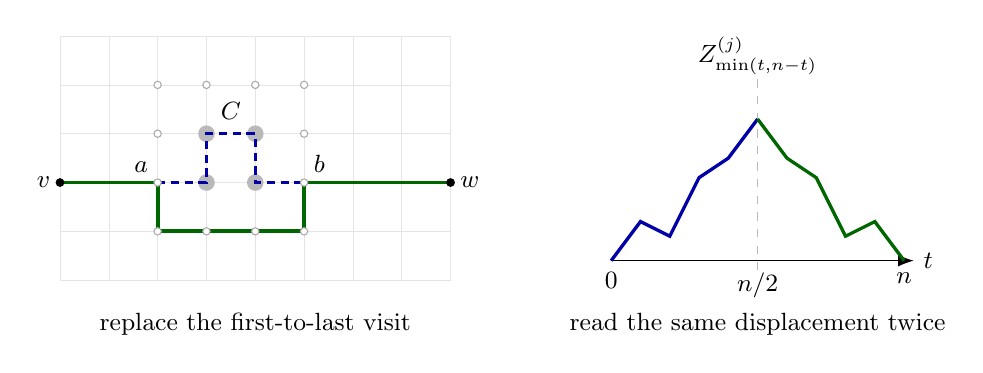
\begin{tikzpicture}[x=0.62cm,y=0.62cm,font=\small]
 \begin{scope}
  \draw[step=1,gray!20,very thin] (0,0) grid (8,5);
  \foreach \x/\y in {3/2,3/3,4/2,4/3}
   \fill[gray!55] (\x,\y) circle (0.17);
  \draw[blue!65!black,densely dashed,line width=1.1pt]
   (0,2)--(3,2)--(3,3)--(4,3)--(4,2)--(8,2);
  \draw[green!40!black,line width=1.4pt]
   (0,2)--(2,2)--(2,1)--(5,1)--(5,2)--(8,2);
  \foreach \x/\y in {2/1,3/1,4/1,5/1,5/2,5/3,5/4,4/4,3/4,2/4,2/3,2/2}
   \draw[gray!65,fill=white] (\x,\y) circle (0.075);
  \fill (0,2) circle (0.09) node[left] {$v$};
  \fill (8,2) circle (0.09) node[right] {$w$};
  \node[above left] at (2,2) {$a$};
  \node[above right] at (5,2) {$b$};
  \node[above] at (3.5,3.1) {$C$};
  \node[align=center] at (4,-0.9) {replace the first-to-last visit};
 \end{scope}
 \begin{scope}[xshift=7cm]
  \draw[-{Latex[length=2mm]}] (0,0.4)--(6.2,0.4) node[right] {$t$};
  \draw[gray!55,dashed] (3,0.2)--(3,4.2);
  \draw[blue!65!black,line width=1.2pt]
   (0,0.4)--(0.6,1.2)--(1.2,0.9)--(1.8,2.1)--(2.4,2.5)--(3,3.3);
  \draw[green!40!black,line width=1.2pt]
   (3,3.3)--(3.6,2.5)--(4.2,2.1)--(4.8,0.9)--(5.4,1.2)--(6,0.4);
  \node[below] at (0,0.35) {$0$};
  \node[below] at (3,0.35) {$n/2$};
  \node[below] at (6,0.35) {$n$};
  \node at (3,4.6) {$Z_{\min(t,n-t)}^{(j)}$};
  \node[align=center] at (3,-0.9) {read the same displacement twice};
 \end{scope}
\end{tikzpicture}
\caption{Two parts of the path construction, shown schematically.
Left: the original dashed route meets the finite bad component $C$;
the solid route joins its exterior predecessor $a$ to its exterior
successor $b$ through good nearest-neighbor vertices.  The drawing is a
planar schematic of a three-dimensional exterior shell, and does not
represent holes or later loop erasure.  Right: for even $n$, the random
transverse displacement used in the skeleton is reflected at $n/2$;
the common linear drift and integer rounding are omitted.  This return
to zero fixes the final endpoint without a bridge conditioning.}
\label{fig:lattice-detour}
\end{figure}

On $\mathcal E_{v,w}$, replace the visits of this lifted walk to bad
components as follows.  If it meets a lifted bad $*$-component $C$,
take its first and last visits to $C$.  The vertices immediately before
and after these visits belong to $\partial_*^{\rm ext}C$: the path
from the first endpoint to the first such vertex misses $C$, and the
path from the last such vertex to the other endpoint misses $C$;
both endpoints are outside $\operatorname{fill}(C)$.  By
Lemma~\ref{lattice:boundary}, join these two shell vertices by a simple
nearest-neighbor path in the shell, replacing the intervening part of
the walk.  The added vertices are all good.  Each replacement removes
at least one bad visit, and no replacement introduces a bad visit.
The process therefore terminates after finitely many steps.

Every component treated in this procedure was met by the original
nominal refinement: any remaining bad vertex still belongs to that
original walk.  Project the final walk to the torus and erase loops
in chronological order.  The result is a simple good nearest-neighbor
path from $v$ to $w$.  Every nonnominal vertex belongs to the shell of
a bad $*$-component met by $\Gamma$.  All choices in the refinement,
shell paths, and erasure can be made using fixed orderings.  Thus the
construction gives the measurable kernel in Proposition~\ref{prop:good-paths}.

We now bound the encounters introduced by this construction.  Use two
independent nominal samples $\Gamma,\Gamma'$ in the same environment,
and let $\pi,\pi'$ be their final simple paths.  Let $H$ range over
the range-$a_1$ bad components on the torus. Fix
$C_R=52(2R+1)^3$, which also exceeds $5(2R+1)$ in
Equation~\eqref{lattice:pair-occurrence}. On $\mathcal E_{v,w}$,
\begin{align}\label{lattice:detour-charge}
 J_R(\pi,\pi')
 &\le J_R(\Gamma,\Gamma')\notag\\
 &\quad+C_R\sum_H |H|
       \ind_{\{d_\infty(H,\Gamma)\le a_1,\,
                  d_\infty(H,\Gamma')\le a_1\}}.
\end{align}
For nominal walks, $J_R$ here counts vertex occurrences, which only
increases the bound.

To prove \eqref{lattice:detour-charge}, first count encounters where both
vertices are nominal.  These are bounded by the first term.  If a
nonnominal vertex belongs to the shell of $C$ and encounters a nominal
vertex of the other walk, then $C$ is within distance $R+1\le a_1$
of that other walk, and $C$ meets its own nominal walk.  If two
nonnominal vertices belong to shells of $C,C'$, then
$d_\infty(C,C')\le R+2\le a_1$, so both components belong to one
range-$a_1$ component $H$ meeting both nominal walks.  Charge each
such encounter to one of its nonnominal vertices and to this $H$.
There are at most $26|H|$ possible added vertices associated to the
$*$-components inside $H$, even if several lifted copies were used:
projection can only decrease this number.  Each such vertex encounters
at most $(2R+1)^3$ vertices of the other simple path.  Charging from
either path costs at most an additional factor two.  This proves the
claimed bound.

\subsection{Averaging the environment and applying both moments}

Fix both complete nominal paths.  Their independence from $\mathcal D$
leaves \eqref{lattice:bad-law} available for any prescribed collection of
bad vertices.  Expand the exponential of the second term in
\eqref{lattice:detour-charge} as a product over the actual range-$a_1$
components.  A term corresponding to distinct components has disjoint
vertex sets.  Drop maximality, sum over all disjoint connected candidate
sets, and apply \eqref{lattice:bad-law}.  Finally drop the disjointness
restriction and use $1+x\le e^x$.  The resulting bound is
\begin{align}\label{lattice:environment-expansion}
 &\E_{\mathcal D}\left[
 \ind_{\mathcal E_{v,w}}
 \exp\left(\kappa C_R\sum_H|H|
   \ind_{\{d_\infty(H,\Gamma),d_\infty(H,\Gamma')\le a_1\}}\right)
                       \right]\notag\\
 &\qquad\le
 \exp\left(\sum_F
       (p e^{\kappa C_R})^{|F|}
       \ind_{\{d_\infty(F,\Gamma),d_\infty(F,\Gamma')\le a_1\}}
                         \right),
\end{align}
where $F$ ranges over all nonempty range-$a_1$ connected torus sets.
The factor $e^{\kappa C_R|F|}-1$ from the expansion was bounded above
by $e^{\kappa C_R|F|}$.  Thus only joint bad-set probabilities were
used; there is no independence assumption on the environment.

We bound the exponent by the soft-distance statistic in
Equation~\eqref{lattice:imported-soft}. If a contributing set $F$ has size $m$,
choose an occurrence $z\in\Gamma$ within distance $a_1$ of a root of $F$.
There are at most $(2a_1+1)^3$ root choices for each $z$, and at most
$A_{a_1}^m$ connected sets at each root. A spanning-tree path in $F$ has
at most $m-1$ edges, each of length at most $a_1$ in the periodic maximum
metric. Since $F$ is also within $a_1$ of $\Gamma'$, the triangle inequality
gives
\[
 d_\infty(z,\Gamma')\le 2a_1+a_1(m-1)=a_1(m+1).
\]
This argument applies even to wrapping candidate sets; only the actual
components used for detours required the earlier lift and rejection test.
Absorb the root choices into a constant $A_R\ge1$. The exponent in
Equation~\eqref{lattice:environment-expansion} is at most
\begin{equation}\label{lattice:animal-series}
 \sum_{z\in\Gamma}\sum_{m\ge1}q^m
       \ind_{\{d_\infty(z,\Gamma')\le a_1(m+1)\}},
 \qquad q=A_Rp e^{\kappa C_R}.
\end{equation}
All constants here depend only on the fixed $R$. Counting the same set
more than once only increases this nonnegative upper bound.

Require $q\le e^{-2}$. If $d\le a_1(m+1)$, split $q^m$ into two equal
powers and use
\[
 q^m=q^{m/2}q^{m/2}\le q^{m/2}e^{-m}
                       \le e\,q^{m/2}e^{-d/a_1}.
\]
Summing the first factor over $m\ge1$ proves
\begin{equation}\label{lattice:soft-animal-sum}
 \sum_{m\ge1}q^m\ind_{\{d\le a_1(m+1)\}}
 \le\eta(p,\kappa)e^{-d/a_1},
 \qquad \eta(p,\kappa)=\frac{e\sqrt q}{1-\sqrt q}.
\end{equation}
In particular $\eta(p,\kappa)\to0$ as $p\to0$ at fixed $\kappa$.
Set $B=a_1$. Equations~\eqref{lattice:detour-charge},
\eqref{lattice:pair-occurrence}, and
\eqref{lattice:environment-expansion}--\eqref{lattice:soft-animal-sum} give
\begin{equation}\label{lattice:moment-reduction}
 \E_{\mathcal D}\left[
  \ind_{\mathcal E_{v,w}}e^{\kappa J_R(\pi,\pi')}
       \mid\Gamma,\Gamma'\right]
 \le\exp\left(\kappa C_RJ_{\rm occ}^{(R)}+
                      \eta(p,\kappa)S_B(\Gamma,\Gamma')\right).
\end{equation}
On the left, the adapted paths are used only on $\mathcal E_{v,w}$.
The environment was averaged once, with both entire skeletons fixed.

First choose $\kappa>0$ with $2\kappa C_R\le\alpha_R$, where
$\alpha_R=c_{\rm hit}/(1+R)^2$. Next choose $p_0>0$ so small that
$q\le e^{-2}$ and $2\eta(p,\kappa)\le\xi(B)$ for $p\le p_0$, as well
as the earlier endpoint rejection requirements. The constants $K_0$ can
then be enlarged to cover those rejection estimates. Cauchy--Schwarz and
both moments in Lemma~\ref{lem:skeleton} imply
\begin{align*}
 \E\exp\left(\kappa C_RJ_{\rm occ}^{(R)}+\eta S_B\right)
 &\le
 \left(\E e^{2\kappa C_RJ_{\rm occ}^{(R)}}\right)^{1/2}
 \left(\E e^{2\eta S_B}\right)^{1/2}\\
 &\le\sqrt{C_{\rm hit}C(B)}=:C_{\rm path}<\infty.
\end{align*}
Together with Equation~\eqref{lattice:moment-reduction}, this proves the
annealed bound~\eqref{eq:lattice-encounter}. Both path draws use one common
datum and independent skeleton seeds. The event retains its original
mass; there is no renormalization by conditioning on acceptance and no
assertion of a bound for each fixed environment.

Finally, for $K\ge80$ the interval
$[\lceil K/10\rceil,\lfloor K/8\rfloor]$ contains at least
$K/40-1\ge K/80$ integers. For each such $n$, there are
$(2n+1)^2\ge K^2/25$ transverse choices. They are distinct modulo $K$,
since $2n<K$. Multiplying by the $K^3$ choices of starting vertex gives
at least $K^6/2000=\upsilon K^6$ admissible ordered pairs. This completes
Proposition~\ref{prop:good-paths}.

\section{A common measure and positive occupation}
\label{sec:comparison}

We now turn the supply of movable labels into a lower bound on the
constant-orbital fraction $B_{\rm occ}$. Recall from
Proposition~\ref{prop:purification} that the midpoint configuration $X$ and
the retained configuration $W'$ have density $\Phi(X,W')^2$, where $\Phi$
is the nonnegative kernel of the square root of the canonical state.
The input is the conditional path law of Section~\ref{sec:groups} and the
good lattice routes of Proposition~\ref{prop:good-paths}. Along one route
we construct two copies of the selected trajectories. Their midpoint
assignments leave the same observed bath after different tags are removed.
We then bound the second moment of the resulting change of measure by
encounters between two routes.

This is the comparison mechanism of \citet[Section~8]{HS}; its conditional
normalizer argument is reproduced below. The thermal modification is to
retain $W'$ in every observation and in the exposed data. It is never
resampled. All constants obtained here are uniform in $D,K$ and
$0<T\le D^{-1}$ once the earlier fixed parameters have been chosen.

\subsection{Affinity and a common finite measure}

For finite nonnegative measures $P,Q$ on the same measurable space, define
their affinity by
\[
 \Aff(P,Q)=\int\sqrt{pq}\dd\xi,
 \qquad p=\frac{\dd P}{\dd\xi},\quad q=\frac{\dd Q}{\dd\xi},
 \quad \xi=P+Q.
\]
Using another dominating measure gives the same value. We will use three
elementary properties. If $P\ge P'$ and $Q\ge Q'$, then
$\Aff(P,Q)\ge\Aff(P',Q')$. For finite lists of measure pairs,
\begin{equation}\label{cmp:affinity-superadditive}
 \Aff\left(\sum_jP_j,\sum_jQ_j\right)
 \ge\sum_j\Aff(P_j,Q_j).
\end{equation}
Indeed, pointwise Cauchy--Schwarz gives
$\sum_j\sqrt{p_jq_j}\le\sqrt{(\sum_jp_j)(\sum_jq_j)}$.
Finally, applying the same probability kernel to both measures cannot decrease
affinity. To see this, form the joint measures with that kernel and then
condition a common dominating measure on the output. Conditional
Cauchy--Schwarz gives
$\E(\sqrt{pq}\mid\text{output})\le
\sqrt{\E(p\mid\text{output})\E(q\mid\text{output})}$.
Integration proves the assertion. Projection is a special case.

\begin{lemma}[A common finite measure]\label{lem:affinity}
Let $P,Q$ be finite nonnegative measures and let $\nu$ be a finite measure
of mass $m>0$, absolutely continuous with respect to both. If
\[
 \int\left(\frac{\dd\nu}{\dd P}\right)^2\dd P\le C_P,
 \qquad
 \int\left(\frac{\dd\nu}{\dd Q}\right)^2\dd Q\le C_Q,
\]
then $\Aff(P,Q)\ge m^2/\sqrt{C_PC_Q}$.
\end{lemma}
\begin{proof}
With densities $p,q,s$ relative to a common dominating measure, H\"older's
inequality with exponents $4,4,2$ gives
\[
 m=\int
 \left(\frac{s^2}{p}\right)^{1/4}
 \left(\frac{s^2}{q}\right)^{1/4}(pq)^{1/4}
 \le C_P^{1/4}C_Q^{1/4}\Aff(P,Q)^{1/2}.
\]
The ratios can be set to zero where their denominators vanish, since $s$ is
zero there. Squaring and rearranging proves the claim.
\end{proof}

\subsection{Cell measures and disjoint groups of tags}

Recall $V=K^3$, $D=N/V$, and the unit cells $B_v$, each of volume one.
Write $X'=(x_2,\ldots,x_N)$ for the ordered bath. For ordered cells $v,w$,
define finite measures on
$(x,y,X',W')\in B_v\times B_w\times\Lambda_K^{N-1}\times\Lambda_K^N$ by
\begin{equation}\label{cmp:cell-measures}
\begin{aligned}
 \dd P_{vw}=V\Phi(x,X',W')^2\dd x\dd y\dd X'\dd W',
 \\
 \dd Q_{vw}=V\Phi(y,X',W')^2\dd x\dd y\dd X'\dd W'.
\end{aligned}
\end{equation}
Nonnegativity of $\Phi$ and the occupation formula in
Proposition~\ref{prop:purification} give the exact identity
\begin{equation}\label{cmp:cell-affinity}
 B_{\rm occ}=\frac1{V^2}\sum_{v,w}\Aff(P_{vw},Q_{vw}).
\end{equation}

Fix a group index
$1\le g\le G_D:=\lfloor\ell D/(4M)\rfloor$ from
Section~\ref{sec:groups}. Its exposed data are $\cB$, its unexposed label
set is $\cI$, and its conditional path law is $\lambda_{\cI}$ from
Lemma~\ref{lem:conditional-law}. Define measures
$\widehat P_g,\widehat Q_g$ on $(\cB,x,y,X')$; the data $\cB$ already
include $W'$.
For $\widehat P_g$, sample the data and the conditional unexposed paths, and
\emph{sum} the following contributions over all $i\in\cI$:
take $x=\omega_i(t)$, restrict to $x\in B_v$, order the remaining $N-1$
midpoints by a fresh uniform permutation to form $X'$, and sample $y$
uniformly in $B_w$. For $\widehat Q_g$, take the tagged midpoint as
$y\in B_w$ and sample the extra point $x$ uniformly in $B_v$.
The use of a sum, rather than a uniformly chosen tag, fixes their
normalization.

\begin{lemma}[Tag normalization]\label{lem:tag-normalization}
For each ordered pair of cells,
\begin{equation}\label{cmp:group-affinity}
 \Aff(P_{vw},Q_{vw})
 \ge\frac1D\sum_{g=1}^{G_D}\Aff(\widehat P_g,\widehat Q_g).
\end{equation}
\end{lemma}
\begin{proof}
Put all groups on the original slab sample, with all allocation
randomizations and a fresh uniform permutation of the full label set.
After deleting a tag, the restricted permutation uniformly orders its bath.
Each group's conditional construction is a disintegration of this common
sample with respect to its own exposed data. Thus the differing data spaces
are projected away before the following comparison; no conditional symmetry
of the unexposed-path law is asserted.
For every sampled path configuration, group label sets are disjoint. Their
sum of tag contributions is bounded by the sum over all $N$ trajectory
labels. The unrestricted midpoint vector together with $W'$ has density
$\Phi(X,W')^2$, symmetric in $X$ for each $W'$.
For each fixed tag label, uniform ordering of the bath therefore gives the
same density $\Phi(x,X',W')^2$. Summing all tags gives $N$ times that density.
Since the extra target cell has volume one and $V/N=1/D$, projecting to
$(x,y,X',W')$ yields
\[
 \frac1D\sum_g\operatorname{proj}\widehat P_g\le P_{vw},
 \qquad
 \frac1D\sum_g\operatorname{proj}\widehat Q_g\le Q_{vw}.
\]
Use monotonicity, \eqref{cmp:affinity-superadditive}, and the increase of
affinity under projection. Its homogeneity supplies the factor $1/D$.
\end{proof}

The remaining task is to find, for each retained group and each of many
ordered cell pairs, a common measure of mass at least $1/2$ whose squared
likelihood integrals against $\widehat P_g$ and $\widehat Q_g$ are bounded
by one constant $C_2$. Lemma~\ref{lem:affinity} would then give affinity at
least $1/(4C_2)$ per group. The factor $1/D$ in
Equation~\eqref{cmp:group-affinity} can be paid because the number of
disjoint groups is proportional to $D$.

\subsection{Two midpoint assignments with the same observed bath}

Take $R=30$ in Proposition~\ref{prop:good-paths}, and fix an admissible
ordered cell pair $v,w$: its lift displacement $(n,d_2,d_3)$ satisfies
$\lceil K/10\rceil\le n\le\lfloor K/8\rfloor$ and $|d_i|\le n$.
Choose the good-site
parameters of Proposition~\ref{prop:group-supply} to meet the bad-set hypothesis
of Proposition~\ref{prop:good-paths}. Let $\mathcal E_{vw}$ be the data-measurable
event supplied by Proposition~\ref{prop:good-paths}, of probability at least $1/2$. On this event draw a simple nearest-neighbor
path
\[
 z_0=v,z_1,\ldots,z_d=w
\]
through good sites. For each $k<d$, independently choose a uniform accessible
label $i_k$ anchored at $z_k$. The choices inspect only $\cB$ and the lattice
path. In particular, they do not inspect any latent trajectory. The selected
labels are distinct because their anchors are distinct.

We construct two path configurations that share their observed $(x,y,X',W')$.
Keep the exposed data fixed. First sample all unselected unexposed
trajectories from their exact marginal under $\lambda_{\cI}$, and use
them in both copies. For every vertex $z_k$, prepare a factor as follows.
The first copy needs label $i_k$ through this cell if $k<d$, and the second
copy needs label $i_{k-1}$ through it if $k>0$. Intersect the corresponding
good-target sets $T_{i_k}(z_k)$ and $T_{i_{k-1}}(z_k)$ from
Section~\ref{sec:groups}, using only the one required set at an endpoint.
The intersection, denoted by $A_k$, has volume at least $0.98$.
Sample $U_k$ uniformly in $A_k$, and then independently sample the one or
two required bridge trials through $U_k$, each conditioned on its individual
success against the frozen paths. All $d+1$ vertex factors are independent
before the additional conditioning below. Figure~\ref{cmp:shift-figure}
shows the two midpoint assignments.

Use $U_d$ as the extra point in the first copy and $U_0$ as the extra point
in the second copy. Impose all remaining hard-avoidance checks in both
copies: selected paths must avoid the unselected unexposed paths and one another
within their respective copies. Condition the product of vertex factors on
these checks, separately for each fixed collection of unselected paths.
The sampled unselected-path marginal therefore remains its original marginal
under $\lambda_{\cI}$.
More explicitly, let $\lambda_{\rm out}$ be that marginal, let $F_k$ be
the probability law of the $k$th vertex factor, and let $J$ be the
indicator of the remaining checks in both copies. The joint law just
defined is
\begin{equation}\label{cmp:fixed-outside-law}
 \lambda_{\rm out}(\dd\omega_{\rm out})\,
 \frac{J(\omega_{\rm out},\xi_0,\ldots,\xi_d)
             \prod_{k=0}^d F_k(\dd\xi_k)}
      {\displaystyle\int J(\omega_{\rm out},\xi_0,\ldots,\xi_d)
             \prod_{k=0}^d F_k(\dd\xi_k)}.
\end{equation}
The denominator is a function of the fixed outside paths. Integrating the
second factor gives one for each such configuration. A single normalization
after integrating the outside paths would change their marginal and would
not yield the comparison used below. Each $F_k$ depends only on the data,
route and selected labels, so it is fixed before those outside paths are
sampled.

We verify that this conditional construction is defined. A vertex factor
carries at most two paths, each with a marginal of the form $\Pi_i^{A_k}$
in Proposition~\ref{prop:group-comparison}. Its paths are confined within distance
ten of their anchors, and there are at most $M$ unexposed labels per anchor.
Consequently each factor has at most $C_{\rm col}M$ possible opponents in the two
copies, for a fixed geometric constant $C_{\rm col}$. All opponents have distinct labels within the copy in which a check
is imposed. The deterministic-opponent estimate, summed over those checks,
gives
\begin{equation}\label{cmp:compatibility}
 \chi_D=C_{\rm col}M e_D\longrightarrow0
 \qquad(D\longrightarrow\infty,\ M\text{ fixed}).
\end{equation}
For any fixed regular and confined values of the other paths with their
recorded endpoints, the factor passes every incident check with probability
at least $1-\chi_D$.
This statement averages its common midpoint over $A_k$; it makes no claim at
a prescribed midpoint. It uses the two path marginals and a union bound,
so no independence of the paths within the factor is required. Inserting
the $d+1$ factors successively now bounds the two-copy conditioning
probability below by $(1-\chi_D)^{d+1}>0$ for sufficiently large $D$.

Tag $i_0$ in the first copy and $i_{d-1}$ in the second. In each copy the
tag and the extra point then give $x=U_0$, $y=U_d$. The selected bath
midpoints in both copies are exactly $U_1,\ldots,U_{d-1}$; the unselected
midpoints also agree. Choose a common uniform ordering of the shared midpoint instances; their
physical labels in the two copies may differ. In each copy separately,
this has the uniform ordering law determined by its paths and its tag.
This defines a single finite measure $\widehat\nu$ on $(\cB,x,y,X')$ after
averaging the data, routes and labels, with zero mass off $\mathcal E_{vw}$.
Each conditional sampling law on this event is a probability measure, so
\begin{equation}\label{cmp:common-mass}
 \widehat\nu(\text{all})=\PP(\mathcal E_{vw})\ge\frac12.
\end{equation}
These are measurable probability kernels: the route and label choices are
finite, the target sets are measurable functions of the data, and all
path restrictions are Borel subsets of the continuous-path spaces. The
positive normalizers just proved permit the displayed conditioning.

\begin{figure}[t]
\centering
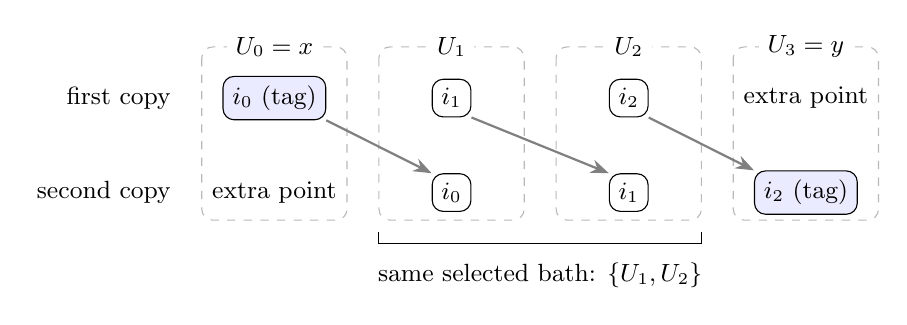
\begin{tikzpicture}[x=2.25cm,y=1cm,>=Stealth,
  every node/.style={font=\small}]
 \foreach \x/\txt in {0/{U_0=x},1/{U_1},2/{U_2},3/{U_3=y}} {
   \draw[gray!55,dashed,rounded corners]
          (\x-.41,.65) rectangle (\x+.41,-1.55);
   \node[fill=white,inner sep=3pt] at (\x,.65) {$\txt$};
 }
 \node[anchor=east] at (-.53,0) {first copy};
 \node[anchor=east] at (-.53,-1.2) {second copy};
 \node[draw,rounded corners,fill=blue!8] (a0) at (0,0) {$i_0$ (tag)};
 \node[draw,rounded corners,fill=white] (a1) at (1,0) {$i_1$};
 \node[draw,rounded corners,fill=white] (a2) at (2,0) {$i_2$};
 \node at (3,0) {extra point};
 \node at (0,-1.2) {extra point};
 \node[draw,rounded corners,fill=white] (b1) at (1,-1.2) {$i_0$};
 \node[draw,rounded corners,fill=white] (b2) at (2,-1.2) {$i_1$};
 \node[draw,rounded corners,fill=blue!8] (b3) at (3,-1.2) {$i_2$ (tag)};
 \draw[->,gray,thick] (a0.south east) -- (b1.north west);
 \draw[->,gray,thick] (a1.south east) -- (b2.north west);
 \draw[->,gray,thick] (a2.south east) -- (b3.north west);
 \draw (.59,-1.7) -- (.59,-1.85) -- (2.41,-1.85) -- (2.41,-1.7);
 \node at (1.5,-2.25) {same selected bath: $\{U_1,U_2\}$};
\end{tikzpicture}
\caption{The midpoint assignment for a route of three edges. A dashed
column is one vertex factor with one common midpoint. Arrows identify the
same particle label in the two copies; they are not trajectories in time.
Removing the highlighted tags leaves the same two selected bath midpoints.
All unselected bath paths and the configuration $W'$ are shared. For a
route of arbitrary length the interior columns continue in the same way.}
\label{cmp:shift-figure}
\end{figure}

\subsection{Cancellation of conditional normalizers}

The midpoint construction has two path copies in each internal vertex
factor. To estimate its likelihood, designate one copy as primary and regard
the other as auxiliary. At an internal vertex $z_k$, $1\le k<d$, the
primary path has label $i_k$ in the first-copy view, whereas the auxiliary
path has label
$i_{k-1}$. Thus deleting a factor is not the same operation as deleting all
instances of one particle label. The following lemma keeps this distinction
explicit and isolates the normalizers that cancel when two routes are far
apart. Its coordinates and factors are abstract; we identify them with the
midpoint construction immediately after the proof.
The two changes arise because the square of a route-averaged likelihood
expands into a product for two independent route choices at the same
exposed datum.

The next lemma, from \citet[Lemma~8.3]{HS}, concerns finitely many
coordinates in standard Borel spaces,
each with a probability reference $P_i$. All auxiliary spaces below are
standard Borel as well. A \emph{check} will mean an indicator imposing a constraint
on one or two coordinates. The joint reference law $\lambda$ is the product
$\bigotimes_iP_i$ conditioned on a finite collection of checks. An additional
independent coordinate is allowed; it simply has no checks.

A change indexed by a set $S$ leaves the marginal outside $S$ unchanged.
Inside $S$, it starts from independent factors $\Pi_{S,i}$, $i\in S$.
Each factor includes a \emph{primary coordinate} in the space of $P_i$ and
possibly auxiliary coordinates. Its primary marginal is $g_{S,i}P_i$, with
\begin{equation}\label{cmp:factor-density}
 0\le g_{S,i}\le G,
 \qquad \int g_{S,i}\dd P_i=1.
\end{equation}
The factors are fixed before the outside coordinates are sampled. The product
is conditioned on specified checks, including every reference check involving
the primary coordinates in $S$. Checks involving only fixed outside
coordinates are already satisfied almost surely under the unchanged outside
marginal; otherwise the conditional proposal would not be defined there.
Omit these redundant checks. Every remaining proposal check therefore
involves a coordinate carried by a changed factor. Auxiliary coordinates
are then forgotten.
The resulting primary likelihood relative to $\lambda$ is denoted by $L_S$.

For each primary and auxiliary coordinate, fix a measurable allowed set
on which all its relevant reference and proposal marginals are
concentrated. These sets, like the proposal factors, are fixed before
sampling outside coordinates. A configuration is \emph{individually
permitted} when each coordinate lies in its allowed set; this imposes no
pairwise checks. The compatibility hypothesis below is uniform on these
sets, including configurations that fail some pairwise checks.

We make explicit the deletion convention for this construction. When some
factors are removed, remove their coordinates and all checks incident to them.
Do not replace a removed auxiliary coordinate by an original reference
coordinate. Coordinates fixed outside the sets under discussion remain as
obstacles in all the checks in which they occur. Coordinates here are path
instances in a specified copy. If an auxiliary with label $j$ belongs to a
retained factor, it remains integrated in that factor even when a different
factor carrying the primary label $j$ is deleted. It is never replaced by
the original path with label $j$.

\begin{lemma}[Cancellation away from an overlap]\label{lem:cancellation}
Consider two changes $S,T$ of the preceding kind, with $G\ge1$, and put
$U=S\cup T$. Suppose that the following conditions hold.
\begin{enumerate}
 \item[(i)] There is $\chi\in[0,1)$ with two insertion bounds.
 In the reference system, inserting any coordinate $i\in U$ from $P_i$
 satisfies all reference checks incident to $i$ with probability at least
 $1-\chi$. In the proposal system of either change, inserting a whole
 factor from $\Pi_{S,i}$ or $\Pi_{T,i}$ satisfies all checks of that
 proposal incident to its carried coordinates with probability at least
 $1-\chi$. Each bound is uniform in every fixed choice of the other
 individually permitted coordinates of the respective system, and remains
 valid after deleting checks or coordinates as specified above.
 \item[(ii)] There are decompositions $S=C_S\sqcup F_S$ and
 $T=C_T\sqcup F_T$, with $F_S\cap T=F_T\cap S=\varnothing$.
 No coordinate carried by an $F_S$ factor has a check with any coordinate
 carried by a $T$ factor, or with the original primary coordinates indexed
 by $T$; the corresponding assertion holds with $S,T$ interchanged.
 The reference coordinates in $F_S,F_T$ also have no mutual checks.
\end{enumerate}
Then
\begin{equation}\label{cmp:cancellation-bound}
 \int L_SL_T\dd\lambda
 \le G^{|S\cap T|}(1-\chi)^{-2(|C_S|+|C_T|)}.
\end{equation}
It is enough that the assumptions hold for almost every fixed admissible
configuration outside $U$.
\end{lemma}

\begin{proof}
Put $a_\chi=1-\chi$ and $c=|C_S|+|C_T|$. Fix the primary coordinates
outside $U$. All normalizers below are conditional on these fixed values;
we first work on a configuration for which this conditional law is defined.

For any selected set, its reference normalizer is the integral of its
reference-check indicator against its product references. In particular,
write $Z_U$ for this integral over $U$. When the coordinates outside $S$
are fixed, write $Z_S$ for the corresponding integral over $S$. Thus $Z_S$
can depend on coordinates in $T\setminus S$. Write $Y_S$ for the integral
of the proposal-check indicator $J_S$ against $\bigotimes_{i\in S}\Pi_{S,i}$,
with the same outside values fixed.

Disintegrate each factor in the form
\[
 \Pi_{S,i}(\dd x_i\,\dd\zeta_i)
   =P_i(\dd x_i)K_{S,i}(x_i,\dd\zeta_i),
 \qquad K_{S,i}(x_i,\text{all})=g_{S,i}(x_i).
\]
Here $\zeta_i$ denotes all its auxiliary coordinates. Define
\[
 H_S(x_S;x_{S^c})
  =\int J_S\prod_{i\in S}K_{S,i}(x_i,\dd\zeta_i).
\]
On the reference-admissible configurations, the exact likelihood is
\begin{equation}\label{cmp:exact-likelihood}
 L_S=\frac{Z_S}{Y_S}H_S.
\end{equation}
Indeed, the conditional reference density is its check indicator divided by
$Z_S$, whereas the new primary density is $H_S/Y_S$, both relative to
$\bigotimes_{i\in S}P_i$. The outside marginal is identical. The inclusion
of primary reference checks ensures that the new density is zero on
reference-forbidden configurations.

Now retain only the factors indexed by $F_S$, together with coordinates fixed
outside $U$, using the stated deletion convention. Denote their reference
normalizer, proposal normalizer and primary proposal density by
$Z_{F_S},Y_{F_S},H_{F_S}$. Define the three corresponding $F_T$ quantities
using the factors from the $T$ change. These quantities depend only on the
outside of $U$ and, for $H_{F_S},H_{F_T}$, on their own primary coordinates.
They do not depend on the omitted near coordinates.

Successive insertion using assumption~\textup{(i)}, and noninteraction in
assumption~\textup{(ii)}, give
\begin{align}
 Z_U&\ge a_\chi^c Z_{F_S}Z_{F_T},
       \label{cmp:union-normalizer}\\
 Z_S&\le Z_{F_S},\qquad
 Y_S\ge a_\chi^{|C_S|}Y_{F_S},
       \label{cmp:single-normalizers}\\
 Z_T&\le Z_{F_T},\qquad
 Y_T\ge a_\chi^{|C_T|}Y_{F_T}.
       \label{cmp:other-normalizers}
\end{align}
For the first inequality, the reference integral over the two far sets
factorizes. The remaining distinct coordinates form
$U\setminus(F_S\cup F_T)$, a subset of $C_S\cup C_T$ with cardinality
at most $c$. Insert them one at a time with the uniform compatibility
bound. For the upper
bound on $Z_S$, delete the checks involving $C_S$ and integrate those reference
coordinates freely. Coordinates in $T\setminus S$ have no checks with the
far set. For its proposal lower bound, start with the reduced $F_S$ integral
and add the $C_S$ factors. The fixed original coordinates in
$T\setminus S$ still do not meet the far factors. An auxiliary instance
carried by a retained factor remains integrated there, even if a newly
inserted factor carries its primary label; only the checks of the $S$
proposal are restored. Each addition retains at
least the factor $a_\chi$. Applying these two arguments to the $T$ change proves the
last line. These statements are pointwise in the opposing coordinates;
they do not assert that $Z_S$ or $Y_S$ is constant in them.

The insertion bounds also prove positivity of the divisors. In particular,
integrating coordinates one at a time gives a positive product lower bound
for every reduced normalizer. The full reference conditional is defined on
the outside configurations under consideration.

Deleting proposal checks involving a near factor gives
\[
 H_S\le H_{F_S}\prod_{i\in C_S}g_{S,i},
 \qquad
 H_T\le H_{F_T}\prod_{i\in C_T}g_{T,i}.
\]
After dropping the reference admissibility indicator in an upper bound,
the two far primary integrals equal $Y_{F_S}$ and $Y_{F_T}$. The remaining
coordinates carry only the displayed marginal densities. A coordinate
occurring once integrates to one. A coordinate occurring in both lists
costs at most $G$, by \eqref{cmp:factor-density}. Therefore
\begin{equation}\label{cmp:kernel-product}
 \int H_SH_T\ind_{\mathrm{admissible}}
              \prod_{i\in U}P_i(\dd x_i)
 \le Y_{F_S}Y_{F_T}G^{|S\cap T|}.
\end{equation}
The conditional reference law on $U$ has normalizer $Z_U$. Combine
\eqref{cmp:exact-likelihood}--\eqref{cmp:kernel-product}. The two pointwise
ratio bounds contribute
$a_\chi^{-c}Z_{F_S}Z_{F_T}/(Y_{F_S}Y_{F_T})$; division by $Z_U$
contributes at most $a_\chi^{-c}/(Z_{F_S}Z_{F_T})$. All four far
normalizers cancel, leaving $G^{|S\cap T|}a_\chi^{-2c}$.
Finally integrate the outside coordinates. This proves
\eqref{cmp:cancellation-bound}.
\end{proof}

\subsection{The likelihood cost is confined to encounters}

Fix the data, the route and the selected labels. Regard either copy as the
primary one. The reference for that copy is
$\lambda_{\cI}\otimes P_*$, where $P_*$ is the uniform law of the extra
point in its endpoint cell. Let
\[
 S=\{i_0,\ldots,i_{d-1}\}\cup\{*\}.
\]
In Lemma~\ref{lem:cancellation}, a primary coordinate is the chosen copy's
path or endpoint extra point. Its auxiliary coordinates are the other
copy's path or extra point through the same midpoint. The checks are the
collision exclusions within each copy; there is no collision check between
paths in different copies.
Index a vertex factor by its primary label, using $*$ for the extra point;
its center is its midpoint cell $z_k$. The two paths in one factor may have
different labels, and each copy contributes at most one path. The allowed
set for each path consists of the regular, confined, frozen-avoiding paths
with its own recorded endpoints. Each extra point lies in its target cell.
These are individual restrictions; the remaining collision checks still
couple different factors.

By Proposition~\ref{prop:group-comparison}, the primary marginal of each path
factor has density at most $G$ relative to $P_i$, and integrates to one.
For the extra point the density is $\ind_{A_k}/|A_k|$ relative to $P_*$,
which is at most $1/0.98$. Enlarge the fixed $G$ to be at least two, covering
this factor as well. These marginal densities and their auxiliary kernels
depend on the exposed data and the route and label choices; they do not
depend on the unselected unexposed paths.

The union bound proving Equation~\eqref{cmp:compatibility} verifies
hypothesis~\textup{(i)} for each proposal factor. The same argument with
$P_i$ in place of $\Pi_i^{A_k}$ verifies it for insertion of a selected
reference path, by Proposition~\ref{prop:group-comparison}. The reference extra
point has no checks. These estimates are uniform over all individually
permitted opponent paths, whether or not their labels are accessible, and
deleting checks can only improve them. Thus the bound remains available
for every reduced normalizer in Lemma~\ref{lem:cancellation}.

Take two independent route and label choices at the same data and endpoint
pair, and denote their selected index sets by $S,T$. For the chosen primary
side, declare a factor of $S$ near if its center is at lattice supremum
distance at most $R$ from some center of $T$, and declare every other factor
far. Define $C_S,F_S,C_T,F_T$ accordingly. A shared real label has centers
at distance at most two in the two assignments, so it is near; the shared
extra index has the same endpoint center. Consequently the far index sets
are disjoint from the opposing lists.

All paths carried by a factor lie within distance eleven of its center.
The original path of an opposing real label also lies within distance eleven
of that opposing factor's center. Since $R=30$, far factors cannot interact
with any coordinate carried by the opposite list or with those original
paths. This includes the auxiliary-copy paths. Far sets therefore meet the
separation assumptions of Lemma~\ref{lem:cancellation}.

For clarity, a reduced far proposal retains exactly the paths carried by
its far vertex factors and the fixed paths outside $S\cup T$. It deletes
the omitted near factors in both copies. It does not put their original
trajectories back as unselected obstacles. With this convention all the
normalizers in \eqref{cmp:union-normalizer}--\eqref{cmp:kernel-product}
are the ones arising from the present construction.

Write $L_S,L_T$ for the two primary likelihoods. If
\[
 J_R=\#\{(j,k):d_\infty(z_j,z'_k)\le R\},
\]
then $|C_S|+|C_T|\le2J_R$. Lemma~\ref{lem:cancellation} gives, at the
fixed data,
\begin{equation}\label{cmp:two-choice-bound}
 \int L_SL_T\dd(\lambda_{\cI}\otimes P_*)
 \le G^{|S\cap T|}(1-\chi_D)^{-4J_R}.
\end{equation}
In particular, no factor is paid for a long portion of one route that stays
away from the other.

\subsection{Averaging labels and forgetting the paths}

Condition on the data and the two lattice paths before choosing their labels.
Each common departure cell has at least $M/2$ accessible labels. The two
uniform choices at that cell match with probability at most $2/M$, and the
match events are independent between distinct common cells. Real labels
anchored at different cells cannot agree. The shared extra point contributes
one factor $G$, so
\begin{equation}\label{cmp:label-average}
 \E_{\mathrm{labels}}G^{|S\cap T|}
 \le G\exp\left(\frac{2(G-1)}M J_R\right).
\end{equation}
Choose the fixed integer $M$ sufficiently large for the good-site supply
and for
\begin{equation}\label{cmp:M-choice}
 \frac{2(G-1)}M\le\frac\kappa2.
\end{equation}
Then increase $D_*$ so that, for every $D\ge D_*$ in the allowed $\alpha$
window, all earlier estimates hold and
\begin{equation}\label{cmp:D-choice}
 -4\log(1-\chi_D)\le\frac\kappa2,
 \qquad
 \frac{G_D}{D}\ge\frac\ell{8M}.
\end{equation}
The first requirement is possible by \eqref{cmp:compatibility}; the second
follows once $\ell D/(4M)\ge2$. These choices do not change $G$, $\kappa$,
or $C_{\mathrm{path}}$.

The following use of an averaged likelihood and a two-route second moment
also occurs in the point-reassignment argument of
Peres and Sly~\cite[Proposition~2.1]{PeresSly2014}. Here
Lemma~\ref{lem:cancellation} supplies the additional conditional-normalizer
estimate required by the hard-core path law.

Let $\overline L$ be the likelihood averaged over the conditional route and
label choices, with value zero off $\mathcal E_{vw}$. Tonelli's theorem
expresses its square integral using two independent such choices. Combining
\eqref{cmp:two-choice-bound}--\eqref{cmp:D-choice} and the annealed encounter
bound in Proposition~\ref{prop:good-paths} gives
\begin{equation}\label{cmp:latent-second-moment}
 \E_{\cB}\int\overline L^{2}
           \dd(\lambda_{\cI}\otimes P_*)
 \le G\E\bigl[\ind_{\mathcal E_{vw}}e^{\kappa J_R}\bigr]
 \le C_2,
 \qquad C_2:=G C_{\mathrm{path}}.
\end{equation}
Here the two route randomizations share the same data; the expectation over
the data is taken only once. The event is not conditioned to have probability
one. Its indicator is part of both likelihoods, and its square is itself.
The calculation applies separately with either copy primary, with the same
constant $C_2$.

We next check carefully that tagging and observing the bath do not increase
this bound. At fixed data, split $\overline L=\sum_{i\in\cI}f_i$, where
$f_i$ contains exactly the choices designating $i$ as the primary tag.
The functions are nonnegative. In the first copy $f_i$ is supported where
$\omega_i(t)\in B_v$; in the second it is supported where
$\omega_i(t)\in B_w$. Since
\[
 \sum_i f_i^2\le\left(\sum_i f_i\right)^2,
\]
the measure that retains the tag index has squared likelihood integral at
most $C_2$ relative to the \emph{sum} of the tag-restricted reference
measures on the disjoint copies indexed by $i$. Now apply the observation kernel that orders the bath and retains
$\cB,x,y,X'$, and forget the tag and all the paths. If a finite measure has
density $f$ relative to a reference $P$, the density after applying a common
kernel is the conditional average of $f$ in the corresponding joint
reference measure. Conditional Cauchy--Schwarz bounds its squared integral
by $\int f^2\dd P$. This remains valid for finite reference measures,
by normalization when their mass is nonzero.

For either primary copy, the resulting measure is the common observed
$\widehat\nu$ already constructed. Its corresponding reference is precisely
$\widehat P_g$ or $\widehat Q_g$. We have proved
\begin{equation}\label{cmp:observed-second-moments}
 \int\left(\frac{\dd\widehat\nu}{\dd\widehat P_g}\right)^2
                \dd\widehat P_g\le C_2,
 \qquad
 \int\left(\frac{\dd\widehat\nu}{\dd\widehat Q_g}\right)^2
                \dd\widehat Q_g\le C_2.
\end{equation}
Together with \eqref{cmp:common-mass}, Lemma~\ref{lem:affinity} now gives
\begin{equation}\label{cmp:one-group-gain}
 \Aff(\widehat P_g,\widehat Q_g)\ge\frac1{4C_2}.
\end{equation}
This lower bound is uniform in the group index and in every admissible
ordered pair of cells.

\begin{proof}[Proof of Theorem~\ref{thm:scaled}]
With the fixed choices above, set
\begin{equation}\label{cmp:c-star}
 c_*:=\frac{\upsilon\ell}{32M G C_{\mathrm{path}}}>0,
 \qquad \upsilon=\frac1{2000}.
\end{equation}
For large $K$, at least $\upsilon V^2$ ordered cell pairs meet the displacement
condition of Proposition~\ref{prop:good-paths}. For each such pair,
Lemma~\ref{lem:tag-normalization}, \eqref{cmp:D-choice} and
\eqref{cmp:one-group-gain} give
\[
 \Aff(P_{vw},Q_{vw})
 \ge\frac{G_D}{4D C_2}
 \ge\frac\ell{32M C_2}.
\]
Sum these nonnegative contributions in \eqref{cmp:cell-affinity} to obtain
$B_{\rm occ}\ge\upsilon\ell/(32M C_2)$, which is \eqref{cmp:c-star}.
Every estimate used above is uniform over the stated temperature interval.
The volume threshold is locally uniform for $D$ in compact subintervals
of $[D_*,\infty)$, by the slab, bridge and group estimates and
Proposition~\ref{prop:good-paths}. No parameter entering $c_*$ is chosen
after $D_*$, so increasing $D_*$ does not change the occupation bound.

For completeness, the choices leading to this bound have no circular
dependence. Fix the lattice radius $R=30$ and its bad-site tolerance from
Proposition~\ref{prop:good-paths}. Make the spatial choices of large
$\alpha_0$, then $\ell,\theta$ and small $b$ as in
Sections~\ref{sec:energy} and~\ref{sec:spatial}. Choose a sufficiently
small target certificate-failure base $p_1$. Proposition~\ref{prop:certificates}
then allows $H_1$ to be fixed before choosing a sufficiently small
positive $t$, also meeting the deterministic bridge requirements. This
fixes the density bound $G$. Choose $M$ large enough for the group supply
and \eqref{cmp:M-choice}; finally choose $D_*$ large enough for all
small-scale requirements and \eqref{cmp:D-choice}. The required lower
bound on $K$ is imposed afterwards. In particular $\beta\ge D$ is the
only temperature restriction; no condition relates $\beta$ to the volume.
\end{proof}

The remaining step is the return to fixed physical density and temperature.

\section{Return to fixed physical parameters}\label{sec:physical}

We now prove Theorem~\ref{thm:main} from the scaled estimate. This step
also makes explicit why the temperature remains positive throughout the
thermodynamic limit.

Let $\alpha_0,D_*,c_*$ be furnished by Theorem~\ref{thm:scaled}. For a
fixed exclusion distance $a>0$, set
\[
 \rho_*(a)=\frac{\alpha_0^3}{4D_*^2a^3}.
\]
Fix $0<\rho<\rho_*(a)$ and define
\begin{equation}\label{eq:physical-temperature}
 s_\infty=\sqrt{\frac{\alpha_0}{a\rho}},\qquad
 D_\infty=\frac{\alpha_0^{3/2}}{\sqrt{\rho a^3}},\qquad
 T_{\rm phys}=\frac{1}{4s_\infty^2D_\infty}>0.
\end{equation}
These are fixed numbers depending on $a,\rho$, and the constants of the
proof. In particular, $D_\infty>2D_*$.

Consider any sequence $L\to\infty$, $N/L^3\to\rho$. Choose
\[
 K=\left\lfloor\sqrt{\frac{aN}{\alpha_0L}}\right\rfloor,
 \qquad s=L/K,\qquad D=N/K^3,\qquad r=a/s.
\]
Then $K\to\infty$ and
\[
 s\longrightarrow s_\infty,\qquad D\longrightarrow D_\infty,
 \qquad Dr=\frac{aN}{LK^2}\longrightarrow\alpha_0.
\]
Thus the scaled core has the required form $r=\alpha/D$ with
$\alpha\in[\alpha_0/2,2\alpha_0]$ eventually. Under the unitary dilation
$x=s\widetilde x$, the Hamiltonian becomes $s^{-2}H_N$ on $\Lambda_K$,
and the canonical Gibbs state has scaled temperature
$T=s^2T_{\rm phys}$. Since
\[
 DT=Ds^2T_{\rm phys}\longrightarrow\frac14,
\]
we have $0<T\le D^{-1}$ eventually. The local uniformity of the volume
threshold in Theorem~\ref{thm:scaled} applies because $D$ remains in a
compact neighborhood of $D_\infty$.

The dilation sends $u_{0,L}$ to $u_0$ and preserves the occupation
fraction. Hence Theorem~\ref{thm:scaled} gives, eventually along every
such sequence,
\[
 \frac{\langle u_{0,L},\gamma^{(1)}_{N,L,T_{\rm phys}}u_{0,L}\rangle}{N}
 \ge c_*.
\]
Taking the lower limit proves Theorem~\ref{thm:main}.\hfill$\square$

\bibliographystyle{plainnat}
\bibliography{references}
\end{document}
